\chapter{Menschliche Wahrnehmung}

Die Erstellung multimedialer Anwendungen erfordert präzises Wissen über die menschliche Wahrnehmung, so wäre ohne die Anpassung der Bildwechselfrequenz an das Auge ein Kino nur ein Raum mit flackernden Bildern, ohne flüssige Bewegungen. Gleiches gilt für die auditive Wahrnehmung des Menschen. Ohne die Physiologie und die Psychologie des Menschen zu analysieren ist es nicht möglich adäquate Inhalte zu erstellen, daher soll es im folgenden Kapitel darum gehen die Sinneswahrnehmung des Menschen zu verinnerlichen. Der Fokus wird hierbei auf die räumliche Wahrnehmung durch audiovisuelle Reize gelegt. 

\section{Funktionsweise des menschlichen Hörens}
Um zu verstehen wie der Mensch seine Umgebung wahrnimmt, ist es zunächst wichtig zu erklären wie der Mensch überhaupt in der Lage ist Informationen aus Schall zu beziehen. Aus diesem Grund wird zunächst geklärt wie der Mensch Schall in für ihn verwertbare Signale umwandelt und wie er diese anschließend verarbeitet.

\subsection{Verarbeitung von Schall im Ohr}

Die Umwandlung von Schall in verwertbare Signale findet im Mittel- und Innenohr des Menschen statt, siehe Abbildung \ref{fig:Ohr_Bild}. Der Schall trifft auf das Trommelfell, wodurch dieses zu schwingen beginnt. Die Gehörknöchelchen übertragen nun angepasst an die höhere Dichte der Gehörflüssigkeit der Cochlea den Schall in das Innenohr. Frequenzabhängig erreichen die übertragenden Wellen ihre maximale Amplitude an verschieden Stellen der Basilarmembran. Diese Frequenzdispersion wird als Ortstheorie des Hörens bezeichnet. Die sich an der Basilarmembran befindenen Stereozilien werden durch die Wellenbewegungen der Gehörflüssigkeit so bewegt, dass sich Ionenkanäle öffnen und ein elektrisches Potential durch diffundierende Ladungsträger entsteht. Auf diese Weise entstehen Signale, die  anschließend über den Hörnerv an das Zentrale Nervensystem übertragen und dort analysiert werden \cite[S.48]{HdA08}. 

\begin{figure}[H]
\centering
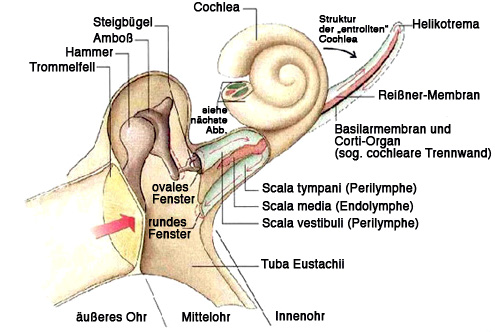
\includegraphics[width = 12cm, height = 8cm]{Ohr_Bild.jpg}
\caption{Schematische Darstellung eines Hörorgans mit abgerollter Kochlea}
\text{\footnotesize{Abruf 25.01.19 \url{http://www.eclim.de/AkuLNew/roomac_1n.html}}}
\label{fig:Ohr_Bild}
\end{figure}


Das menschliche Gehör ist in der Lage Schallereignisse mit Frequenzen von ca. 20Hz bis 16kHz - 20kHz wahrzunehmen. Dabei nimmt die Fähigkeit hohe Frequenzen zu hören um ca. 1kHz pro Lebensdekade, durch Abnutzung der Haarzellen, mit dem Alter ab \cite[S.41]{Genuit10}.  \\

\begin{figure}[H]
\centering
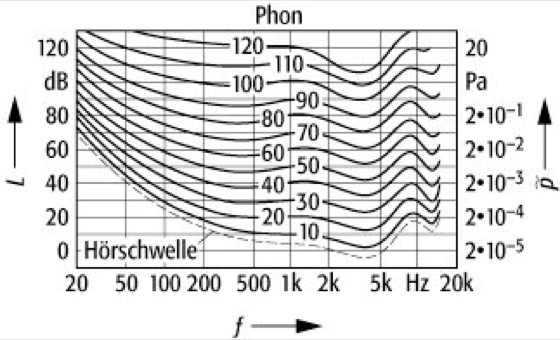
\includegraphics[width = 12cm, height = 8cm]{Kurven_gleicher_Lautheit.jpg}
\caption{Kurven gleicher Lautheit}
\text{
\footnotesize{Abruf 25.01.19 \url{https://www.spektrum.de/lexikon/physik/kurven-gleicher-lautstaerke/8648}}}
\label{fig:Kurven_gleicher_Lautheit}
\end{figure}

Der Dynamikbereich des menschlichen Gehörs wird durch die Ruhehörschwelle und die Schmerzschwelle eingegrenzt und kann hierbei frequenzabhängig zwischen 120 dB und 140 dB umfassen. Die Kurven gleicher Lautheit, siehe Abbildung \ref{fig:Kurven_gleicher_Lautheit} zeigen, dass Schallereignisse je nach Frequenz unterschiedlich laut wahrgenommen werden. Diese Frequenzabhängigkeit der empfundenen Lautheit basiert auf der Anatomie des menschlichen Ohres. Im mittleren Frequenzbereich (1 kHz bis 5 kHz) ist das menschliche Ohr am empfindlichsten. Dies ist deutlich daran zu erkennen, dass für die gleiche empfundene Lautheit bei tiefer- bzw. höherfrequenten Schallereignissen ein deutliche höherer Schalldruckpegel erreicht werden muss. Außerdem ist in diesem Bereich die Dynamik zwischen Hörschwelle (0 Phon) und Schmerzgrenze (120 Phon) am höchsten. Dies ist evolutionsbiologisch darauf zurückzuführen, dass sowohl viele Umgebungsgeräusche als auch für das Sprachverständnis wichtige Konsonanten in diesem Frequenzbereich liegen \cite[S.47]{HdA08}. 



\subsection{Verarbeitung akustischer Signale vom Zentralen Nervensystem}

Die im Zentralen Nervensystem eintreffenden Signale bilden nach der Ortstheorie des Hörens nur ein bestimmtes Frequenzband ab. Die elektrischen Signale lassen sich daher als durch Bandpassfilter verschiedener Bandbreite und Güte,  gefilterte Signale betrachten, wobei das menschliche Gehör in der Lage ist die Parameter an die zu analysierende Szene adaptiv anzupassen \cite[S.59]{Genuit10}. \\

Die Verarbeitung im Zentralen Nervensystem erfolgt nach dem Prinzip der Mustererkennung. Die Signale werden spektral analysiert werden, um Merkmale zu extrahieren und anschließend bestimmte Muster zu identifizieren und wiederzuerkennen \cite[S.51]{HdA08}. Die Betrachtung der neuronalen Prozesse zur Mustererkennung soll im Rahmen dieser Arbeit nicht weiter erläutert werden. Wichtig zu sagen ist jedoch, dass  zur Analyse von Schallereignissen  frühere Wahrnehmungen, Erfahrungen, sowie andere Sinnesreize herangezogen werden. Aus diesem Grund variiert die Wahrnehmung von Individuum zu Individuum, weshalb der Aspekt der individuellen Wahrnehmung bei der Erstellung multimedialer Inhalte stets berücksichtigt werden muss. 

\section{Räumliche Wahrnehmung}
Zur Erkennung des Ortes und der Ausdehnung werden Schallsignale nach bestimmten Merkmalen ausgewertet. Die am Trommelfell eintreffenden Schallsignale können hierbei in monoaurale und interaurale Ohrsignale kategorisiert werden. Zum Empfang monoauraler Ohrsignale ist ein Ohr ausreichend, während für den Empfang interarualer Ohrsignale beide Ohren benötigt werden. Die räumliche Wahrnehmung erfolgt sowohl durch die Analyse monoauraler als auch interauraler Ohrsignale, wobei das interaurale Hören hauptsächlich für die horizontale und das monoaurale Hören für die vertikale Wahrnehmung verantwortlich ist \cite[S.88]{HdA08}.\\

\subsection{Kopfbezogene Übertragungsfunktionen}

Das menschliche Gehör kann im technischen Sinne als Antenne betrachten werden, dessen Richtcharakteristik eine Richtungs- , Entfernungs-  und Frequenzabhängigkeit aufweist \cite[S.89]{HdA08}. Je nach Ort der Schallquelle ändert sich damit Phasengang, Gruppenlaufzeit und Frequenzgang des Schalls, der letztlich am Trommelfell ankommt. Die Veränderung der Schalls von der Quelle des Schallereignisses bis hin zur Senke, also dem Trommelfell, kann mittels sogenannter kopfbezogener Übertragungsfunktionen oder Head-Related Transfer Function (HRTF) beschrieben werden. Eine HRTF ist abhängig vom Ort der Quelle, dem Ort der Senke und dem Frequenzspektrum des Schallereignisses. Die Parameter einer HRTF $H(f,r,\phi,\delta))$ sind somit die Frequenz $f$, der Abstand zwischen Trommelfell und Schallereignis $r$ und die kopfbezogenen Richtungswinkel Azimut $\phi$ und Elevation $\delta$. Alle Parameter variieren zwischen dem linken und dem rechten Ohr, so dass immer ein binaurales Paar von HRTFs bzw. eine sogenannte interaurale Außenohr-Übertragungsfunktion $H_i$ betrachten werden muss. Diese setzt sich aus dem Verhältnis der linken HRTF $H_l$ und der rechten HRTF $H_r$ zusammen \cite[S.91]{HdA08}:

\begin{align}
H_i(f,r,\phi,\delta) = \frac{H_r(f,r,\phi,\delta))}{H_l(f,r,\phi,\delta)}
\end{align}

 Die kopfbezogenen Übertragungsfunktionen sind auf Grund der unterschiedlichen Formen von Kopf, Schultern und Außenohren des Menschen sehr individuell. In Abbildung \ref{fig:HRTF} ist dies besonders im Frequenzbereich über 7kHz zu erkennen, da die Schalldruckpegel hier sehr stark zwischen den bei Probanden gemessenen HRTFs variieren. 

\begin{figure}[H]
\centering
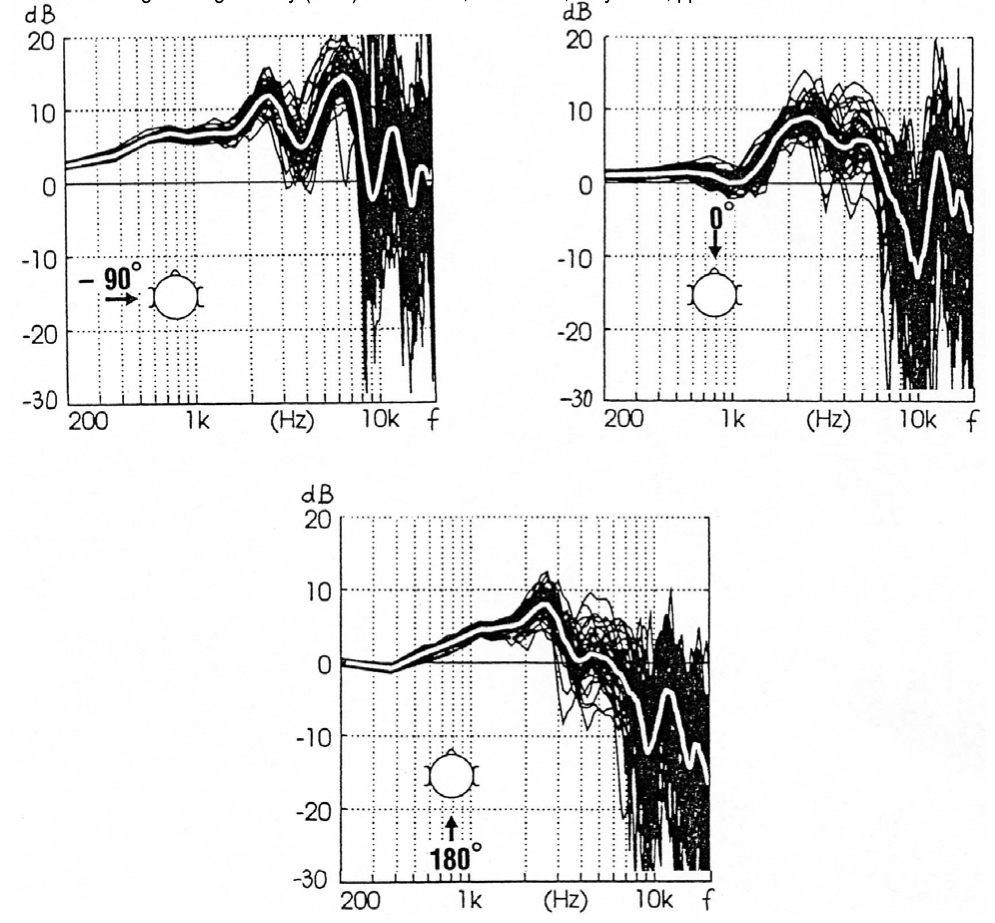
\includegraphics[width = 9cm, height = 9cm]{HRTF.jpg}
\caption{Kopfbezogene Übertragungsfunktionen eines linken Ohres}
\text{Es wurden HRTFs mehrer Personen für unterschiedlicher Richtungen aufgenommen.} 
\text{Die weißen Kurven entsprechen dem bewerteten Mittelwert.} 
\text{ \footnotesize{Abruf 25.01.19 \url{http://www.sengpielaudio.com/KopfbezogeneUebertragungsfunktionHRTF.pdf}}}

\label{fig:HRTF}
\end{figure}

\subsection{Größen des binauralen Hörens}
Wichtige Merkmale, die zur Lokalisation eines Schallereignisses analysiert werden, lassen sich aus der interauralen Außenohr-Übertragungsfunktion bestimmen. 
Nach Brauert und Braasch werden diese Größen des binauralen Hörens wie folgt berechnet \cite[S.91]{HdA08}:

\subsubsection{Interaurale Laufzeitdifferenzen}
Die interaurale Phasenlaufzeit oder auch interaurale Laufzeitdifferenz $\tau_{ph}$ berechnet sich aus dem Verhältnis der interauralen Phasendifferenz $\Delta L_i$, also der Differenz der Phase von linker zu rechter HRTF, zur Frequenz $f$ des Schallereignisses: 

\begin{align}
\tau_{ph}(f,r,\phi,\delta) = \frac{\Delta\delta_i(f,r,\phi,\delta))}{f}
\end{align}

Anhand der interauralen Laufzeitdifferenz lässt sich bestimmen an welchem Ohr der Schall bestimmter Frequenzen zuerst ankommt. Dies ist ein, für den Menschen,  wichtiges Merkmal für die Lokalisierung des Schallereignisses, da von links kommender Schall auch zu erst beim linken Ohr auftritt und umgekehrt. 

\subsubsection{Interaurale Gruppenlaufzeit}
Für die interaurale Gruppenlaufzeit wird das Verhältnis der Ableitung der interauralen Phasendifferenz zur Frequenz $f$ des Schallereignisses berechnet: 
\begin{align}
\tau_{gr}(f,r,\phi,\delta) = \frac{d\Delta\delta_i(f,r,\phi,\delta))}{f}
\end{align}

Die interaurale Gruppenlaufzeit gibt im Gegensatz zur interauralen Laufzeitdifferenz an, bei welchem Ohr die Einhüllende des Schallereignisses zu erst ankommt und wie stark verzögert sie das zweite Ohr erreicht. 


\subsubsection{Interaurale Pegeldifferenzen}

Die interaurale Pegeldifferenz $\Delta L_i$ wird als logarithmisches Maß zur Beschreibung der Intensitätsunterschiede des Schalls verwendet, der an beiden Ohren ankommt: 

\begin{align}
\Delta L_i = 20* \lg(H_i(f,r,\phi,\delta)) 
\end{align}


\subsection{Funktionsweise der Schallquellenortung}

Das Außenohr, der Kopf und die Schultern wirken alle als richtungs-, entfernungs- und , frequenzabhängige Filter für den am Trommelfell ankommenden Schall. Ist dem Hörenden ein Schallereignis bekannt, so ist er in der Lage die Filtereigenschaften zu bestimmen und so Rückschlüsse auf die Position des Schallereignisses zu ziehen.

\begin{figure}[H]
\centering
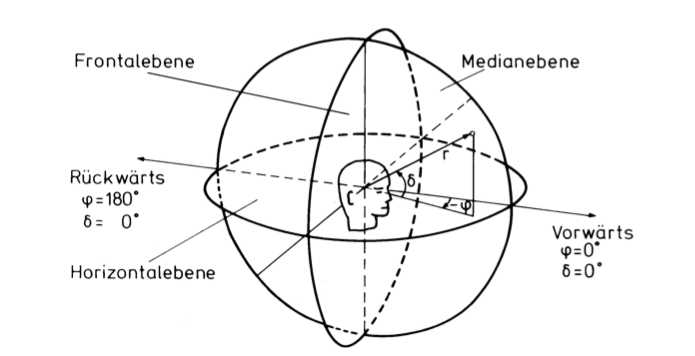
\includegraphics[width = 12cm, height = 6cm]{kopfbezogenes_Koordinatensystem.png}
\caption{Kopfbezogenes Koordinatensystem}
\text{Nach Blauert und Braasch \cite[S.88]{HdA08}}
\label{fig:Kopfbezogenes_Koordinatensystem}
\end{figure}

\subsubsection{Richtungswahrnehmung}

Schallquellen innerhalb der Frontal- und Horizontalebene können anhand von interauralen Laufzeitdifferenzen, interauralen Pegeldifferenzen sowie interauralen Gruppenlaufzeitunterschieden lokalisiert werden. Der Kopf des Menschen weist eine Filtercharakteristik für hohe Frequenzen auf. Wellenlängen, die kleiner als der Kopf selbst sind, werden durch diesen gedämpft. Die Ortung hoher Frequenzen erfolgt daher weitestgehend durch die Analyse der Gruppenlaufzeit und der Pegeldifferenzen, da die Einhüllende des Schalls durch den Kopf weniger stark beeinflusst wird. Die Lokalisierung niederfrequenten Schalls erfolgt dahingehend durch die Verarbeitung der Laufzeit- und Pegeldifferenzen \cite[S.45]{Genuit10}. \\ 

Die monoauralen Außenohrübertragungsfunktionen weisen auf Grund der Struktur des Außenohres eine signifikante Abhängigkeit zum Einfallswinkel des Schalls auf. Dadurch ist es dem Menschen erlaubt schon geringe Positionsänderungen der Schallquelle zur Medianebene  wahrzunehmen \cite[S.46]{Genuit10}. \\ 

Die horizontale Wahrnehmung ist empfindlicher als die vertikale Wahrnehmung. In der Horizontalebene werden Richtungsänderungen ab ca. 4 grad und in der Frontalebene erst ab ca. 10 grad merklich wahrgenommen \cite[S.95]{HdA08}.  \\

Die Lokalisation von Schallquellen in der Medianebene  basiert auf der Verarbeitung monoauraler Merkmale, da durch die Position der Schallquelle der Direktschall für beide Ohren annähernd identisch ist. Auch hier gilt, dass die Filterwirkung von Außenohr und Körper, speziell die Schultern, den Schall so beeinflussen, dass Änderungen des Klangs zur Richtungslokalisation interpretiert werden können \cite[S.46]{Genuit10}. \\

Wellenlängen, die größer als die Ohrmuschel selbst sind, werden durch das Ohr kaum beeinflusst. Daraus resultiert, dass die Filterwirkung des Außenohres sich auf Frequenzen oberhalb von ca. 3,5 kHz begrenzt. Die Richtungslokalisation von Schallquellen in der Horizontal- und Frontalebene erfolgt daher besonders gut bei höherfrequenten Schallereignissen \cite[S.47]{Genuit10}.

Ein wichtiger Aspekt der Richtungslokalisation ist die Fähigkeit des Menschen seinen Kopf zu bewegen. Die dadurch entstehenden Änderungen der interauralen Laufzeit- und Intensitätsdifferenzen lassen sich zeitlich analysieren, so dass die Richtung des Schalls leichter erkannt werden kann \cite[S.88]{HdA08}.

\subsubsection{Entfernungswahrnehmung}

Wie bei der Richtungslokalisation gelingt auch das Entfernungshören aufgrund der Verarbeitung von mono- sowie interauralen Merkmalen.

Ist die Schallquelle dem Hörenden sehr nahe (weniger als 25cm entfernt) so bewirkt die Abschirmung durch den Kopf, dass der Schall bei einem Ohr stark gedämpft ankommt. Die interaurale Pegeldifferenz ist daher für die Entfernungseinschätzung naher Schallquellen von herausragender Bedeutung \cite[S.98]{HdA08}.\\

Des Weiteren wird auch der allgemeine Signalpegel zur Entfernungseinschätzung genutzt. Ist ein Signal leiser so ist davon auszugehen, dass die Quelle weiter entfernt ist \cite[S.98]{HdA08}.\\

Ist die Schallquelle zwischen 25cm und 15m vom Hörer entfernt spricht man vom mittleren Entfernungsbereich. Bei Kugelstrahlern 0. Ordnung, im freien Schallfeld, erzielt eine Abstandsverdopplung der Quelle zum Hörer, in diesem Bereich, eine Steigerung des Signalpegels um 6dB \cite[S.98]{HdA08}. In einem Raum gilt, dass die Menge an Direktschall, der am Trommelfell ankommt, mit der Entfernung abnimmt. Aus diesem Grund ist das Verhältnis von Direktschall zu diffusem Schall ein weiteres informatives Merkmal zu Einschätzung von Entfernungen \cite[S.57]{Heidermanns1979}.
\\

Die Entfernung zu Hörereignissen, die weiter als 15m entfernt sind, kann ohne Hintergrundwissen, wie z.B visuelle Eindrücke, nicht geschätzt werden. Da Schall über weite Entfernung jedoch frequenzabhängig gedämpft wird, lässt sich anhand des dumpfen Klangs beurteilen, ob die Schallquelle weit entfernt sein muss \cite[S.99]{HdA08}. 

\subsection{Im-Kopf-Lokalisation}

Sind die Schallquellen sehr nah, z.B bei Kopfhörern, kann es zur sogenannten Im-Kopf-Lokalisation kommen. Das Schallereignis wird hierbei im Kopf statt vor den Ohren lokalisiert. \\ 

Die Filterwirkung des Außenohrs und die Beschallung der Schädelknochen, die ebenfalls vom Gehör analysiert werden kann, fallen bei der zu nahen Beschallung weg. Da dies natürlicherweise nicht vorkommt ist das Gehör nicht daran gewöhnt Schall zu analysieren der nicht durch das Außenohr entzerrt worden ist. Der Im-Kopf-Lokalisation kann daher durch eine vorherige Entzerrung der Ohrsignale entgegengewirkt werden, so dass auch über Kopfhörer entfernte Schallquellen simuliert werden können \cite[S.47]{Blauert80}.

\subsection{Schallquellenortung bei mehreren Schallquellen}

Bei der Hörereignisbildung mit mehreren Schallquellen treten verschiedenste Effekte auf. Die wichtigsten Effekte sollen im Sinne dieser Arbeit kurz erläutert werden, um ihren Einfluss beim Hörversuch einschätzen zu können. 

\subsubsection{Summenlokalisation - Phantomschallquellen}

Bei zwei Schallquellen, die das selbe Signal wiedergeben und gleich weit vom Hörenden entfernt sind,siehe Abbildung \ref{fig:Stereoaufstellung_Phantomschallquelle}, wird das Hörereignis zentral zwischen den beiden Schallquellen gebildet. Diese Summenlokalisation der Ohrsignale führt zur Bildung einer imagniären Schallquelle, welche zentral zwischen den realen Schallquellen lokalisiert wird. Diese imaginären Schallquellen werden als Phantomschallquellen bezeichnet  \cite[S.101]{HdA08}.
Die Richtungslokalisation ist jedoch bei Phantomschallquellen in der Regel fehleranfälliger als bei realen Schallquellen. Dies gilt besonders bei der seitlichen Bildung von Phantomschallquellen mit Surround-Sound  \cite[S.103]{HdA08}. 

\begin{figure}[H]
\centering
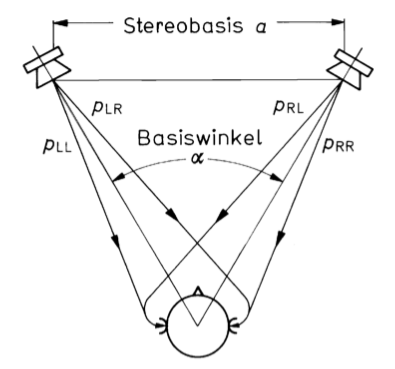
\includegraphics[width = 8cm, height = 6cm]{Stereoaufstellung_Phantomschallquelle.png}
\caption{Stereolautsprecher-Anordnung} 
\text{\cite[S.101]{HdA08}}
\label{fig:Stereoaufstellung_Phantomschallquelle}
\end{figure}

Bei der Summenlokalisation werden Laufzeit- und Pegeldifferenzen zwischen den beiden Lautsprechersignalen analysiert, um die Phantomschallquelle zu orten. Ist ein Signal stärker als das andere  wird die Phantomschallquelle eher in Richtung der lauteren, realen Quelle lokalisiert. Gleichzeitig wird die Phantomschallquelle eher in Richtung der realen Schallquelle lokalisiert, dessen Schall früher beim Hörenden ankommt. Bei größeren Verzögerungen kommt es zum sogenannten Präzedenzeffekt. \\ 

Anhand der Abbildung \ref{fig:Summenlokalisationskurven} lässt sich erkennen, dass die Richtungszuordnung in keinem linearen Zusammenhang zu wahrgenommenen Laufzeit- und Pegeldifferenzen steht. Des Weiteren ist zu erwähnen, dass sich die Auswirkung der Laufzeit- und Pegeldifferenzen gegenseitig beeinflussen und aufheben können \cite[S.103]{HdA08}. 
 
\begin{figure}[H]
\centering
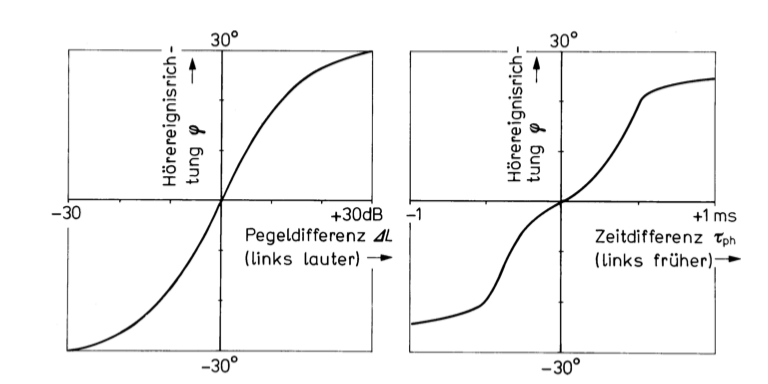
\includegraphics[width = 14cm, height = 8cm]{Summenlokalisationskurven.png}
\caption{Summenlokalisationskurven für Pegel- und Laufzeitdifferenzen der beiden Lautsprechersignale} 
\text{\cite[S.101]{HdA08}}
\label{fig:Summenlokalisationskurven}
\end{figure}

\subsubsection{Präzedenzeffekt}

Bei der Wiedergabe eines Signals über mehrere Lautsprecher wird ,nach dem Gesetz der ersten Wellenfront, die Hörereignisausrichtung fast ausschließlich anhand des ersten eintreffenden Schalls vorgenommen. Die Signale, die mit mehr als einer Millisekunde Verzögerung eintreffen werden dann als indirekter Schall gewertet, so dass dieser nur zur Lautstärke beiträgt und nicht zur Richtungslokalisation. Dies ermöglicht es auch in geschlossen Räumen ein Hörereignis trotz mehrfach reflektierten Schalls zu orten \cite[S.103]{HdA08}. \\

Treffen Signale mit einer Verzögerung von mehr als 50 ms auf wird der Schall nicht als indirekter Schall sondern als Echo erkannt. Dies bewirkt, dass der Schall nicht in die Summenlokalisation für die Position der ersten Quelle  mit einbezogen wird, sondern stattdessen als einzelnes Hörereignis mit eigener Quelle erkannt wird. Besitzt ein Signal einen deutlichen höheren Pegel als die vorherigen Signale kann es auch bei einer geringeren Verzögerung als 50ms schon als Echo gedeutet werden \cite[S.49]{Genuit10}. 
 

\subsubsection{Binaurale Störgeräuschunterdrückung/ Cocktailparty-Effekt}

Der Mensch ist in der Lage den Schall in seiner Umgebung zu analysieren und zwischen Nutzschall und Störgeräuschen zu unterscheiden. Durch die Lokalisation der Nutzschallquelle, z.B. einer sprechenden Person, kann bewusst die Wahrnehmung anderer Störschallquellen unterdrückt werden (Cocktailparty-Effekt). Die Analyse interauraler Laufzeit- und Pegeldifferenzen ermöglicht eine Dämpfung des Störschalls zwischen 9 und 15 dB. Die Effektivität der Störschallunterdrückung ist abhängig von der Richtung des einfallenden Schalls \cite[S.48]{Genuit10}. 

\section{Zusammenspiel mehrerer Sinnesreize }
Für die Deutung der akustischen Signale vom Zentralen Nervensystem werden, neben den akustischen, weitere Sinnesreize herangezogen. Im Rahmen der Versuches dieser Arbeit werden Probanden sowohl optischen als auch akustischen Sinnesreizen unterzogen. Wie sich die Wahrnehmungen dieser Reize gegenseitig beeinflussen und welche Effekte hierbei auftreten können soll im Folgenden erläutert werden.

\subsection{Einfluss des Visuellen auf die auditive Wahrnehmung}
Die Einordnung des Schallereignisses mittels einer Mustererkennung im Gehirn des Menschen basiert darauf, dass Merkmale aus den aktuell eintreffenden Reizen gebildet werden. Solch ein Merkmal könnte beispielsweise eine bestimmte spektrale Zusammensetzung sein. Die Menge aller Merkmale wird daraufhin mit Merkmalen vergangener Ereignisse verglichen. Korreliert hierbei eine Merkmalsmenge mit der eines vergangen Ereignisses, so kann das Zentrale Nervensystem das Schallereignis kategorisieren und einordnen \cite[S.51]{HdA08}. Neben akustischen Merkmalen werden auch aus optischen Reizen Merkmale gebildet \cite[S.88]{HdA08}. Die Wahrnehmungsfähigkeit des Menschen steigert sich durch den Einsatz mehrerer Sinnesreize  enorm, da es  dem Zentralen Nervensystem so ermöglicht eine größere Menge an Merkmalen zu bilden, irrelevante Merkmale leichter auszusortieren und auf einen größeren Erfahrungsschatz  zurückzugreifen. \\ 

\subsection{Hörausrichtung an Blickrichtung}

Neben diesem psychologischen Aspekt, muss der physiologische Aspekt der Anpassung der Richtcharakteristik des Gehörs an die Blickrichtung mit herangezogen werden. Der Mensch ist nachweislich in der Lage sowohl die Ausrichtung des Trommelfells als auch die Stellung der Haarzellen in der Kochlea an die  Blickrichtung anzupassen, um Hörereignisse, auf die er sich fokussiert, besser hören zu können. Dabei geschieht die Ausrichtung der Gehörkomponenten sogar vor dem Wechsel des Blickpunkts\cite{Strick17}. Eine Visualisierung der akustischen Szene kann also dafür sorgen, dass gezielt bestimmte Inhalte besser gehört werden können, in dem diese visuell Aufmerksamkeit auf sich ziehen.  

\subsection{Bauchredner-Effekt}

Treffen akustischer und optischer Reiz synchron, also mit einer Verzögerung von maximal ca. 50- 100ms,  auf können sich die individuellen Wahrnehmungen gegenseitig beeinflussen. Für die Deutung der auditiven Merkmale ist der optische Reiz hierbei von größerer Bedeutung als es umgekehrt der Fall ist. Bauchredner versuchen auf diese Weise dem Publikum die Lokalisation der wahren Schallquelle zu erschweren. Der sich bewegende Mund der Puppe stellt stellt einen optischen Reiz dar, der mit dem Hörereignis des sprechenden Redners übereinstimmt. In Folge dessen wird die wahrgenommene Schallquelle auf den Mund der Puppe projiziert \cite[S.163]{Genuit10}.

Obwohl visueller und akustischer Reiz nicht zusammen passen wird die Gesamtsituation vom Konsumenten als plausibel wahrgenommen. Dies bedeutet, dass ein perfektes Panning der auditiven Signale für eine plausible Wiedergabe nicht immer von Nöten ist. Andererseits ist aber auch zu beachten, welchen visuellen Reizen der Konsument im Moment der auditiven Wiedergabe untersetzt ist. Schaut der Betrachter im Moment der auditiven Wiedergabe auf eine potentielle, alternative Schallquelle  kann es zu ungewollter Fehllokalisation der Hörereignisse stattfinden kann.



\section{Wohlbefinden bei akustischen Szenen}
Damit virtuell erstellte Medien bei den Kunden Anklang finden müssen diese sich beim Konsum vor allen Dingen wohlfühlen. Gerade im Bereich AR und VR geht es oft darum, dass akustische und visuelle Szenen so realistisch wie möglich dargestellt werden, dabei ist bereits bewiesen, dass zu realistische, visuelle Szenen eher Unbehagen als Begeisterung beim Konsumenten bewirken. Im Rahmen dieser Arbeit soll dahingehend auch geprüft werden inwiefern bei akustischen Szenen solch ein Unbehagen ausgelöst werden kann und wie sich die Versuchsprobanden bei der Darbietung der audiovisuellen Szenen fühlen. 

 \subsection{Immersion}
 
 Virtual Reality wird häufig mit dem Wort Immersion in Verbindung gebracht. Als Immersion bezeichnet man die Einhüllung in Medien. Im Folgenden soll kurz der Zustand der Immersion erläutert und im Anschluss der Zusammenhang zu den Themen dieser Bachelorarbeit geschlossen werden. \\

Nach Grau äußere sich die Immersion in dem Moment in dem der Betrachter die kritische Distanz zum Medium verliere und die emotionale Involvierung ansteige \cite[S.13]{Grau03}. Der Konsument wird im Zustand der Immersion also Teil der medialen Szene und ist in der Lage seine reale Umgebung komplett auszublenden. Auch wenn dies schon bei älteren Medien wie Fernsehen oder Theater der Fall gewesen ist, so ist dieser Zustand mit dem Einsatz von VR und AR noch intensiver zu verwirklichen.  \\

\begin{figure}[H]
\centering
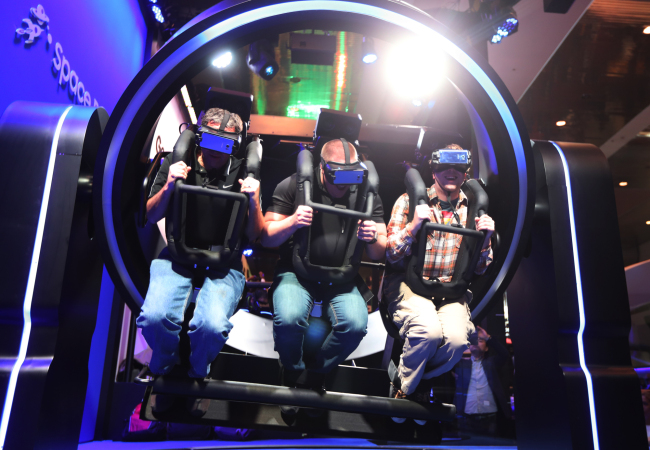
\includegraphics[width = 11cm, height = 7cm]{VR_Immersion.jpg}
\caption{Immersives Erlebnis durch Achterbahnsimulation mit der Samsung Gear}
\text{\footnotesize{Abruf 29.01.19: \url{http://forums.cgsociety.org/t/samsung-gear-vr-fully-immersive-4d-experience/1810570}}}
\label{fig:VR_Immersion}
\end{figure}
\newpage

Virtual Reality biete hierbei Techniken, die traditionelle Medien polysensorisch erlebbar machen würden, behauptet Grau \cite[S.15]{Grau03}  In diesem Zusammenhang wurde besonders der Aspekt der freien Kopfbewegung genannt, der es ermögliche die Szene aus unendlich vielen Perspektiven zu beobachten. Auch der Einsatz von räumlichem Audio sowie die Interaktion mit der virtuellen Welt erlaube ein noch stärkeres Gefühl der Immersion \cite[S.16]{Grau03}. \\
 
 Damit die synthetisch erschaffene Welt eine Immersion zulasse, müsse diese nicht die Umgebung komplett umfassen, beziehungsweise realistisch sein, sondern stattdessen plausibel\cite[S.17]{Grau03}. Die Stärke der Immersion hänge dabei zum einen von der Glaubwürdigkeit, aber auch von der Genießbarkeit der Illusion ab\cite[S.17]{Grau03}. \\
 
 Die Immersion ist im Zusammenhang mit dem Einsatz von räumlichem Audio ein erstrebenswerter Zustand für den Konsumenten. Dieser soll den Eindruck vermittelt bekommen, dass die ihm dargebotene virtuelle Szene Wirklichkeit sein könnte, so dass dieser die Realität ausblendet.
 
In den Versuchen dieser Arbeit soll eine virtuelle Welt in die reale Welt integriert werden. Hierbei werden visuelle und auditive Inhalte im Raum platziert und über eine Microsoft Mixed Reality Brille wiedergegeben. In diesem Zusammenhang würde eine Immersion bedeuten, dass der Konsument die dargebotenen, virtuellen Inhalte  als Teil seiner realen Umgebung wahrnimmt. 
 
 Nicht nachvollziehbare Reize können eine Immersion beim Konsumenten verhindern\cite[S.17]{Grau03}. Im Zusammenhang mit den Versuchen bedeutet dies, dass sowohl auditive und visuelle Inhalte, als auch reale und virtuelle Welt zueinander kompatibel sein müssen und plausible Sinneseindrücke bewirken müssen. 
 
 Um das Immersionsempfinden der Probanden während des Hörversuchs zu überprüfen werden, die Probanden gebeten die Darbietung nach den Kriterien der Plausibilität, dem Realismus der auditiven Inhalte und ihrem eigenen Wohlbefinden für jede Szene zu bewerten.
 
\subsection{Das Uncanny Valley und der Bezug zur Immersion bei VR und AR}

Das Uncanny Valley ist ein Begriff der Robotik, der zum ersten mal vom japanischen Robotiker Masahiro Mori 1970 verwendet worden ist. Dieser beschreibe die verminderte Vertrautheit des Menschen gegenüber synthetisch erstellten Figuren, wenn diese eine bestimmte Intensität des Anthropomorphismus (Menschenähnlichkeit) aufweisen \cite{Mori70}.

\begin{figure}[H]
\centering
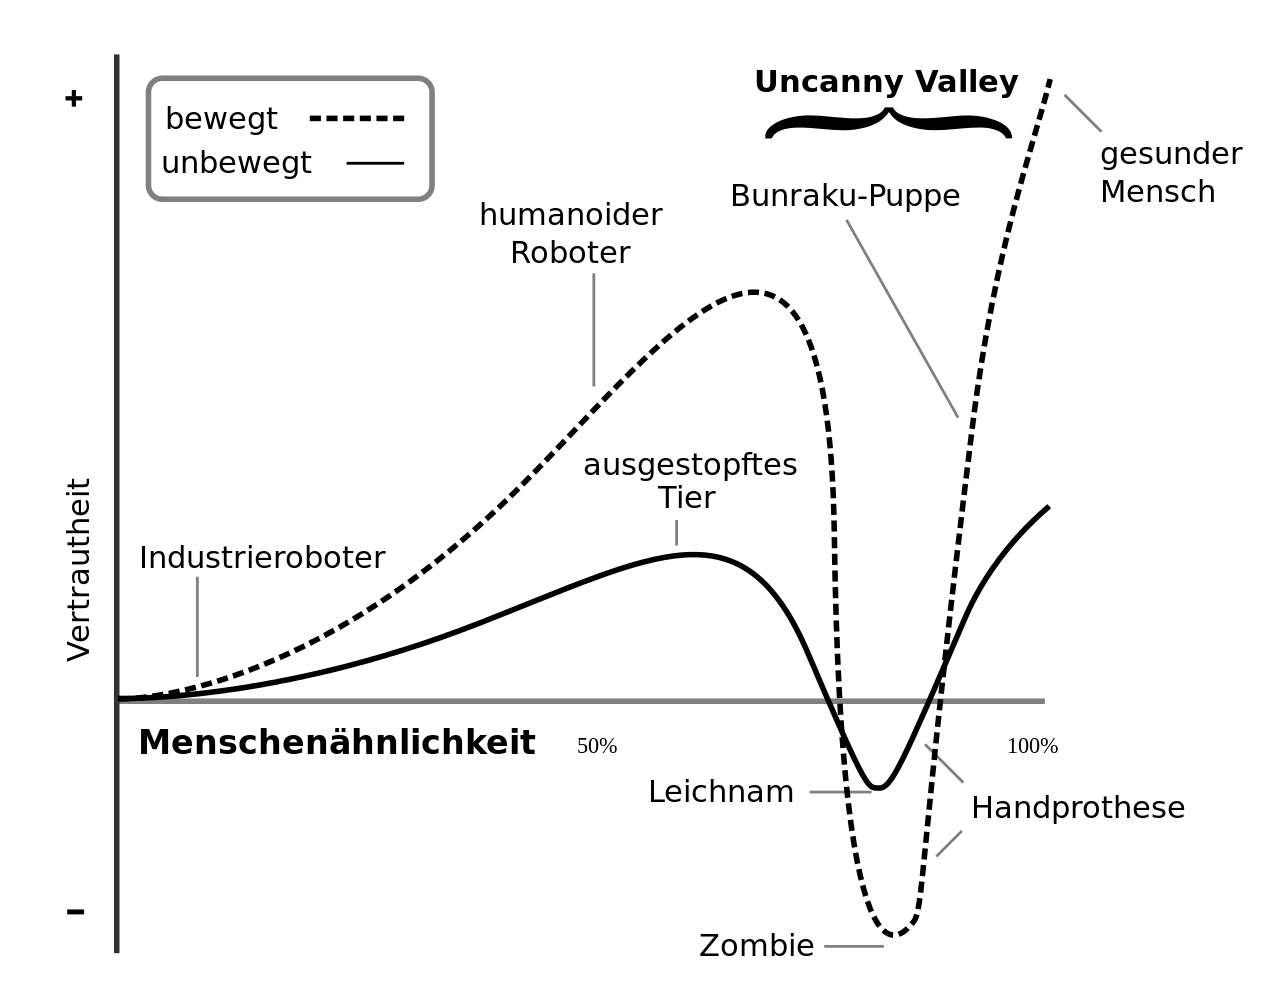
\includegraphics[width = 10cm, height = 7cm]{Mori_Uncanny_Valley_de.png}
\caption{Darstellung des Uncanny Valley mit Einordnung verschiedener Figuren} 
\text{Abbildung von Mori 1970 $ - $Übersetzung durch Tobias K.}
\text{\footnotesize{Abruf 23.01.19: \url{https://de.wikipedia.org/wiki/Datei:Mori_Uncanny_Valley_de.svg}}}
\label{fig:Mori_Uncynn_Valley_de}
\end{figure}

Wie in Abbildung \ref{fig:Mori_Uncynn_Valley_de} zu erkennen ist steigt die Akzeptanz des Betrachters gegenüber der visuellen Erscheinung zunächst mit steigernder Menschenähnlichkeit an, bis sie abrupt ab einem bestimmten Realitätsgehalt in eine starke Befremdlichkeit übergeht. Anschließend steigt diese Vertrautheit jedoch wieder mit der Menschenähnlichkeit an. Bei bewegten Figuren ist dieser Effekt noch stärker zu beobachten. Der Bereich des starken Abfalls und Wiederanstieg der Vertrautheitskurve wird als Uncanny Valley bezeichnet \cite{Mori70}.\\

Die Akzeptanzlücke gegenüber realistischen,künstlich entstandenen, visuellen Reizen, die beim Menschen von Mori beobachtet worden ist, lässt vermuten, dass die Befremdlichkeit gegenüber synthetisierten Szenen, sowohl visuell als auch auditiv, mit dem Realitätsgehalt der Medien zunehmen könnte. \\ 

Große Firmen der Unterhaltungsindustrie wie Sony und Oculus rieten Entwicklern daher schon auf der Game Developers Conference in Köln 2014, dass diese ihre VR- und AR-Anwendungen nicht zu realistisch gestalten dürfen, da der Effekt des Uncanny Valley drohe. Des Weiteren dürfe man die Blickrichtung des Benutzers nicht einschränken und müsse Phobien wie Klaustrophobie oder Höhenangst beachten. VR-Erlebnisse sollen demnach "eher als Analogie zu einem Ritt durch einen Vergnügungspark begriffen werden als zu einem Kinofilm" \cite{Gieselmann}. \\
 
 Im Zuge dieser Arbeit werden Audioszenen betrachtet die extremen Realismus implizieren könnten. Es ist nicht auszuschließen, dass auch mit steigendem Realitätsgehalt auditiver Szenen bzw. räumlichem Audio eine Art "Uncanny Valley"-Effekt beim Hörenden entsteht. In Anbetracht dessen solltet es umso wichtiger sein, während des Hörversuchs, das Wohlempfinden der Probanden zu beobachten.  Die Erforschung, ob es wirklich ein Art "Uncanny Valley" für räumliches Audio gibt, ist ein wichtiges Thema für die Weiterentwicklung von AR und VR. Es übersteigt jedoch den Rahmen dieser Bachelorarbeit und wird deshalb nur angerissen.
 
 \chapter{Technische Grundlagen}
Der im Rahmen dieser Arbeit durchzuführende Hörversuch beinhaltet einen typischen Anwendungsfall für eine AR-Anwendung. Eine virtuelle Welt wird mit Hilfe einer Microsoft Mixed Reality Brille auf einen realen Tisch projiziert.  Es folgt die binaurale Wiedergabe von Schallereignissen über virtuelle Punktschallquellen im Raum, die es von den Probanden zu lokalisieren gilt. Ziel hierbei soll sein, die Lokalisationsfähigkeit und das Darbietungsempfinden der Probanden bei räumlichem Audio für einen realistischen Anwendungsfall zu analysieren. Dafür ist eine AR-Applikation entwickelt worden, mit der die Durchführung und Dokumentation des Hörversuchs automatisiert wird.

Die zur Erstellung der Applikation notwendigen technischen Grundlagen sowie die verwendete Hard- und Software sollen im Folgenden veranschaulicht werden. 

 \section{Augmented Reality}
Die Erweiterte Realität , engl. Augmented Reality (AR), ist eine Variation der Virtuellen Realität, engl. Virtual Reality (VR). Während bei VR-Anwendungen versucht wird den Benutzer komplett in einer synthetisierten Welt eintauchen zu lassen, geht es bei AR darum die physische Welt des Benutzers virtuell zu ergänzen \cite{Azura97}. \\

\begin{figure}[H]
\centering
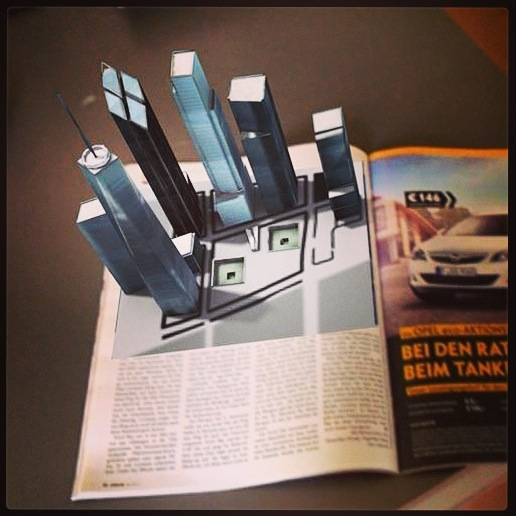
\includegraphics[width = 8cm, height = 6cm]{AR_Beispielbild.jpg}
\caption{Zeitschrift dessen Inhalt durch virtuelle Objekte ergänzt wird}
\text{\footnotesize{Abruf 22.01.19:}}
\text{\footnotesize{\url{https://www.dpc-consulting.org/augmented-reality-aktuelle-beispiele-fur-verlage-und-medienhauser/}}}
\label{fig:AR_Beispielbild}
\end{figure}

Im Hörversuch dieser Bachelorarbeit sollen die Probanen in eine AR-Umgebung eintauchen, bei der der reale Raum mit einer audiovisuellen, virtuellen Welt überlagert wird. 

\subsection{Microsoft Mixed Reality}
Microsoft verwendet im Zusammenhang mit AR und VR häufig den Begriff Microsoft Mixed Reality und bezeichnet auch ihre Head Mounted Displays als Microsoft Mixed-Reality Brillen. Nach der Dokumentation von Microsoft  beinhaltet Microsoft Mixed Reality neben der virtuellen Erweiterung der Realität auch die Interaktion zwischen Mensch, Maschine und Umgebung \cite{MicrosoftMR}. 


\begin{figure}[H]
\centering
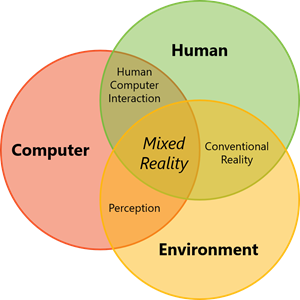
\includegraphics[width = 8cm, height = 8cm]{Mixed_Reality.png}
\caption{Zusammensetzung von Mixed Reality}
\text{\footnotesize{Abruf 07.02.19:}}
\text{\footnotesize{\url{https://docs.microsoft.com/en-us/windows/mixed-reality/mixed-reality}}}
\label{fig:Mixed_Reality}
\end{figure}
 
Microsoft bietet mit Microsoft Mixed Reality Gestensteuerung, Spracherkennung, Kopfverfolgung (Head-Tracking), Kopfbezogene Übertragungsfunktionen(HRTF) und weitere Funktionen an. Dabei können sogar auditive und visuelle Inhalte an die physischen Gegebenheiten des Raums angepasst werden. Entwicklern werden diese Funktionen umsonst mit dem MixedRealityToolkit zur Verfügung gestellt, dessen Funktionalitäten wiederum in Unity3D importiert werden können. Auf diese Art und Weise können AR- und VR-Anwendungen erstellt werden, die sowohl räumliches Audio als auch eine an Mixed Reality Brillen angepasste Steuerung ermöglichen. Die wichtigsten verwendeten Funktionen des Toolkits und von Unity3D werden im Verlauf der Arbeit noch individuell betrachtet.


\section{Microsoft HoloLens}
Als Wiedergabegerät während des Hörversuchs wird eine Microsoft HoloLens verwendet, siehe Abbildung \ref{fig:microsoft_hololens}. Bei dieser handelt es sich um eine Microsoft Mixed Reality Brille, die mit einem Head-Mounted-Display, Kopfhörern, Head-Tracking-Funktion sowie einem Natural-User-Interface ausgestattet ist.

 \begin{figure}[H]
\centering
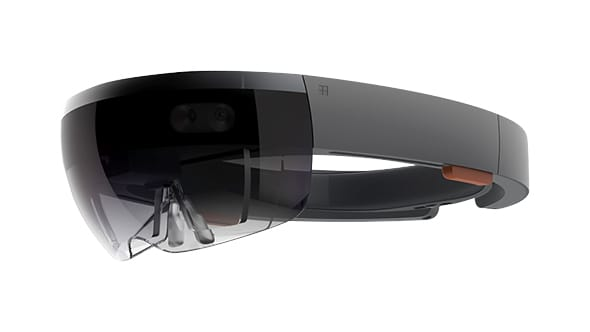
\includegraphics[width = 8cm, height = 6cm]{microsoft_hololens.jpg}
\caption{Mixed-Reality Brille - Microsoft HoloLens}
\text{\footnotesize{Abruf 23.01.19:}}
\text{\footnotesize{\url{https://www.macerkopf.de/2016/10/12/microsoft-hololens-kommt-im-november-nach-deutschland}}}


\label{fig:microsoft_hololens}
\end{figure}

\subsection{Head-Mounted-Displays}
Für die Umsetzung von AR- und VR-Anwendungen werden sogenannte Head-Mounted-Displays verwendet, welche dem Nutzer ermöglichen sollen möglichst realitätsnah visuelle Reize wahrzunehmen. Die Bildschirme in der Brille projizieren virtuelle Inhalte direkt in das Auge des Benutzers, so dass dieser denken soll Teil der virtuellen Umgebung zu sein. Bei AR-Brillen bzw. der Mixed Reality Brille Microsoft HoloLens wird hierbei ein transparenter Bildschirm verwendet, der es ermöglicht neben der virtuellen auch die reale Welt zu sehen.\\


\subsection{Kopfhörer der HoloLens}
Die Kopfhörer befinden sich an der Unterseite des Haltemechanismus der Brille. Sie sind über den Ohren positioniert, bedecken diese aber nicht. Auf diese Weise lassen sie die Umgebungsgeräusche ungedämpft durch. Dies ist vor allem dann wichtig wenn es um die Lokalisationsfähigkeit von Hörereignissen in der Umgebung des Nutzers geht. Wie bereits im Unterkapitel "räumliche Wahrnehmung" beschrieben wird, bewirkt die individuelle Außenohrform eine spektralen Verzerrung des Schall und ist für die spektrale Analyse zur Lokalisation von Hörereignissen von herausragender Bedeutung. Ohrenumschließende Kopfhörer sollten daher theoretisch für eine AR-Anwendung mit auditiver Überlagerung nur bedingt geeignet sein, da diese frequenzabhängig dämpfen und die Form der Ohrmuschel durch Druck verändern können.

\subsection{Head-Tracking-Funktion}
Die HoloLens bietet eine Head-Tracking-Funktion, die es erlaubt die Hörsignale an die Ausrichtung des Kopfes anzupassen. Dies ist wichtig, da die Rotation des Kopfes neben der offensichtlichen Veränderung des Blickfeldes auch eine Veränderung des an den Ohren ankommenden Schalls bewirkt. Die Analyse der damit einhergehenden Änderungen der interauralen Laufzeit- und Pegeldifferenzen tragen maßgeblich dazu bei Hörereignisse zu lokalisieren. Die für den Hörversuch entwickelte HoloLens-App erlaubt die freie Bewegung des Probanden im Raum und die freie Bewegung des Kopfes. Auf diese Art und Weise sollte die Lokalisation von virtuellen Schallquellen im Vergleich zu statischen Wiedergabesystemen ohne Head-Tracking, stark vereinfacht werden und den Realismus der audiovisuellen Szenen verstärken.  
  
\section{Binaurale Wiedergabe}
 Das Problem der binauralen Wiedergabe räumlicher auditiver Szenen über Kopfhörer ist, dass die Beeinflussung des Schalls durch die Umgebung auf dem Weg zum Trommelfell nicht gegeben ist. Es werden also weder Schallreflexionen, noch die Filterwirkung des Körpers und der Außenohren auf den Schall wahrgenommen. Die Lokalisation von Schallereignissen über Kopfhörer ist dementsprechend nur dann möglich wenn die binauralen Signale angepasst werden. 
 
 \subsection{Kopfbezogene Übertragungsfunktionen - MS HRTF Spatializer}
 
 Die bereits im Kapitel "Menschliche Wahrnehmung" behandelten kopfbezogenen Übertragungsfunktionen beschreiben das System zwischen der Quelle eines Schallereignissen und der Senke, also dem Trommelfell. Die Faltung des Audio-Signals mit der zugehörigen HRTF verändert den eintreffenden Schall so, als ob er durch den Körper und die Außenohren gefiltert worden wäre. \\
 
 Technisch gesehen wird räumliches Audio dadurch realisiert, dass je nach Position der virtuellen Schallquelle zum Kopf ein HRTF-Paar aus einer Datenbank ausgewählt und mit dem wiederzugebenden Audio-Signal digital gefaltet wird. Auf diese Art und Weise werden interaurale Laufzeit- und Pegeldifferenzen dem trockenen Signal hinzugerechnet, so  dass auch über  binaurale Wiedergabe eine Schallquellenlokalisation stattfinden kann. Für die Applikation wurde der von Microsoft entwickelte MS HRTF Spatializer verwendet,der ebenfalls nach diesem Prinzip arbeitet \cite{MSHRTF}.
 
 Damit die Lokalisationsfähigkeit bei binauraler Wiedergabe vollständig gegeben ist muss für jeden Menschen ein individueller Datensatz an HRTFs verwendet werden. Dies spiegelt sich besonders im Bereich der Lokalisation hochfrequnter Schallereignisse wieder, da hier, durch die individuelle Außenohrform, die HRTFs am stärksten variieren.
 Ein weiterer Ansatz der personalisierten HRTF-Datensätze besteht darin über neuronale Netze und Methoden des Machine Learnings die HRTF-Datensätze automatisch an den Benutzer anzupassen \cite{MSHRTF}. 
 
 Da die Aufnahme individueller HRTF-Datensätze für jeden Probanden der Versuche den Rahmen dieser Bacherlorarbeit übersteigen würde, wird für die Durchführung der Versuche ein einzelnder HRTF-Datensatz verwendet. Bei der Auswertung der Versuchsergebnisse muss daher berücksichtigt werden, dass der genutzte HRTF-Datensatz unterschiedlich stark mit den wirklichen HRTF-Datensätzen der Probanden korreliert. Dies gilt besonders bei der Betrachtung hochfrequenter Schallereignisse über 7kHz. 
 
 \subsection{Auralisation} 

Auralisation beschreibt Verfahren die es ermöglichen Schallsignale so zu verändern, dass es so klingt als wären diese in einem bestimmten Raum aufgenommen worden. Die Faltung eines Audio-Signals mit der monoaural-aufgenommenen Raumimpulsantwort ermöglicht es den individuellen Klang des gewünschten Raumes  in das  Schallsignal zu übertragen und so ein plausible Schallereignisse zu erzeugen  \cite[S.521]{HdA08}. \\

Für AR-Anwendungen in Echtzeit ist dieser Ansatz jedoch eher bedingt geeignet, da sich die Position des Betrachters während der Wiedergabe verändern kann und damit auch eine Anpassung der Raumimpulsantwort in Echtzeit notwendig wäre. \\


\subsubsection{Microsoft - Spatial Audio}
Microsoft bietet mit Spatial Audio aus dem MixedRealityToolkit eine alternative Möglichkeit für die Entwicklung von AR-Anwendungen an, die Audio-Signale  an die Umgebung anzupassen. Diese arbeitet mit drei Instanzen, den sogenannten Audio Emittern, den  Audio Occludern und einem Audio Listener.\\

Spatial Audio nutzt den Effekt, dass hohe Frequenzen des Schalls von Objekten stärker absorbiert werden als niedrige Frequenzen. Aus diesem Grund werden Wände und andere Objekte die Einfluss auf die Schallausbreitung haben mit Audio Occludern versehen. Diese Skripte steuern Tiefpassfilter mit einer bestimmten Grenzfrequenz und Lautstärkeanpassung. \\

Die Audio Occluder arbeiten Hand in Hand mit den Audio Emittern und dem Audio Listener. In Unity wird jeder Schallquelle ein Audio Emitter zugewiesen, während der Audio Listener nur dem Kamera-Objekt, also dem Nutzer des Head-Up-Displays, übergeben wird. Bei Wiedergabe eines Audio-Signals werden von den Audio Emittern strahlen an die Umgebung abgegeben. Trifft ein Strahl einen Audio Occluder, dann werden von diesem aus ebenfalls Strahlen ausgesendet, die Informationen über die Tiefpasscharakteristik des Objekts enthalten. Beim Audio Listener werden die ankommenden Strahlen ausgewertet. Treffen Strahlen direkt vom Audio Emitter aus den Audio Listener dann wird dieser als Direktschall gewertet und das Audio-Signal unverändert beim Betrachter wiedergegeben. Bei Strahlen, die von einem Audio Occluder aus gesendet worden sind, wird das Audio-Signal tiefpassgefiltert und lautstärkeangepasst wiedergegeben. Auf diese Weise kann diffuser Nachhall imitiert werden \cite{MSSpatialAudio}.\\

Neben den offensichtlich in der Unity-Szene enthaltenden Objekten, die den Schall mittels Occluder beeinflussen können, müssen bei AR-Anwendung für eine plausibles Hörergebnis die im Raum enthaltenden Objekte wie den Boden, Wände, Tische und Schränke mit Occludern versehen werden.
 Hierbei gibt es zum einen die Möglichkeit mit  Spatial Mapping, eine Funktion aus dem MixedRealityToolkit die unmittelbare Umgebung direkt von der HoloLens scannen zu lassen und sich als 3D-Modell ausgeben zu lassen.  Die andere Möglichkeit besteht darin ein eigenes Raummodell mittels 3D-Software zu entwerfen. In beiden Fällen entsteht ein 3D-Modell, welches sich in die Unity-Szene integrieren lässt und durch einen Audio Occluder ergänzen lässt. \\
 
 Für die Applikation des Hörversuchs wurde der zweite Ansatz gewählt, da der Raum zu viele kleine Objekte enthält, bei denen der Scanner der HoloLens Probleme bei der Erstellung eines realitätsnahen Raummodells bekam.  
 
 \section{Software}
 Für die Umsetzung des Hörversuchs der Bacherlorarbeit wurde eine Applikation für die Microsoft HoloLens entwickelt.  Im Folgenden werden  die dafür verwendeten Programme kurz vorgestellt, sowie erklärt welche Funktion diese bei der Erstellung des Hörversuchs-Applikation gespielt haben. 
 
 \subsection{Blender}
 Blender ist eine freie, Open-Source 3D-Grafiksuite der Blender Foundation zur Erstellung von visuellen Inhalten mittels Animations-, Texturierungs- und Modellierungstools. In den Versuchen dieser Arbeit sollen auditive Szenen visuell unterstützt werden. Die dafür erstellten Animationen wurden alle mit Blender erstellt. 
 
 \begin{figure}[H]
\centering
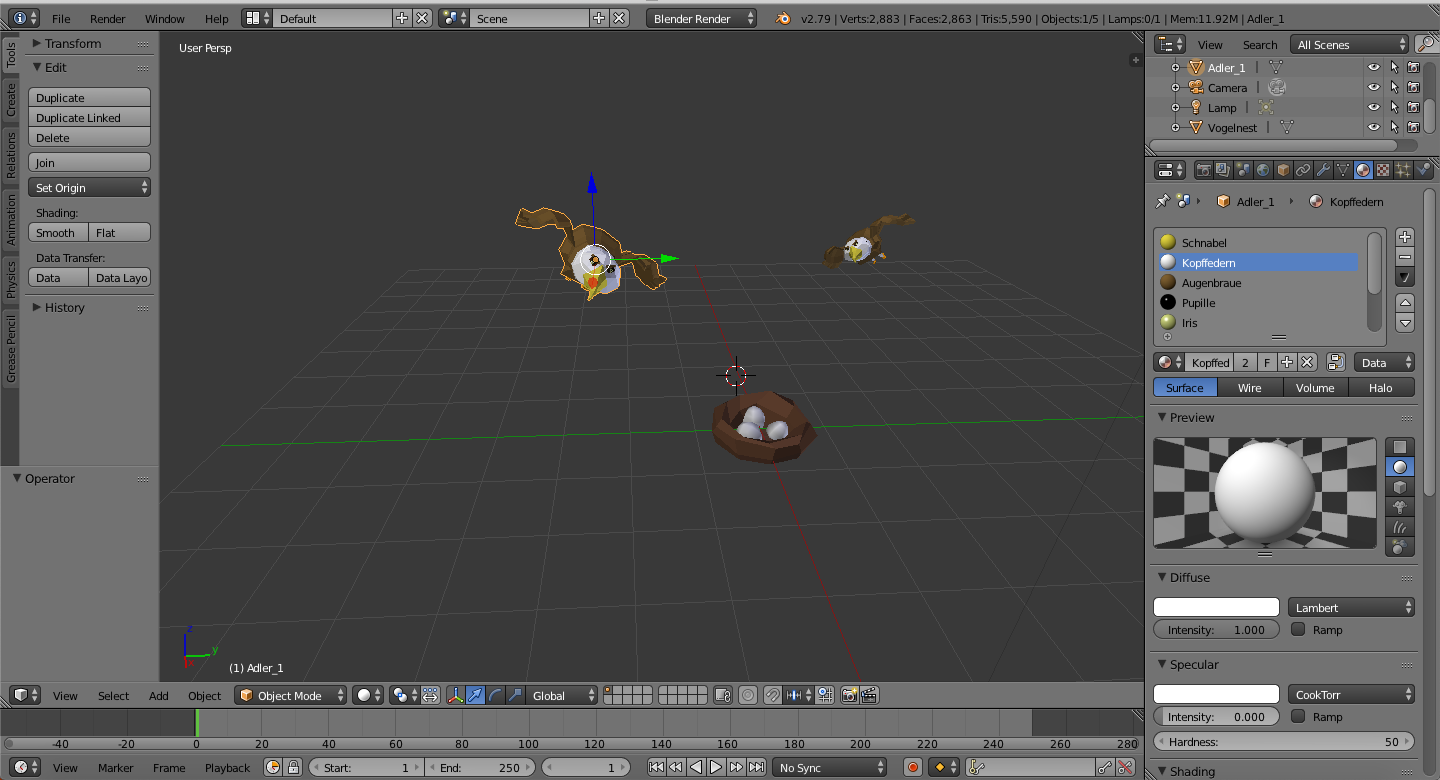
\includegraphics[width = 16cm, height = 9cm]{Blender_Foto.png}
\caption{Blenderoberfläche bei der Erstellung von 3D-Modellen für die Appliaktion}
\label{fig:Blender}
\end{figure} 

 \subsection{Unity}
Unity ist eine  Laufzeit- und Entwicklungsumgebung für Spiele, die vom Unternehmen Unity Technologies entwickelt worden ist. Unity bietet Funktionen, die schon seit langem von Unternehmen für professionelle Visualisierungen genutzt werden. Im Rahmen dieser Arbeit bietet Unity die Schnittstelle für die Nutzung der Microsoft HoloLens und den erstellten Animationen (Blender). Des Weiteren wird über Unity ein Userinterface für die Durchführung der Versuche entwickelt, welches die Effektivität bei der Durchführung der Versuche steigern soll. 

  \begin{figure}[H]
\centering
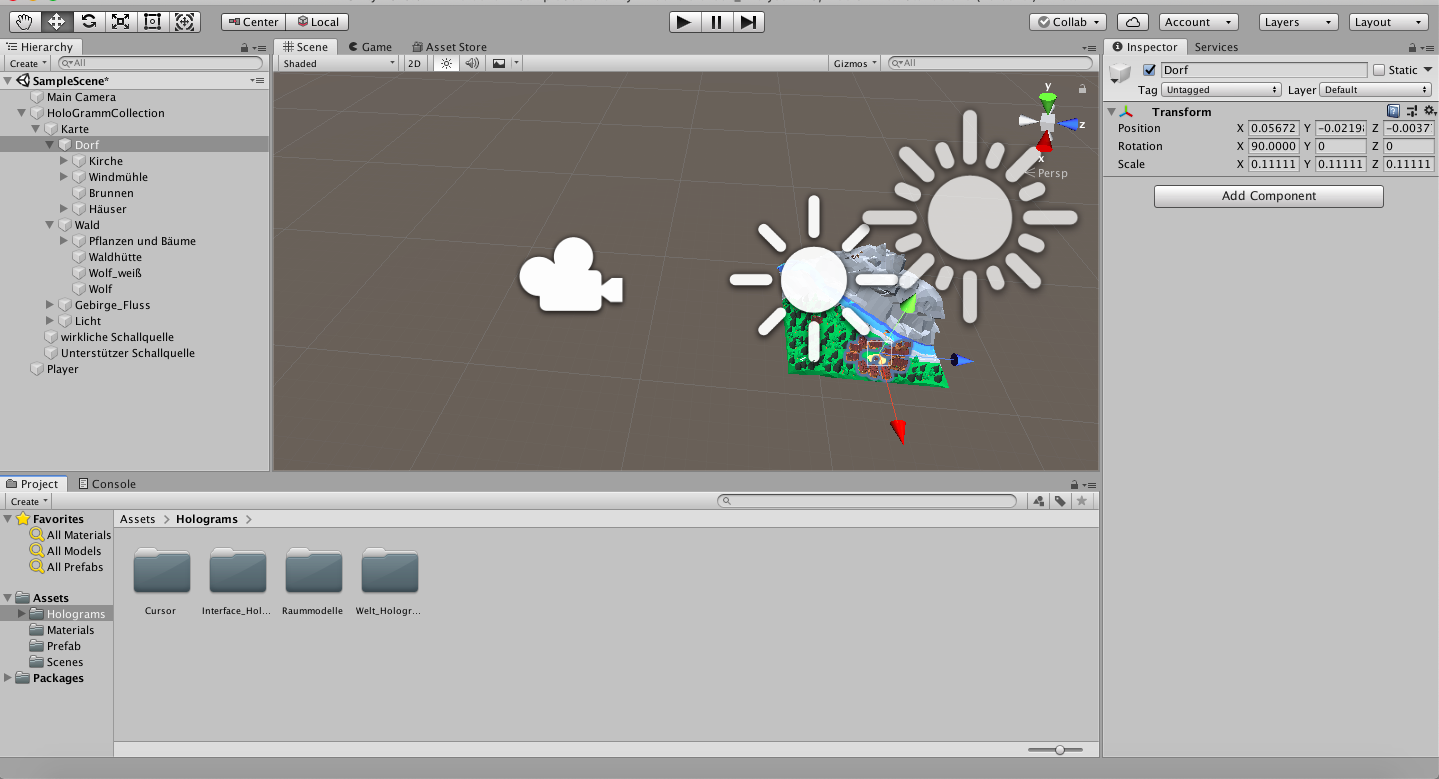
\includegraphics[width = 16cm, height = 9cm]{Unity_Foto.png}
\caption{Unityoberfläche bei der Erstellung der Appliaktion}
\label{fig:Unity}
\end{figure} 


\chapter{Vorstellung der HoloLens-Applikation und des Hörversuches}

Ziel dieser Arbeit ist es zu überprüfen wie gut bei VR- und AR-Anwendung virtuelle Schallquellen mit räumlichem Audio lokalisiert werden können und wie 3D-Audio bei solchen Anwendungen allgemein angenommen wird. Hierfür wurde ein Hörversuch in einer Mixed-Reality-Umgebung durchgeführt. Die dafür verwendete HoloLens-Applikation wurde mit Unity entwickelt. Im folgenden sollen die App und der Versuchsaufbau vorgestellt werden. 


 \section{Idee hinter dem Versuch}
 
 Bei dem im Hörversuch nachgestellten Szenario handelt es sich um einen typischen Anwendungsfall für Augmented Reality. Über das Head-Up-Display der HoloLens werden virtuelle Objekte auf einen Tisch vor dem Nutzer projiziert. In der Industrie findet sich so ein Anwendungsfall zum Beispiel in der Vorstellung von virtuellen Prototypen. Für die Vorstellung solcher Prototypen wird neben dem Visuellen auch die auditive Komponente immer wichtiger. 
 
 Hierbei wird von Software, wie z.B Unity, die Möglichkeit geboten virtuelle Schallquellen an bestimmten Positionen im Raum zu platzieren. Diese sollen dann nach Möglichkeit so klingen als wären diese tatsächlich an der angegeben Position im Raum.  Bei der Vorstellung eines Motorprototypen über AR könnte so z.B eine visuelle aber auch akustische Kostprobe gegeben werden. 
 
 Wie plausibel diese Tools virtuelle Schallquellen in den Raum projizieren und ob die Konsumenten diese Darbietung überhaupt so annehmen wie gewünscht, soll anhand eines Hörversuches ermittelt werden. 
 
 \newpage
 \section{Beschreibung der Virtuellen Welt}
 
 In dem Versuch wird eine virtuelle Welt im lowpoly-Grafikstil auf einen Tisch vor den Probanden projiziert. Es handelt sich hierbei um eine  Landschaft mit einem Gebirge, einem Fluss, einem Dorf und einem Waldgebiet. Die Welt ist ca. 1m breit wie tief und bis zu 70cm hoch. Im Folgenden werden die einzelnen Gebiete genauer beschrieben. Die dort platzierten Hörereignisse werden in einem einzelnen Kapitel vorgestellt. 
 
 \begin{figure}[H]
\centering
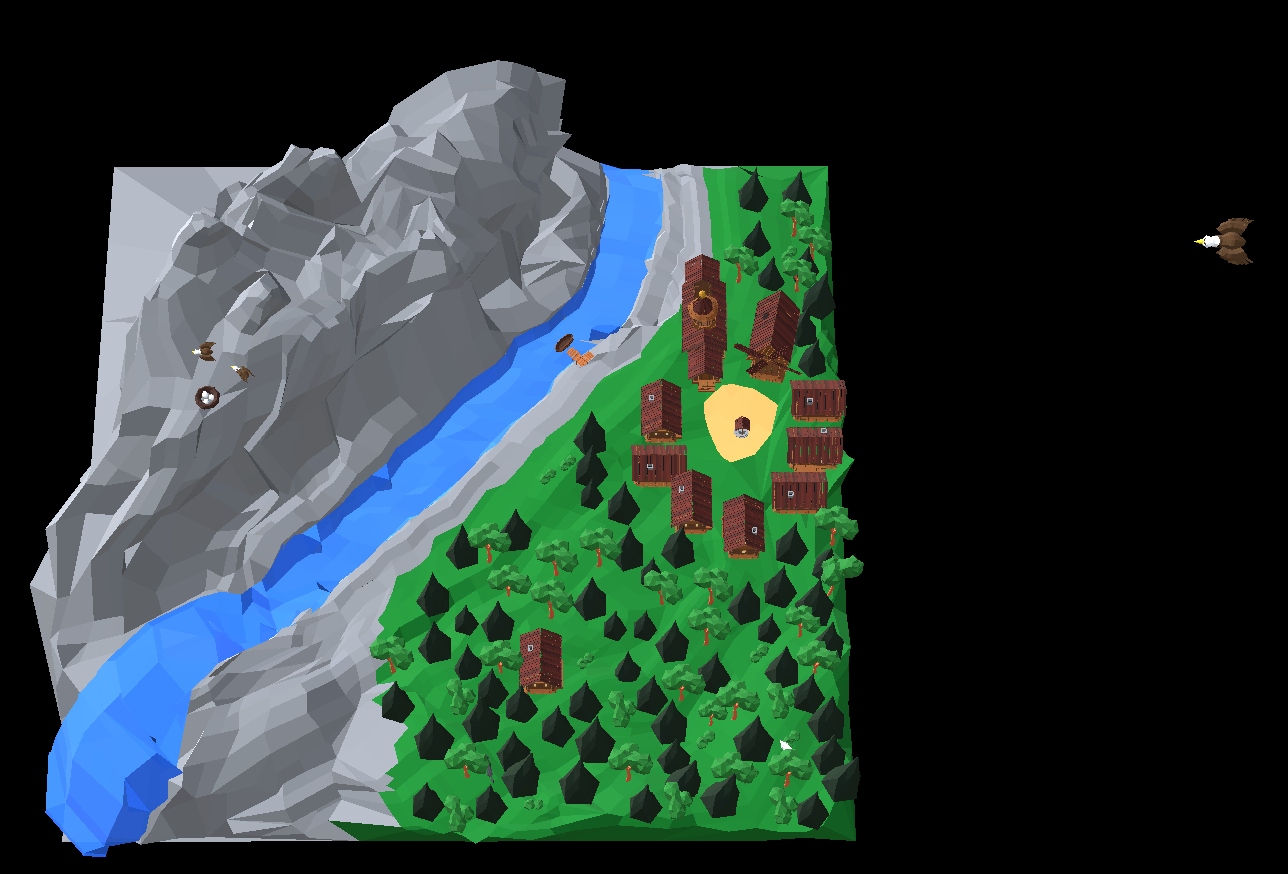
\includegraphics[width = 15cm, height = 8cm]{Komplette_welt_Draufsicht.png}
\caption{Hologramm der virtuellen Welt von oben}
\text{Rechts, über der Welt und dem Probanden, befindet sich zusätzlich ein weiterer Adler.}
\label{fig:Draufsicht}
\end{figure} 

\subsection{Dorf}
Das Dorf befindet sich am Rand des Waldes und wird durch den Fluss vom Gebirge abgetrennt. Im Zentrum des Dorfes befindet sich ein Brunnen, der auf einer Sandfläche steht. Darum herum sind sieben einfache Häuser, sowie eine Mühle und eine Kirche platziert. Die Kirche besitzt einen Glockenturm mit einer großen, goldenen Glocke. Diese könnte als potentielle virtuelle Schallquelle verwendet werden, wobei das Hörereignis der erschallenden Kirchenglocken ohne räumliches Audio wiedergegeben wird und somit keine Position in der Welt einnimmt. \\

TODO: Besseres Bild machen. 

 \begin{figure}[H]
\centering
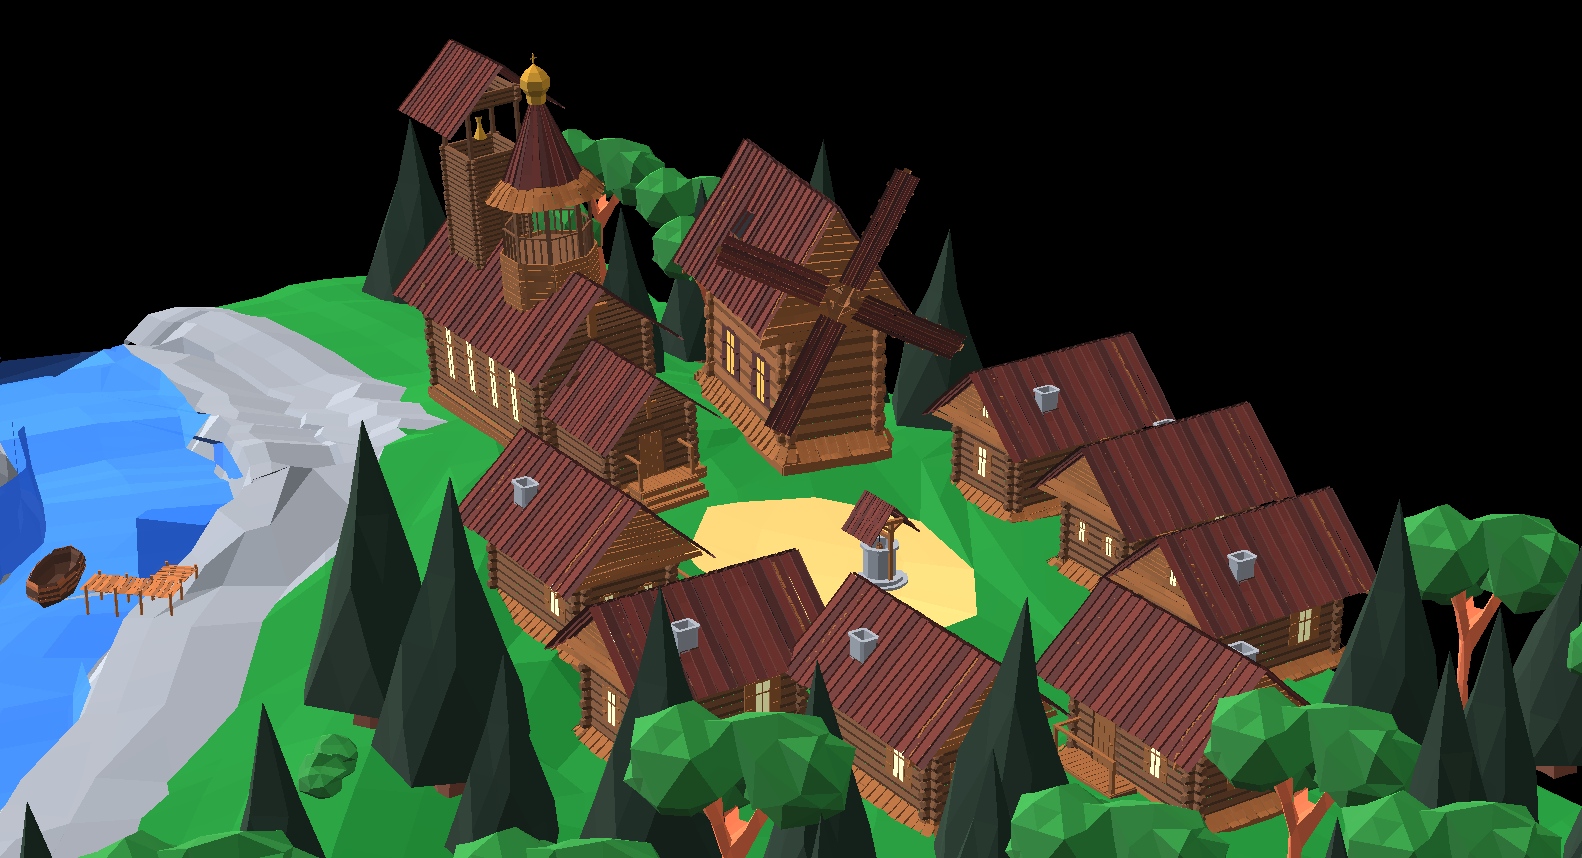
\includegraphics[width = 15cm, height = 8cm]{Dorf.png}
\caption{Dorf: Die Kirchenglocke dient als Ort für potentielle Schallquelle}
\label{fig:Dorf}
\end{figure} 

\subsection{Wald}
Der Wald besteht aus zum größten Teil aus Pflanzen und Bäumen. Im Wald befindet sich noch ein einfaches Haus und zwei Wölfe, wobei einer weiß und einer grau ist. Zu Beginn des Hörversuchs befindet sich der Wald im Vordergrund. Der weiße Wolf sticht hierbei durch seine Farbe, seine Größe und seine Position heraus, während der graue Wolf zunächst eher durch Bäume und Büsche verdeckt wird. Eine virtuelle Schallquelle wird an der Position des grauen Wolfes platziert. 

 \begin{figure}[H]
\centering
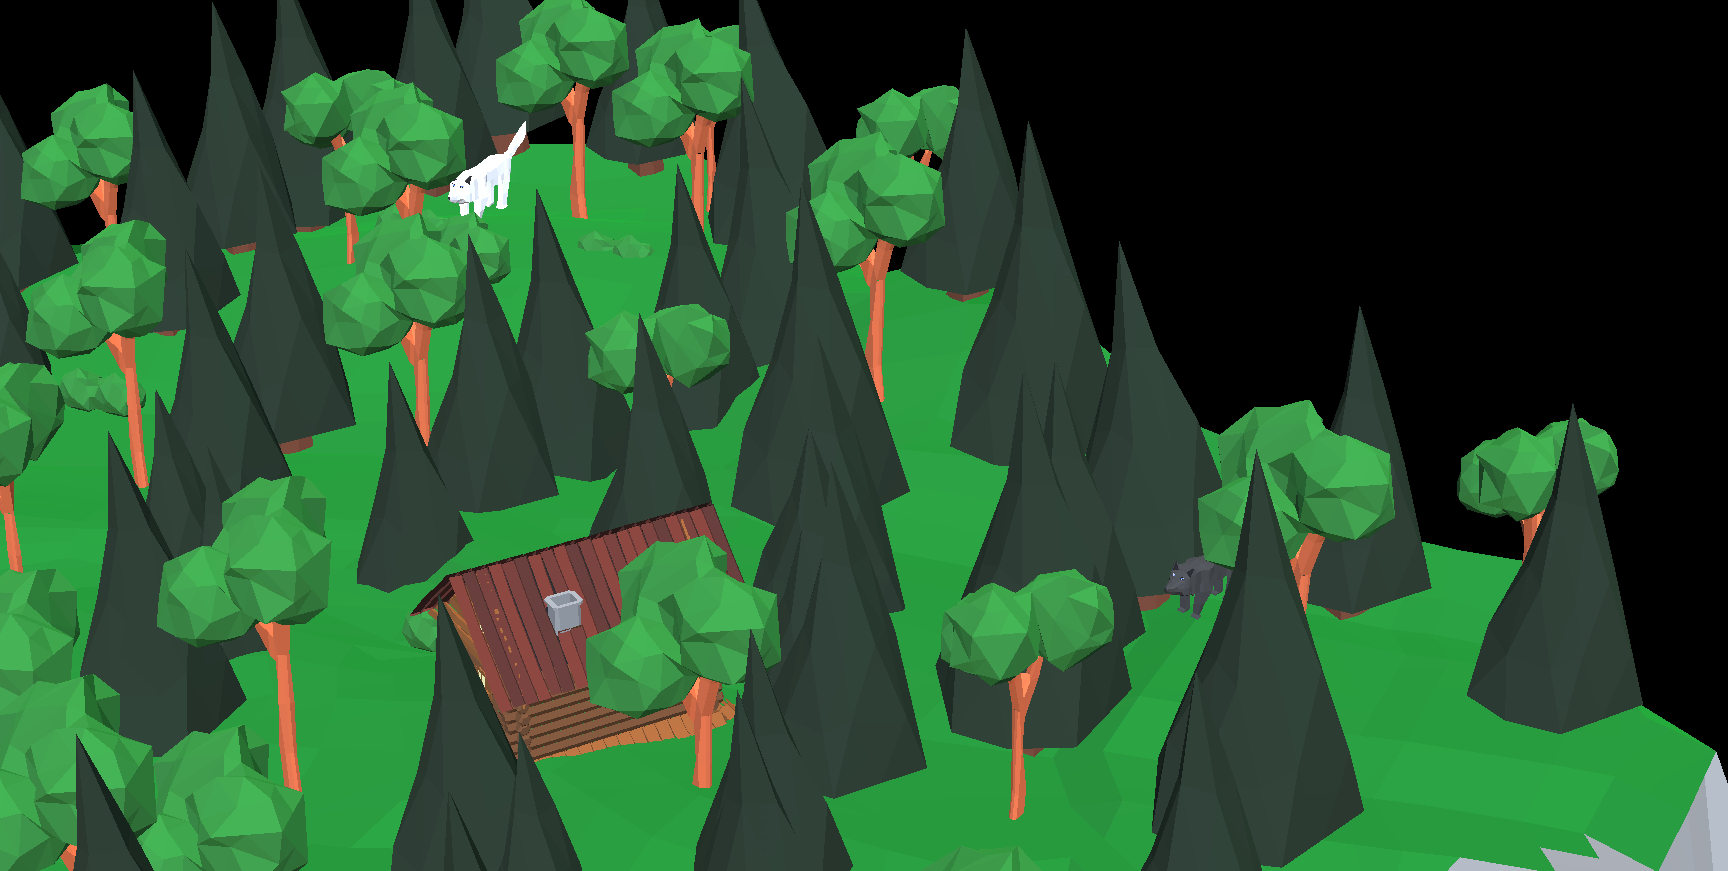
\includegraphics[width = 15cm, height = 8cm]{Wald.png}
\caption{Wald: Schwarzer Wolf dient als Ort für Schallquelle}
\label{fig:Wald}
\end{figure} 

\subsection{Gebirge und Fluss}
Das Gebirge ist das höchste Gebiet der Welt und wird vom Fluss von der restlichen Welt abgegrenzt. Die Bergspitze des größten Berges ist hierbei ca. 70cm hoch. In dem Gebirge befindet sich ein Adlernest, über dem zwei Adler fliegen. Eine virtuelle Schallquelle wird im Adlernest platziert. 

   Ein weiterer Adler befindet sich weit über der Welt, über dem Probanden. An dieser Position befindet sich ebenfalls eine virtuelle Schallquelle. Diese spielt das gleiche Signal ab wie die virtuelle Schallquelle im Adlernest, siehe Abbildung \ref{fig:Draufsicht}. 

Am Fuße des Gebirges befindet sich ein Fluss. Dieser fließt von einer erhöhten Quelle abwärts in Richtung des Dorfes und geht hierbei von einem Kante der Karte bis zur gegenüberliegenden. 

An der Stelle wo der Fluss an das Dorf angrenzt befindet sich ein Steg mit einem kleinen Boot. Eine virtuelle Schallquelle wird an der Quelle des Flusses platziert und eine weitere im Boot. Beide virtuellen Schallquellen spielen das gleiche Audio-Signal ab. 

 \begin{figure}[H]
\centering
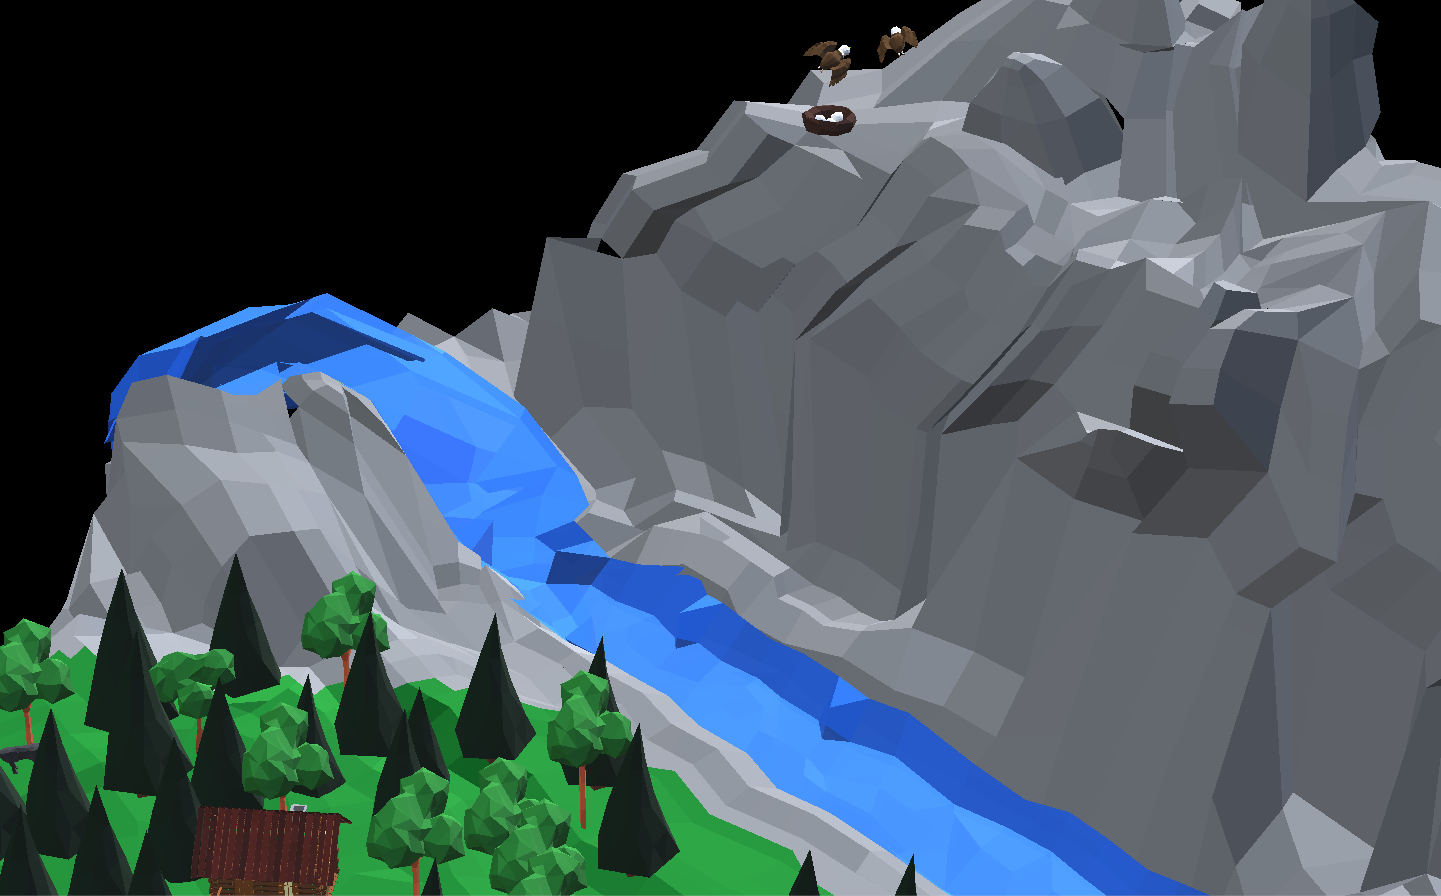
\includegraphics[width = 15cm, height = 8cm]{Gebirge_Fluss.png}
\caption{Gebirge und Fluss: Adler, Adlernest und Fluss dienen als  Ort für Schallquellen}
\label{fig:GebirgeFluss}
\end{figure}
   
  
   
    \section{Audio-Einstellungen in der Applikation}
    Die virtuelle Schallquelle ist in Unity ein Audio Source - Objekt. Die Einstellungen für das Audio Source Objekt sind nach dem Microsoft Tutorial für Spatial Audio für Mixed Reality vorgenommen worden \cite{MSSpatialAudio}. Diese Einstellungen gelten im Folgenden als Standart-Einstellungen. Abweichungen der Einstellungen werden in den Beschreibung für die Einzelszenen genannt.  Bei den abgespielten Audio-Signalen handelt es sich ausschließlich um MP3 codierte Geräusche die mit 48 kHz abgetastet werden. 
 
   TODO: Bild der Einstellungen aus Unity-Screenshot oder Liste ausführen 
   \begin{description}
\item[Update Intervall:] 0.15 
\item[Max Distance:] 20
\item[Max Objects:] 10
\end{description}


   \subsection{Binauralisierung in der Applikation}
   
Für das räumliche Audio wird der MS HRTF Spatializer und damit ein einheitlicher HRTF-Datensatz verwendet. Der MS HRTF Spatializer berechnet für die Szene jeweils die benötigten kopfbezogenen Übertragungsfunktionen für jedes Ohr des Probanden. Auf diese Weise gelingt eine binaurale Wiedergabe der Audio-Signale über die Kopfhörer der HoloLens. 

\subsection{Auralisierung in der Applikation}

Für eine plausible Wiedergabe wird eine Anpassung der Geräusche an den Versuchsraum mittels "Microsoft Spatial Audio" vorgenommen. Hierfür wird ein abstraktes Raummodell des Versuchsraumes entworfen und in die Unity-Szene integriert \ref{fig:Raummodell}. Dem Raummodell wird anschließend ein "Audio Occluder"-Script hinzugefügt. Microsoft empfiehlt in seinem Tutorial bei den Parametern des "Audio Occluders" eine Tiefpass-Grenzfrequenz von 1500Hz und eine Lautstärkereduzierung um den Faktor 0.75 einzustellen, um plausiblen diffusen Nachhall zu imitieren\cite{MSSpatialAudio}.
 
  \begin{figure}[H]
\centering
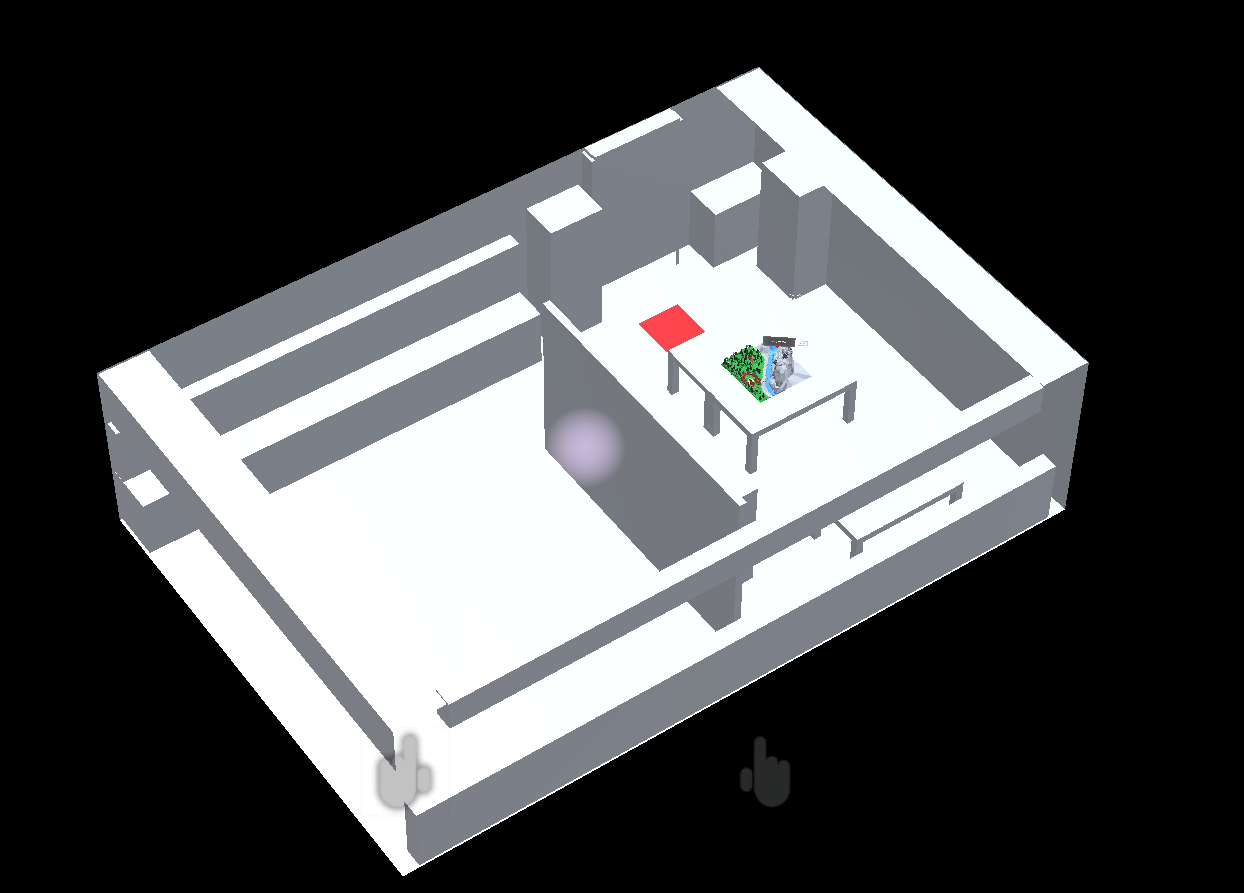
\includegraphics[width = 15cm, height = 8cm]{Raummodell_2.png}
\caption{Abstraktes Raummodell des Versuchsraumes E113 der HS Emden/Leer}
\label{fig:Raummodell}
\end{figure} 

Jedem Objekt mit einer Audio Source muss zusätzlich ein Audio Emitter zugewiesen werden. Die Parameter der Emitter werden wie folgt festgelegt: 

\begin{description}
\item[Update Intervall:] 0.15 
\item[Max Distance:] 20
\item[Max Objects:] 10
\end{description}

Durch die gewählten Parameter wird alle 0.15 Sekunden eine Neuberechnung der Raumakustik vorgenommen, was für die langsamen Bewegungen des menschlichen Kopfes genügen sollte.  Zusätzlich werden nur maximal 10 Objekte das Audio-Signal beeinflussen können. Diese dürfen dabei eine Distanz von maximal 20m entfernt sein.  Auf diese Art und Weise kann sichergestellt werden, dass die Anpassung der Audio-Signale einen natürlichen Klang hervorbringt. 

  \section{Beschreibung der Szenen des Hörversuchs}
  Der Hörversuch umfasst fünf verschiedene Szenen. In jeder Szene gibt es ein Hörereignis, das der Proband zu lokalisieren hat. Die Welt ist statisch und verändert sich während des Versuches nicht. Die virtuelle Schallquelle wird für jede Szene neu positioniert. 

  \subsection{Szene 1 - Adlerschrei im Gebirge}
  In der ersten Szene befindet sich die virtuelle Schallquelle im Adlernest, mitten im Gebirge. Bei dem Geräusch handelt es sich um das Schreien eines Adlers. Die Einstellungen weichen nicht vom gewählten Standard ab. 
  
    \begin{figure}[H]
\centering
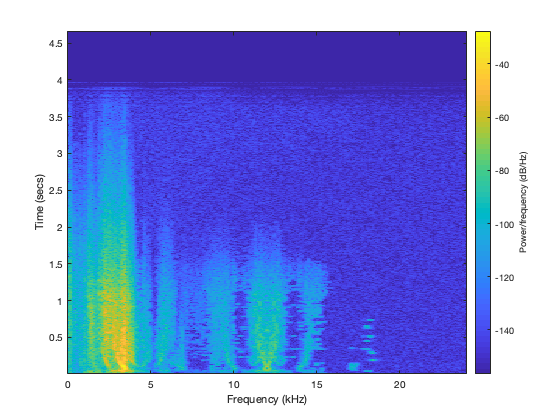
\includegraphics[width = 15cm, height = 10cm]{Adler_Spektogramm.png}
\caption{Spektorgramm des Adlergeschreis}
\label{fig:Adler_Spektogramm}
\end{figure} 

Abbildung \ref{fig:Adler_Spektogramm} zeigt das Spektogramm des Adlergeräusches. Es ist zu erkennen, dass das Geräusch ein breites Frequenzspektrum besitzt, jedoch die meisten Frequenzen zwischen 2 und 4 kHz liegen. Über den zeitlichen Verlauf lässt sich sagen, dass das Signal sich vor allem durch ein kurzes intensives Geräusch am Anfang auszeichnet, dass im Frequenzbereich zwischen 2 kHz und 4 kHz noch einige Sekunden ausklingt während die höheren Frequenzen schneller nachlassen.\\

 Der Schrei eines Adlers ist ein Geräusch, dass vermutlich jedem Probanden aus Fernsehen oder anderen Medien bekannt sein sollte. Gleichzeitig werden die meisten Probanden diesem Geräusch vermutlich noch nie in ihrem echten Leben begegnet sein.

\subsection{Szene 2 - Wolfsheulen}

In der zweiten Szene befindet sich die virtuelle Schallquelle auf dem grauen Wolf im Wald. Das Geräusch beinhaltet das Heulen eines einsamen Wolfes. Das Spezielle an der Szene ist, dass es im unmittelbaren Blickfeld des Probanden eine alternative, potentielle Schallquelle mit dem weißen Wolf gibt. Dieser wird in der Regel vom Betrachter auf Grund seiner Größe, seiner Erscheinung und seiner ungeschützten Position leichter entdeckt. Interessant wird es daher zu beobachten, ob die Probanden in der Lage sind, auf Grund des Geräusches,  den schwarzen Wolf zu erblicken und diesen als virtuelle Schallquelle zu bestimmen.  Die Einstellungen für die Wiedergabe weichen erneut nicht vom gewählten Standard ab. 

 \begin{figure}[H]
\centering
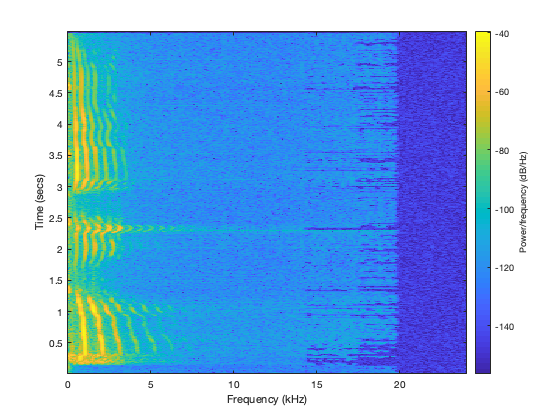
\includegraphics[width = 15cm, height = 10cm]{Wolf_Spektogramm.png}
\caption{Spektorgramm des Wolfsheulens}
\label{fig:Wolf_Spektogramm}
\end{figure} 

In Abbildung \ref{fig:Wolf_Spektogramm} ist das Spektogramm des Wolfsheulen zu sehen. Es ist zu erkennen, dass es sich in regelmäßigen, zeitlichen Intervallen auf ähnliche Art und Weise wiederholt. Das Geräusch besteht hauptsächlich aus Frequenzen zwischen 1 Hz und 5 kHz. Auffällig ist dabei, dass es zur Bildung schmaler Frequenzkeulen kommt, die sich bei vielfachen Frequenzen wiederholen. Es ist daher anzunehmen, dass sich das Geräusch harmonisch anhört. \\

Das Heulen eines Hundes könnte aufgrund der Verbundenheit des Menschen zu ihren Hunden ein Gefühl von Empathie auslösen. Wird das Geräusch eher als Wolfsheulen wahrgenommen, so könnte dieses Geräusch eher ein Angstgefühl beim Probanden bewirken. In beiden Fällen sollte das Geräusch ein befremdliches Gefühl auslösen und nicht als angenehm empfunden werden. 


\subsection{Szene 3 - Kirchenglocken}
Das Erklingen von Kirchenglocken in der dritten Szene wird ohne räumliches Audio durchgeführt und soll mit als Referenz dienen. Aus diesem Grund gibt es in dieser Szene keine virtuelle Schallquelle mit festgelegter Position. Es ist bei dieser Szene zu beobachten, ob die Probanden die Darbietung trotz des fehlenden, räumlichen Audios als plausibel und angenehm empfinden. Außerdem stellt sich die Frage, ob die Schallquelle rein auf Grund der visualisierten Kirchenglocke auch dort von den Probanden lokalisiert werden wird.
 
    \begin{figure}[H]
\centering
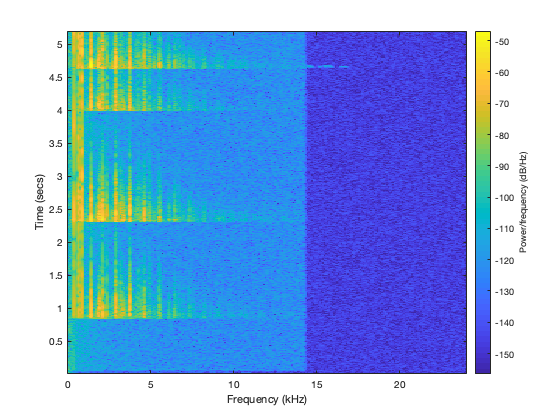
\includegraphics[width = 15cm, height = 10cm]{Kirchenglocken_Spektogramm.png}
\caption{Spektorgramm der Kirchenglocken}
\label{fig:Kirchenglocken_Spektogramm}
\end{figure} 

Anhand Abbildung \ref{fig:Kirchenglocken_Spektogramm} lässt sich erkennen, dass das Geräusch der erklingenden Kirchenglocken ebenfalls eindeutige Frequenzkeulen aufweist, die sich bei vielfachen Frequenzen wiederholen. Aus diesem Grund handelt es sich ebenfalls um ein harmonisches Klangereignis. Das Frequenzspektrum umschließt Frequenzen zwischen 100 Hz und 10 kHz, wobei besonders die tiefen Frequenzen zwischen 100 Hz und 1kHz sehr dominant sind. \\

Zeitlich verhält sich sich das Audio-Signal so, dass es immer zu einem  wiederholenden Anschlag der Glocken neu ertönt. Hierbei lassen die hohen  Frequenzen ebenfalls schneller nach als die tieferen. Besonders auffällig ist dabei, dass die sehr tiefen Grundtöne zwischen zwei Glockenschlägen nicht vollends abklingen, so dass diese Frequenzen dauerhaft zu hören sind.  \\

Das erklingen von Glocken sollte in der Regel als angenehmes Geräusch wahrgenommen werden und wird häufig auch mit einem Friedensgefühl assoziiert. 

\subsection{Szene 4 - Flussrauschen}
In der vierten Szene  des Hörversuchs werden im Vergleich zu den anderen Szenen zwei virtuelle Schallquellen im Raum platziert, die beide das gleiche Geräusch wiedergeben. Bei diesem handelt es sich um das Rauschen eines Flusses. Eine virtuelle Schallquelle wird hierbei an der Quelle des Fluss, im Gebirge und eine neben dem Boot, am anderen Ende des Flusses platziert. Je nach Position des Probanden dürfte sich eine Phantomschallquelle entweder zwischen den beiden Schallquellen  oder an der nächstgelegenen Schallquelle bilden. 

 \begin{figure}[H]
\centering
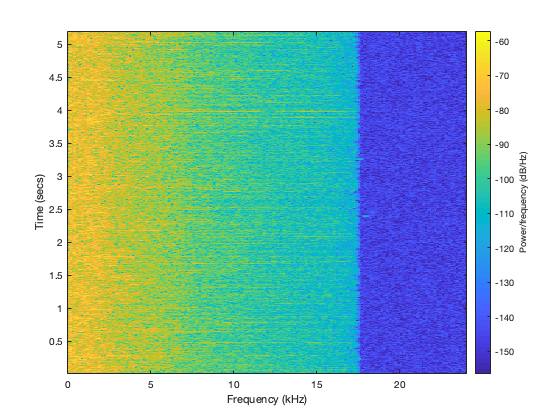
\includegraphics[width = 15cm, height = 10cm]{Fluss_Spektogramm.png}
\caption{Spektorgramm des Flussrauschens}
\label{fig:Fluss_Spektogramm}
\end{figure} 

Das Spektogramm des Flussrauschens in Abbildung \ref{fig:Fluss_Spektogramm} ähnelt sehr dem eines rosa Rauschens. Von den tiefen zu den hohen Frequenzen nimmt die Intensität ab. Die beruhigende Wirkung von rosa Rauschen könnte dementsprechend  auch dem Flussrauschen zugesprochen werden. \\ 

Auch inhaltlich sollte das Rauschen eines Flusses eher als angenehm wahrgenommen werden. 

\subsection{Szene 5 - Adlerschrei über der Welt}
In der letzten Szene wird die virtuelle Schallquelle bei dem Adler über dem Probanden platziert. Das Geräusch ist hierbei das selbe wie bei der ersten Szene. \\ 

In der Realität handelt es sich bei dem Adlerschrei um eine Geräusch, dass eigentlich über dem Hörenden erwartet wird. Dadurch, dass sich das Geräusch nun tatsächlich über dem Probanden befindet müsste es eigentlich ein plausibles Hörereignis darstellen. Es bleibt jedoch abzuwarten ob die Probanden anhand des Schalls den Adler über sich überhaupt lokalisieren können oder ob die offensichtlicheren Adler im Gebirge von der eigentlichen virtuellen Schallquelle ablenken.  

 \section{Bewertungskriterien der Darbietung}
 Zur Bewertung der Darbietung werden dem Probanden Fragen zum Darbietungsempfinden gestellt. Dieser hat der Proband mit Hilfe von jeweils  zwei dualistischen  Antwortmöglichkeiten zu beantworten. Dabei kann der Proband in zehn Stufen einordnen, welche der beiden Antworten für ihn eher zu trifft. Diese Art der Befragung erlaubt es den Probanden bei der Bewertung ihren Freiraum zu lassen, aber gleichzeitig die Probandendaten untereinander vergleichbar zu machen.  \\
 
 Mit Hilfe der Fragen soll herausgestellt werden, ob der Proband die Szene als plausibel wahrnimmt, inwiefern bei ihm ein Immersionsgefühl zustande kommt und ob er sich bei der Darbietung wohlgefühlt hat. \\
 
 Wird eine Szene als plausibel bezeichnet, dann bedeutet dies, dass die Summe aller Sinneseindrücke für den Betrachter glaubhaft und nachvollziehbar ist. Dies wird vor allem dann erreicht wenn die Sinneseindrücke natürlich wirken und den Konsumenten nicht verwirren. \\
 
 Ein wichtiges Kriterium für Plausibilität ist, dass die wichtigsten Sinneseindrücke, also das Gehörte und das Gesehene, zusammen passen. Ist beispielsweise ein Hörereignis ohne ersichtlichen Grund weit von der Schallquelle entfernt, dann widerspricht dies dem natürlich Verständnis des Menschen für Kausalität. Mit der ersten Frage soll daher geprüft werden, ob für den Probanden das Visuelle und das Auditive plausibel zusammenarbeiten.\\
 
 Ein weiteres Kriterium Plausibilität ist der Realismus der Sinneseindrücke. Hierbei geht es weniger darum, dass visuelle und auditive Reize als komplett realistisch wahrgenommen werden, sondern vielmehr darum, dass diese sich in das Gesamtbild einfügen. Da das Visuelle in dem Hörversuch auf einem Low-Poly-Grafikstil basiert, wird niemand von den Geräuschen absoluten Realismus erwarten. Wichtig ist jedoch trotzdem, dass die Geräusche als Komponente der unmittelbaren Umgebung wahrgenommen werden, anstatt als alleinstehendes Audio-Signal, welches über die Kopfhörer wiedergegeben wird. Die zweite Frage soll daher Klarheit darüber geben, inwiefern die Probanden die Geräusche als realen Bestandteil ihrer Umgebung wahrnehmen. \\
 
Bei der Erstellung von AR- und VR-Anwendungen ist das Wohlbefinden des Konsumenten  ein zu beachtender Faktor. Das stärkere Immersionsgefühl bei AR und VR ermöglicht es noch realistischere, mediale Inhalte zu erstellen. Dies setzt aber auch voraus darauf zu achten unter welchen Umständen sich der Konsument wohlfühlt. Mit der Entdeckung des Uncanny Valley wurde bereits bewiesen, dass zu realistische visuelle Reize Unwohlsein auslösen können. Inwiefern dies auch mit dem steigernden Realismus von räumlichem Audio bewirkt werden könnte ist noch nicht vollends erforscht. Aus diesem Grund soll mit der dritten Frage das Wohlbefinden des Probanden während der Darbietung überprüft werden. 
 
 \begin{figure}[H]
\centering
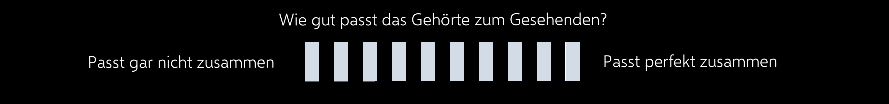
\includegraphics[width = 16cm, height = 2cm]{Frage1.png}
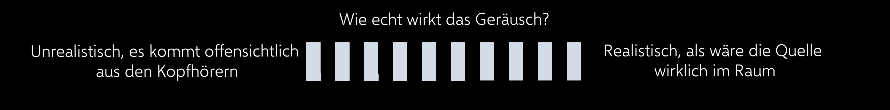
\includegraphics[width = 16cm, height = 2cm]{Frage2.png}
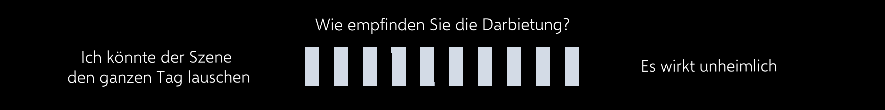
\includegraphics[width = 16cm, height = 2cm]{Frage3.png}
\caption{Fragen zur Bewertung der Szenen im Hörversuch}
\label{fig:Fragen}
\end{figure} 

Anhand der Bewertungen des Probanden soll ermittelt werden, wie stark das Immersionsgefühl bei der Darbietung der Szenen gewesen ist. Dabei wird davon ausgegangen, dass die gewichtete Antwort der ersten beiden Fragen mit dem Immersionsgefühl des Probanden korreliert. Nimmt ein Proband das Geräusch als Teil des Raumes war und empfindet gleichzeitig das Zusammenspiel aus Visuellem und Auditivem als plausibel, dann ist auch davon auszugehen, dass das Immersionsgefühl des Probanden recht intensiv ist. Auf diese Weise kann überprüft werden bei welcher Szene das stärkste Immersionsgefühl bewirkt wird. \\ 

Im Zweifel wegfallen lassen: Um das Immersionsgefühl statistisch erfassen zu können, wird der Durchschnitt der gewichteten Antworten für die ersten beiden Fragen im Folgenden als Immersionsgefühl festgehalten. \\

Die zu Anfang gestellte These, dass es eine Art Uncanny-Valley-Effekt für zu realistisches Audio geben könnte, soll anhand der Versuchsergebnisse ebenfalls überprüft werden. . Lässt sich ein Zusammenhang zwischen dem Immersionsgefühl bzw. dem bewerteten Realismus der Szene aus Frage 2 und dem geprüften Wohlbefinden aus Frage 3 beobachten, so könnte dies Aufschluss über die gestellte These geben. Natürlich sind die durchgeführten Versuche für die Bestätigung der These nicht vollends aussagekräftig, da der Hörversuch nicht speziell auf die Erforschung dieses Themengebiets ausgelegt ist. 


 
 \section{Beschreibung der Benutzeroberfläche}
 Die Bedienung der HoloLens-App funktioniert über Head-Tracking, Gesten- und Sprachsteuerung, wobei die Probanden für den Hörversuch ausschließlich auf die Head-Tracking-Funktion und die Gestensteuerung zurückgreifen mussten. \\
 
 Mittels eines Cursors, der wie eine Computermaus funktioniert, lassen sich in der App Aktionen durchführen. Der Cursor befindet sich hierbei immer in der Mitte des Sichtfeldes des HoloLens-Nutzers. Über die Bewegung des Kopfes kann der Benutzer nun den Cursor bewegen. Der Cursor besitzt drei Darstellungsformen, um dem Nutzer seinen aktuellen Zustand zu signalisieren, siehe Abbildung \ref{fig:Cursor}. 
 
  \begin{figure}[H]
\centering
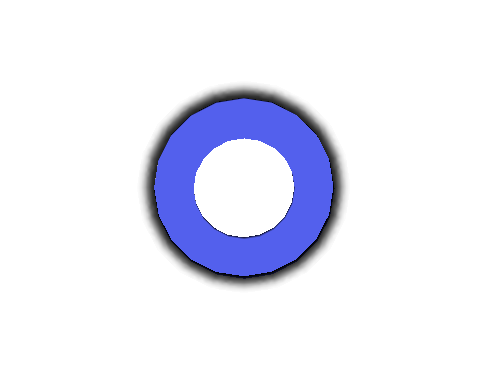
\includegraphics[width = 5cm, height = 4cm]{Cursor_default.png}
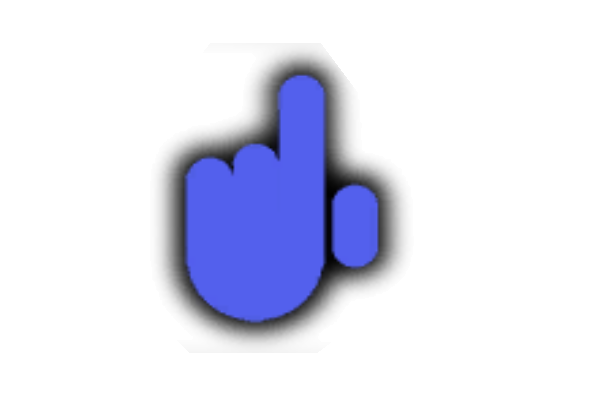
\includegraphics[width = 5cm, height = 4cm]{Cursor_Hand_Erkannt.png}
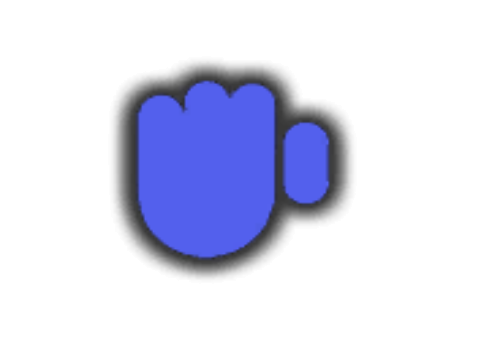
\includegraphics[width = 5cm, height = 4cm]{Cursor_Tap_Erkannt.png}
\caption{Cursor-Zustände: Default(links), Hand erkannt 
(Mitte), Tap erkannt (rechts) }
\label{fig:Cursor}
\end{figure} 
 
 Der Cursor lässt sich über Handgesten steuern. Hebt man die Hand vor sich hoch, so dass die Sensoren der HoloLens diese erkennen können, dann verändert sich der Cursor in eine Hand, siehe Abbildung \ref{fig:Cursor}. Hebt man von der geschlossen Hand aus den Zeigenfinger und drückt diesen ruckartig wieder nach unten, wird dies als Tap-Geste bezeichnet. Wurde die Tap-Geste erfolgreich von der HoloLens erkannt, dann verändert sich der Cursor erneut, siehe \ref{fig:Cursor}.   Die Tap-Geste ist ein Mittel um mit Objekten in der virtuellen Welt zu interagieren. \\
 
 Auch die Beantwortung der Fragen zur Bewertung der Darbietung gelingt über die Tap-Geste. In dem der Proband auf einen der Balken zwischen den Antwortmöglichkeiten klickt kann dieser die Szene bewerten.
 
  \begin{figure}[H]
\centering
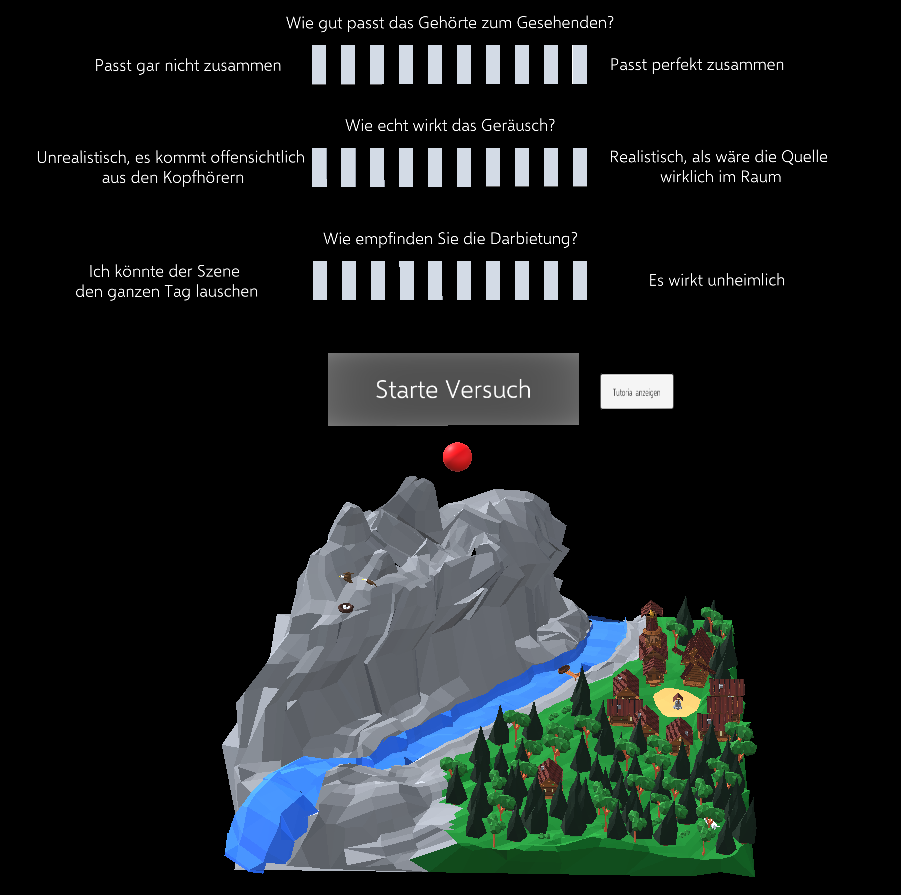
\includegraphics[width = 15cm, height = 17cm]{Welt_mit_Interface.png}
\caption{Welt mit Benutzeroberfläche und roter Kugel}
\label{fig:WeltMitInterface}
\end{figure} 
 
 
 \subsubsection{Position der Schallquelle lokalisieren}
 Eine Aufgabe des Probanden im Hörversuch ist es die Position der virtuellen Schallquelle zu lokalisieren. Damit dies spielerisch gelingt hat der Proband in der HoloLens-App die Möglichkeit eine rote Kugel dort zu platzieren, wo er denkt, dass sich die virtuelle Schallquelle befindet. Die rote Kugel befindet sich am Anfang jeder Szene direkt über der virtuellen Welt, siehe Abbildung \ref{WeltMitInterface}. Der Proband hat nun die Möglichkeit die Kugel mit dem Cursor anzuvisieren und mit der Tap-Geste die Kontrolle über die rote Kugel zu erhalten. Hat er die vermeintliche Position der virtuellen Schallquelle lokalisiert, kann er mit Hilfe der Kopfbewegung die rote Kugel dorthin schieben und mit einer weiteren Tap-Geste an der gewünschten Position platzieren. So kann der Proband leicht und sofort visualisiert angeben, wo er die Schallquelle hört. 
 
 \subsubsection{Sprachbefehle und Positionierung der Welt}
 Für die Positionierung der Welt wurden Sprachbefehle implementiert mit denen sich die Welt bewegen lässt. Mit dem Start der App befindet sich die Welt im Rotationsmodus (Sprachbefehl: "Rotate Mode"), wodurch sich die Welt mit der Tap-Geste um die Y-Achse rotieren lässt. Mit dem Sprachbefehl "Move Mode" lässt wird in den Bewegungsmodus gewechselt. In diesem lässt sich die Welt frei im Raum bewegen. Ist die gewünschte Rotation und Transformation eingestellt, so lässt sich mit dem "Lock Mode"-Sprachbefehl die Welt feststellen. Die Hörversuche sollten im "Lock Mode" durchgeführt werden, damit der Proband nicht fälschlicherweise die Welt während des Hörversuchs bewegt. Die Sprachbefehle werden den Probanden nicht beigebracht und dienen ausschließlich zur Kontrolle der Welt.
  
 \section{Ablauf des Hörversuchs}
 Zu aller erst wird die App auf der HoloLens im Versuchslabor gestartet. Wichtig dabei ist, dass beim Start der App der Träger der HoloLens sich an der durch das Raummodell festgelegten Stelle befindet. Nur dann stimmt das in Unity festgelegte Raummodell mit dem realen Versuchsraum überein, so dass ein plausibles akustisches Ergebnis durch Spatial Audio erzielt werden kann. \\
 
 Im Anschluss wird das Hologramm der Welt, mit Hilfe der Sprachbefehle, auf dem dafür vorgesehenen Tisch platziert und festgestellt. Daraufhin kann die HoloLens an den ersten Probanden übergeben werden. \\
 
Zu Beginn des Hörversuchs stellt sich jeder Proband zunächst an die vorgesehene Stelle im Raum. Damit die Ergebnisse des Hörversuchs nicht durch eine variierende Wortwahl bei der Erklärung verfälscht werden, erhalten alle Probanden die gleiche Einweisung über ein Tutorial-Fenster, welches über die HoloLens dargeboten wird.  \\

 \begin{figure}[H]
\centering
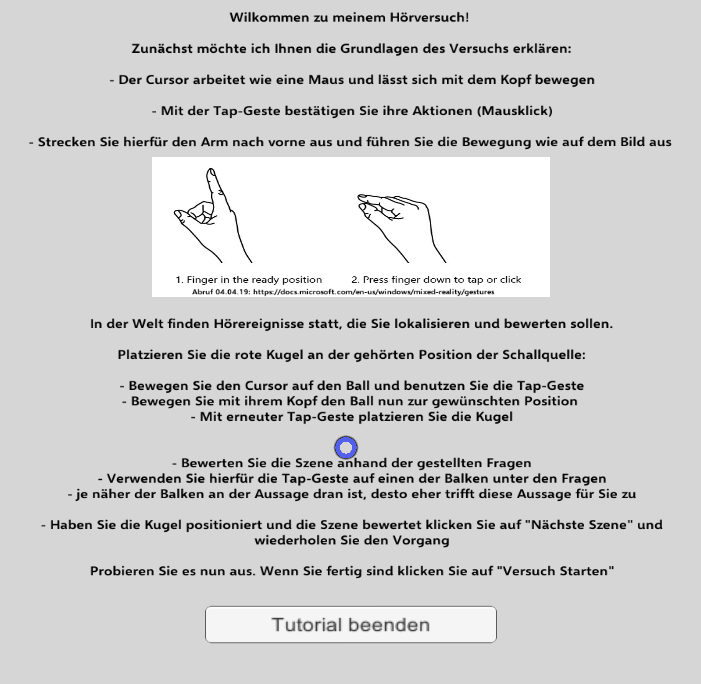
\includegraphics[width = 13cm, height = 13cm]{Tutorial.png}
\caption{Einheitliches Tutorial für die Probanden zur Erklärung der Steuerung im Hörversuch}
\label{fig:Tutorial}
\end{figure} 

Sind nach der Einweisung noch Fragen offen, so kann der Proband diese vor dem Beginn des Hörversuchs klären. Mit dem Beenden des Tutorials sieht der Proband die Welt wie in Abbildung \ref{fig:WeltMitInterface}. Hier kann der Proband testen, ob er das Tutorial verstanden hat und sowohl die Balken der Fragen markieren, als auch die Kugel im Raum platzieren.  \\
 
 Hat der Proband alles verinnerlicht ist er bereit den Hörversuch über den "Versuch starten"-Button zu starten. Daraufhin sollte das Geräusch der ersten Szene abgespielt werden. Die Aufgabe des Probanden ist es nun die rote Kugel an der Stelle zu platzieren, an der er die virtuelle Schallquelle hört und anschließend die Fragen über der Welt zu beantworten. Ist dies erledigt kann der Benutzer mit dem "Nächste Szene"-Button die nächste Szene laden. Dieser Vorgang wiederholt sich für alle fünf Szenen. Mit dem Beendigen der fünften Szene wird dem Probanden über ein Pop-Up-Fenster signalisiert, dass der Versuch abgeschlossen ist. \\
 
 Die Daten des Probanden werden für jede Szene  einzeln, lokal auf der HoloLens in einer Text-Datei gespeichert. Hierbei werden die zur Welt relativen Koordinaten und die Bewertungen als Zahlen von -5 bis 5 gespeichert. 
 
 
 \section{Probanden}
 
 Bei den für den Hörversuch ausgewählten Probanden handelt es sich hauptsächlich um Studierende der Hochschule Emden/Leer. Der Hörversuch wurde hierbei mit 17 unterschiedlichen Probanden durchgeführt, wobei leider einige aus Zeitgründen nicht alle Szenen des Versuchs durchführen konnten und vereinzelnd Probandendaten aufgrund von Bugs der App verloren gegangen sind. \\
 
  Das Alter der Probanden lag hierbei zwischen 20 und 50 Jahren, wobei die meisten zwischen 20 und 30 Jahren alt waren. Anzumerken ist hierbei, dass die abgespielten Geräusch aller eher niederfrequent waren und daher eine Beeinflussung der Ergebnisse durch das Alter in der Auswertung vernachlässigt wird. \\ 
  
 Zwölf der getesteten Personen waren männlich und drei  weiblich . Einige Probanden trugen unter der HoloLens eine Brille, dies soll aber bei der Auswertung trotz des möglichen Einflusses auf die Ergebnisse nicht weiter berücksichtigt werden. \\ 
 
 Der Hörversuch erfolgte anonym und ohne Erfassung persönlicher Daten. Die Auswertung der Probandendaten erfolgt ohne Hintergrundinformationen über die Probanden und basiert ausschließlich auf den durch die App gespeicherten Daten. Für sicherere Versuchsergebnisse sollte der Hörversuch mit einer größeren Menge an Probanden, sowie einer Erfassung der persönlichen Probandendaten, wiederholt werden.
 
 \chapter{Auswertung des Hörversuchs}
 Im Rahmen dieser Bachelorarbeit wurde ein Hörversuch mit binauralem, räumlichem Audio durchgeführt. Ziel des Hörversuches ist es herauszufinden inwiefern die natürliche Lokalisationsfähigkeit von Hörereignissen in einer Mixed Reality Umgebung gegeben ist. Bei der Durchführung des Hörversuches haben die Probanden für fünf verschiedene Audio-Szenen jeweils versucht die virtuelle Schallquelle zu lokalisieren.  Zusätzlich haben sie jeweils Fragen zum Darbietungsempfinden anhand bestimmter Kriterien beantwortet.  Die Ergebnisse des durchgeführten Hörversuches sollen im Folgenden analysiert werden.
 
 \section{Vorstellung der Versuchsergebnisse}
 Während des Versuchs hatten die Probanden für jede Szene die Aufgabe eine rote Kugel genau dort zu platzieren, wo sie die virtuelle Schallquelle anhand des Gehörten vermuteten. Die Position der roten Kugel wurde hierbei für jeden Probanden, für jede Szene dokumentiert. Es gilt nun die Daten die gesammelten Daten zu analysieren. \\
 
 Zur Visualisierung der Probandenergebnisse wird die virtuelle Welt zusammen mit der wirklichen, virtuellen Schallquelle und den von den Probanden lokalisierten, virtuellen Schallquellen dargestellt. Die echte, virtuelle Schallquelle wird, sofern es eine gibt, durch eine rosa Kugel und die von den Probanden lokalisierte virtuelle Schallquelle durch  kleinere, rote Kugeln dargestellt. Hierbei ist anzumerken, dass die Platzierung der roten Kugel aufgrund fehlender Übung mit dem Umgang der HoloLens nicht komplett genau erfolgen konnte. Es sollte daher bei der Analyse berücksichtigt werden, dass die Probanden die Kugel vielleicht nicht genau da platzieren konnten, wo sie die Schallquelle ganz genau gehört haben. 
 
 \subsection{Szene 1: Adlerschrei im Adlernest}
 In der ersten Szene wurden die in den Microsoft-Tutorials für Spatial Audio empfohlenen Einstellungen für räumliches Audio direkt übernommen. Die virtuelle Schallquelle mit dem Geschrei eines Adlers wurde für die Szene direkt in das Adlernest gelegt. Anhand der Abbildung \ref{fig:Szene_1_data} lässt sich erkennen, dass die Probanden die virtuelle Schallquellen fast ausnahmslos auf der Oberfläche des Berges neben dem fliegenden Adler unmittelbar über dem Berg lokalisiert haben. Es ist anzunehmen, dass die Probanden versucht haben die Kugel genau auf dem Adler zu platzieren und nicht im Nest, wie vorgesehen. Einige Schallquellen wurden außerdem weiter rechts im Gebirge und auch einige über dem Gebirge lokalisiert. In Abbildung \ref{fig:Szene_1_data_2} ist zu sehen, dass ein Proband die Schallquelle sogar weit über sich beim dritten Adler lokalisieren konnte. 
 
   \begin{figure}[H]
\centering
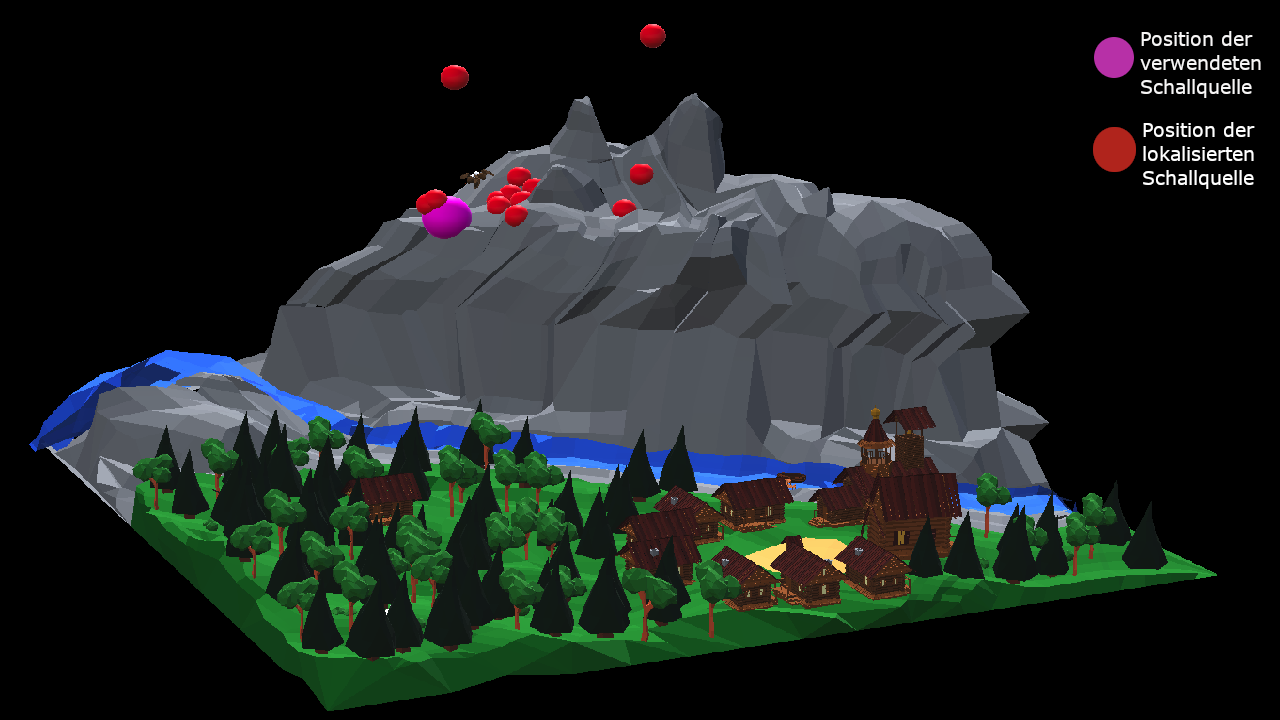
\includegraphics[width = 16cm, height = 9cm]{Szene_1_data.png}
\caption{Visualisierung der lokalisierten, virtuellen Schallquellen für Szene 1}
\label{fig:Szene_1_data}
\end{figure} 

\begin{figure}[H]
\begin{minipage}[t]{7cm}
\vspace{0pt}
\centering
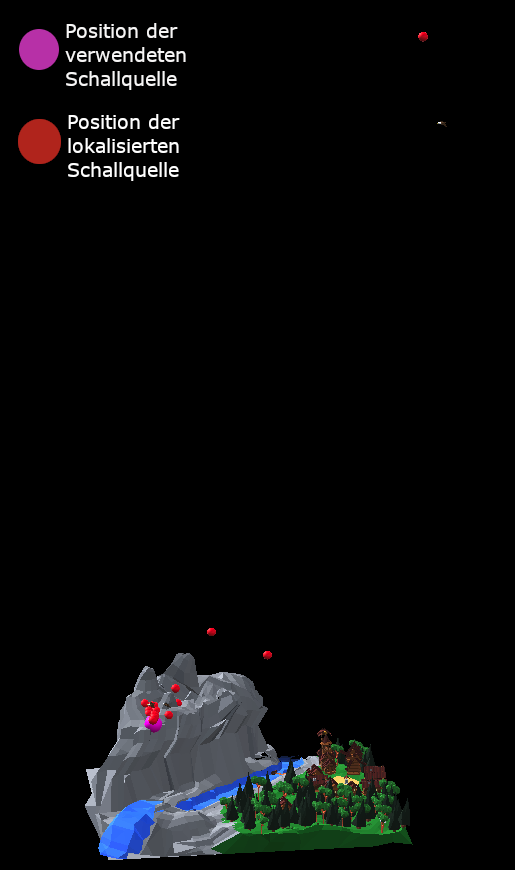
\includegraphics[width = 5cm, height = 9cm]{Szene_1_data_2.png}
\caption{Visualisierung der lokalisierten, virtuellen Schallquellen für Szene 1 aus der Seitensansicht}
\label{fig:Szene_1_data_2}
\end{minipage}
\hfill
\begin{minipage}[t]{9.5cm}
\vspace{0pt}

Anhand der Lokalisationen lässt sich erschließen, dass die Probanden zum größten Teil die ungefähre Position der virtuellen Schallquelle hören konnten. Das Wissen, dass in Wirklichkeit die Schallquelle direkt auf dem Adler liegen müsste ließ die meisten Probanden die virtuelle Schallquelle jedoch direkt auf dem Adler vermuten. Anzumerken ist jedoch, dass auch einige die Schallquelle genau richtig im Nest platziert haben, obwohl dies nicht direkt zum inhaltlichen Kontext passt. \\

Es ist ebenfalls festzuhalten, dass bis auf drei Probanden alle die virtuelle Schallquelle in der gleichen Höhe lokalisiert haben. Die Verteilung in der Horizontaltebene ist hingegen breiter verteilt. \\

Die Platzierung der Schallquelle über dem Probanden könnte ein Indiz dafür sein, dass das Visuelle einen höheren Einfluss auf die Lokalisation der Hörereignisse hat als gedacht. Obwohl der Schall eigentlich nicht so klingen sollte, als ob er von oben käme hat der Proband die Schallquelle trotzdem dort lokalisiert. Jedoch sollte berücksichtigt werden, dass es sich hierbei um einen einzelnen Ausreißer handelt.
\end{minipage}
\end{figure}


   \begin{figure}[H]
\centering
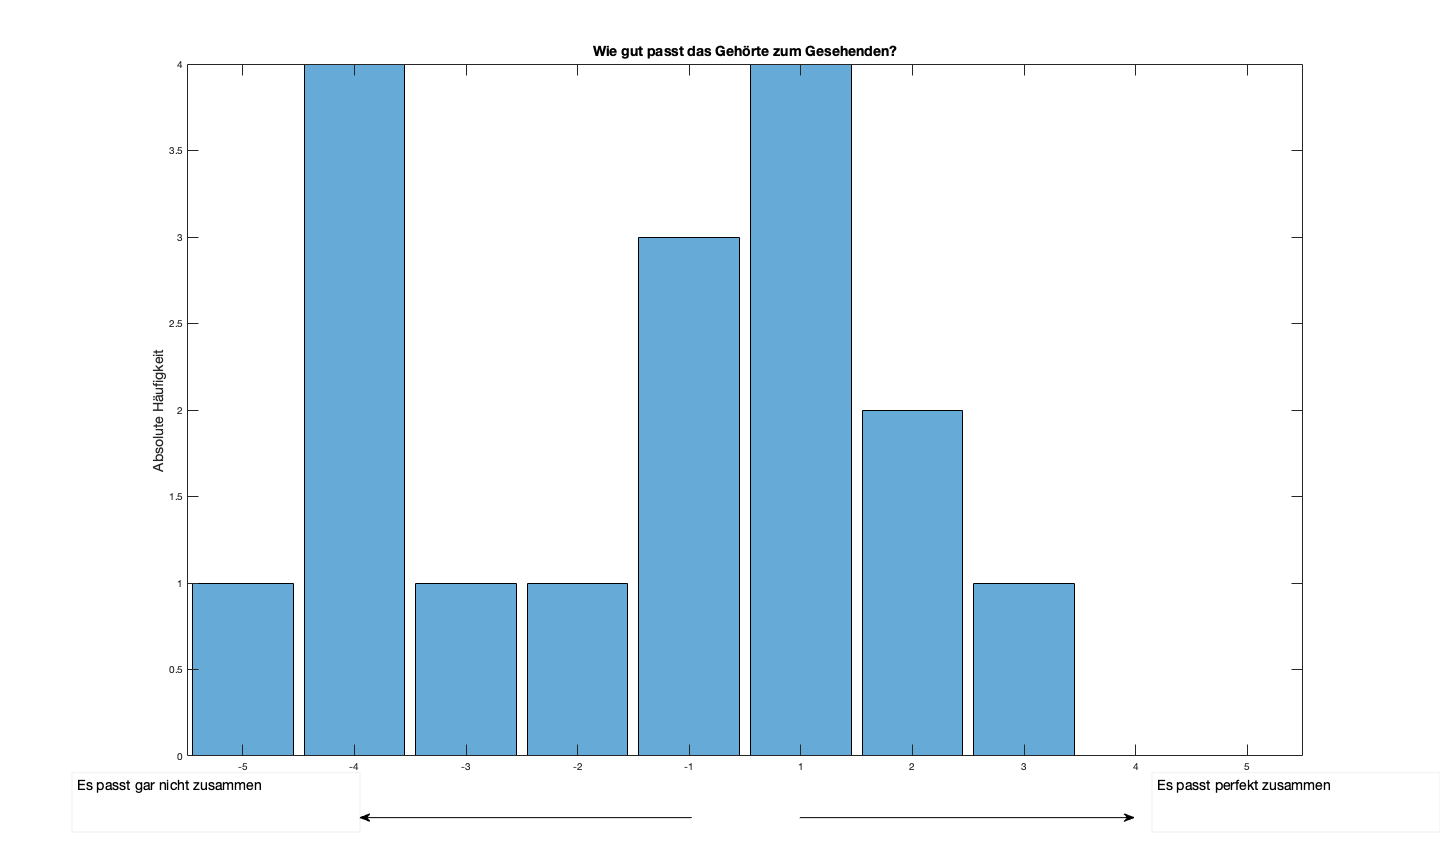
\includegraphics[width = 18cm, height = 10cm]{Szene_1_Frage_1.png}
\caption{Histogramm: Wie gut passen Visuelles und Auditives in Szene 1 zusammen?}
\label{fig:Szene_1_Frage1}
\end{figure} 

Bei der Beurteilung, ob Visuelles und Auditives zusammen passen waren die Meinungen sehr unterschiedlich, siehe Abbildung \ref{fig:Szene_1_Frage1}. Wohingegen sieben Probanden die visuelle und auditive  Darbietung als wenig bis gar nicht als zusammenpassend empfunden haben, haben nur für drei Probanden diese halbwegs zusammengepasst. Damit kann für die erste Szene festgehalten werden, dass die auditive und visuelle Darbietung eher geringfügig zusammen passen. \\

Grund für die eher suboptimale Darbietung könnte unter anderem sein, dass die virtuelle Schallquelle nicht auf dem Adler sondern im Adlernest liegt und daher das gehörte Geräusch nicht zur Position des Adlers passt. Allerdings könnte das Geräusch auch an sich als unpassend zum 3D-Modell des Adlers bewertet werden. Des Weiteren muss immer beachtet werden, dass das Visuelle statisch ist, während das Auditive sich zeitlich verändert. \\ 

Anhand der Abbildung \ref{fig:Szene_1_Frage2} lässt sich deuten, dass das Geräusch wirklich als Bestandteil des Raumes wahrgenommen wird. Für nur zwei Probanden wirkt das Geräusche als halbwegs unrealistisch, während es für alle anderen Probanden als halbwegs realistische bis komplett realistische Quelle im Raum wahrgenommen wird. Es kann für die erste Szene daher von einer erfolgreichen Auralisierung gesprochen werden, bei der die Schallquelle wirklich als plausibler Bestandteil des Raumes wahrgenommen werden kann. 

   \begin{figure}[H]
\centering
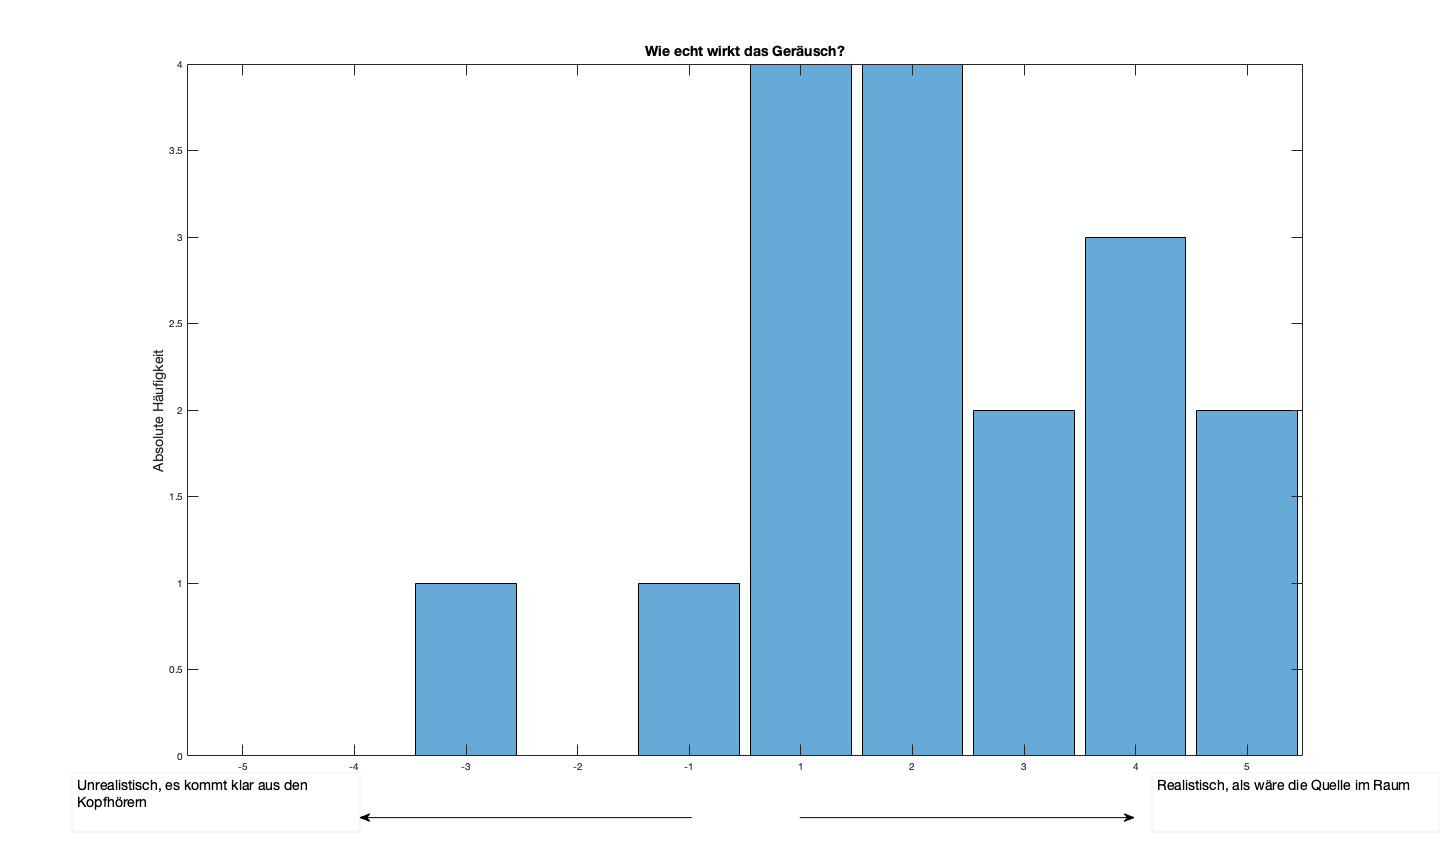
\includegraphics[width = 18cm, height = 10cm]{Szene_1_Frage_2.png}
\caption{Histogramm: Wie echt wirkt das Geräusch im Raum in Szene 1?}
\label{fig:Szene_1_Frage2}
\end{figure} 

Abbildung \ref{fig:Szene_1_Frage3} zeigt eindeutig, dass die Darbietung von fast allen Probanden als unheimlich empfunden wird. 14 der 16 Probanden haben dabei die Darbietung mit drei oder höher auf der \glqq Unheimlichkeits\grqq{}-Skala bewertet. Die Darbietung scheint, wie es die Bewertungen erkennen lassen, wirklich unheimlich bei den Probanden angekommen zu sein.\\

Vereint man diese Erkenntnis mit den Ergebnisse aus Abbildung \ref{fig:Szene_1_Frage2}, dann bekräftigt das empfundene Unbehagen der Probanden die These eines \glqq Uncanny-Valley\grqq{}-Effekts für realistisches, räumliches Audio. Die Schallquelle wird größtenteils als realistische Quelle im Raum wahrgenommen und gleichzeitig wird bei fast allen Probanden durch die Darbietung Unbehagen ausgelöst. Dieser Aspekt soll auch in den folgenden Szene noch weiter beobachtet werden. \\

Anhand der Ergebnisse der Fragen lässt sich schwer eine Aussage über das Immersionsempfinden der Probanden aufstellen. Die weitläufige Verteilung der Antworten auf die Frage, ob Visuelles und Auditives als zusammenpassend wahrgenommen werden lässt vermuten, dass die Probanden auch unterschiedliche stark in die virtuelle Welt eintauchen konnten. Besonders die Tatsache, dass die Szene fast ausnahmslos als unheimlich empfunden worden ist, könnte, trotz der empfundenen Echtheit der Schallquelle im Raum, eine Immersion der Probanden in die erweiterte Realität verhindert haben. \\


   \begin{figure}[H]
\centering
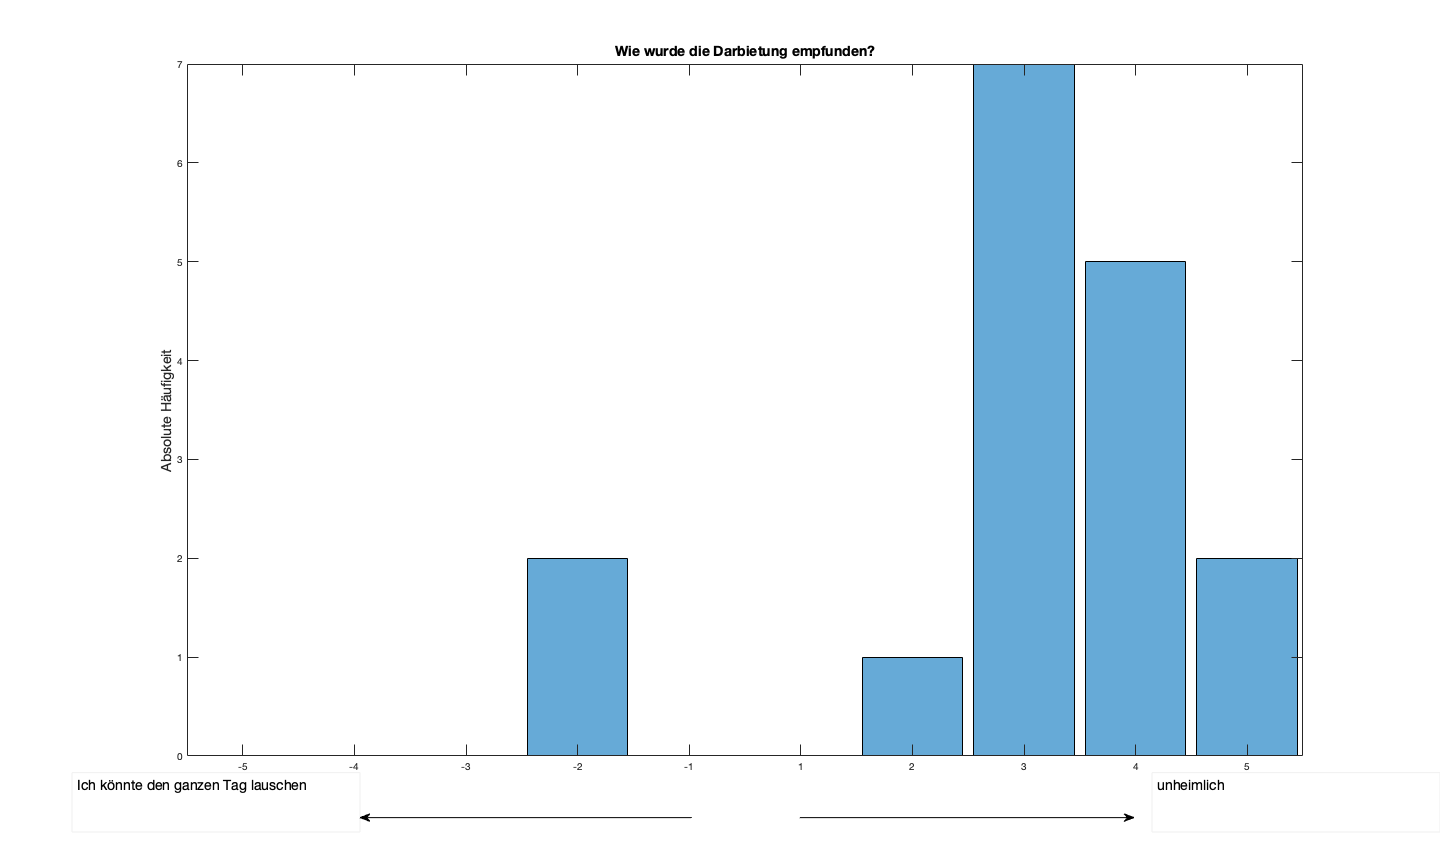
\includegraphics[width = 18cm, height = 10cm]{Szene_1_Frage_3.png}
\caption{Histogramm: Wie angenehm war die Darbietung von Szene 1?}
\label{fig:Szene_1_Frage3}
\end{figure} 



 \subsection{Szene 2: Wolfsheulen}
 Bei der zweiten Szene wurden die selben Audio-Einstellungen wie bei der ersten Szene gewählt. Die virtuelle Schallquelle wurde hierbei auf dem schwarzen Wolf im Wald platziert und gibt das Heulen eines Wolfes wieder. Das Besondere an der Szene ist, dass neben dem schwarzen Wolf ein weiterer, offensichtlicherer, weißer Wolf zu sehen ist, der als potentielle virtuelle Schallquelle dienen könnte. \\
 
In Abbildung \ref{fig:Szene_2_data} lässt sich erkennen, dass ein Großteil der Probanden die virtuelle Schallquelle auf dem weißen Wolf lokalisiert hat und nur wenige an der Position des schwarzen Wolfes. Einige wenige haben die virtuelle Schallquelle außerhalb des Waldes aber in der richtigen Höhe wahrgenommen und zwei Probanden haben die Hörereignisse wieder unmittelbar über dem Gebirge lokalisiert.  \\

Anscheinend konnte durch die räumliche Wiedergabe nicht darauf geschlossen werden, welcher der Wölfe die virtuelle Schallquelle darstellt. Da der weiße Wolf, etwas größer und von nicht so vielen Bäumen verdeckt worden ist, wurde das Hörereignis vermutlich eher in seiner Richtung lokalisiert. Es gilt also aufzupassen, dass beim Einsatz von räumlichem Audio nicht zu viele visuelle, potentielle Schallquellen im Raum sind, da es sonst zu Fehlinterpretationen bezüglich des Nutzers kommen kann. 
 
   \begin{figure}[H]
\centering
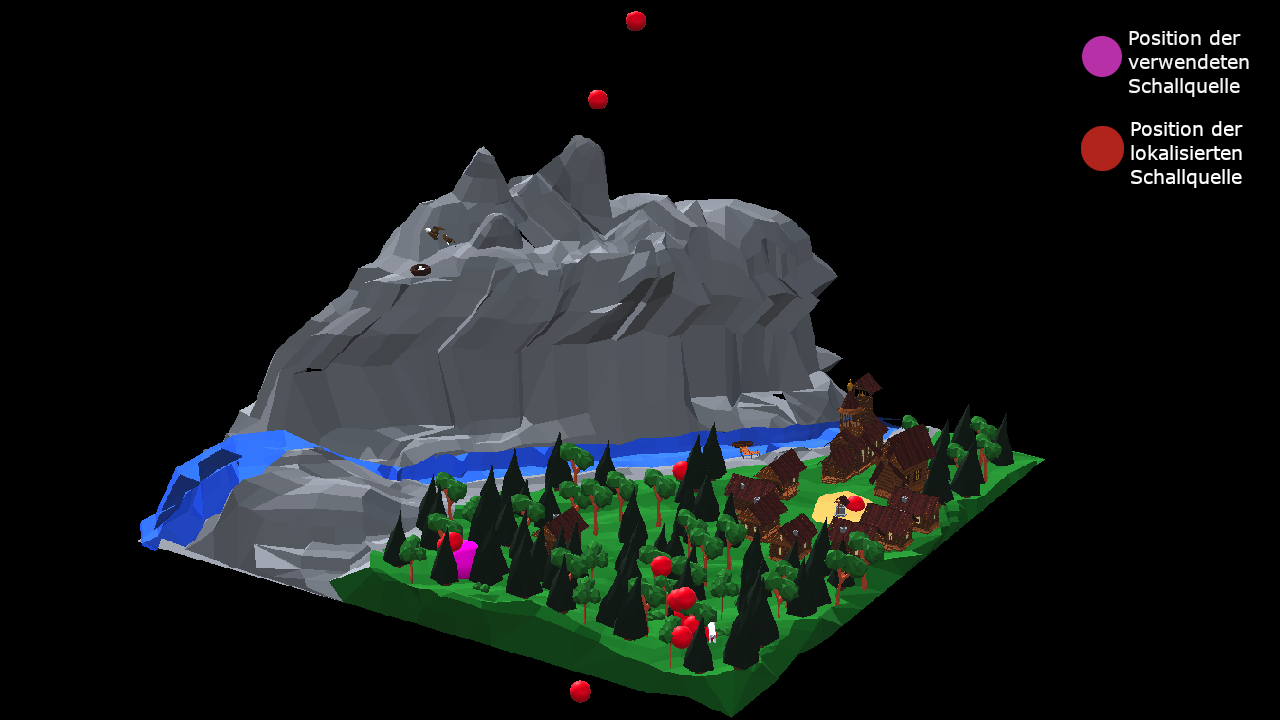
\includegraphics[width = 16cm, height = 9cm]{Szene_2_data.png}
\caption{Visualisierung der lokalisierten Schallquellen für Szene 2}
\label{fig:Szene_2_data}
\end{figure} 

Wie auch schon in der ersten Szene ist das Empfinden, ob das Visuelle und das Auditive zusammenpassen wieder sehr unterschiedlich, jedoch im Vergleich zur ersten Szene etwas positiver, siehe Abbildung \ref{fig:Szene_2_Frage1}. Während die meisten Probanden das Zusammenspiel wieder als mittelmäßig bewertet haben, so gibt es diesmal weniger die behaupten, dass das Gehörte und das Gesehene gar nicht zusammen passen würden. 

   \begin{figure}[H]
\centering
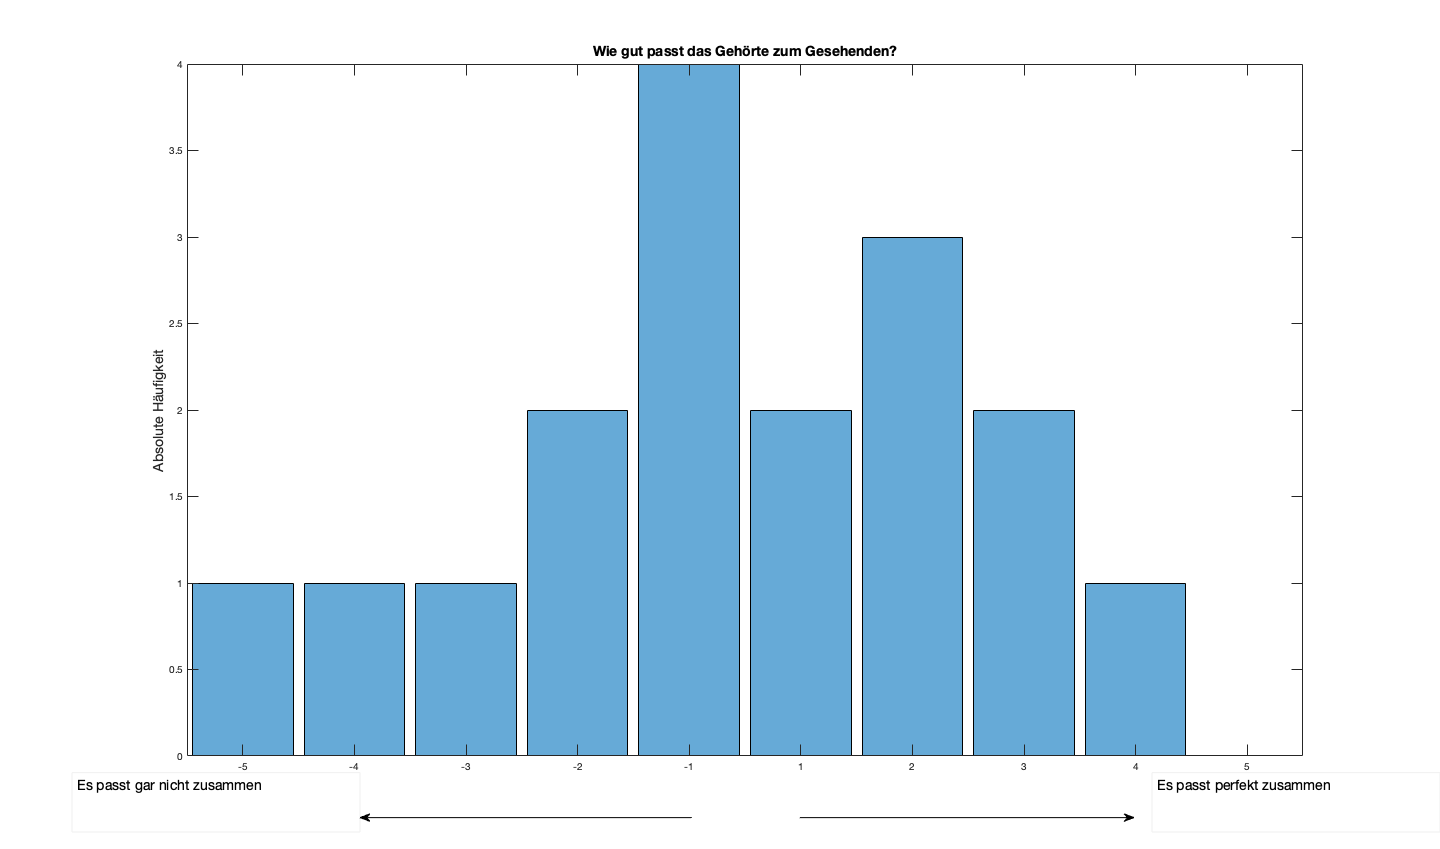
\includegraphics[width = 18cm, height = 10cm]{Szene_2_Frage_1.png}
\caption{Histogramm: Wie gut passen Visuelles und Auditives in Szene 2 zusammen ?}
\label{fig:Szene_2_Frage1}
\end{figure} 

Anhand Abbildung \ref{fig:Szene_2_Frage2} lässt sich erkennen, dass das Geräusch als noch realer eingestuft worden ist als der Adlerschrei in Szene 1. Hierfür könnte es mehrere Gründe geben. Zum einen befindet sich die virtuelle Schallquelle in einer anderen Höhe als die der ersten Szene, so dass andere kopfbezogene Übertragungsfunktionen verwendet werden, die unter Umständen weniger gut zutreffend für die Probanden sind. Zum anderen könnte auch das Geräusch selbst ausschlaggebend sein.\\

Inhaltlich ist das Heulen eines Hundes bzw. Wolfes in einem Raum ein vertrauteres Geräusch als der Schrei eines Vogels, der vermutlich so niemals in einem Laborraum, auf der Höhe eines Tisches vorkommen wird. Die inhaltliche Einordnung des Geräusches könnte bewirken, dass das Heulen eines Hundes eher als plausibles Hörereignis im Raum wahrgenommen wird als der Schrei eines Adlers.  

   \begin{figure}[H]
\centering
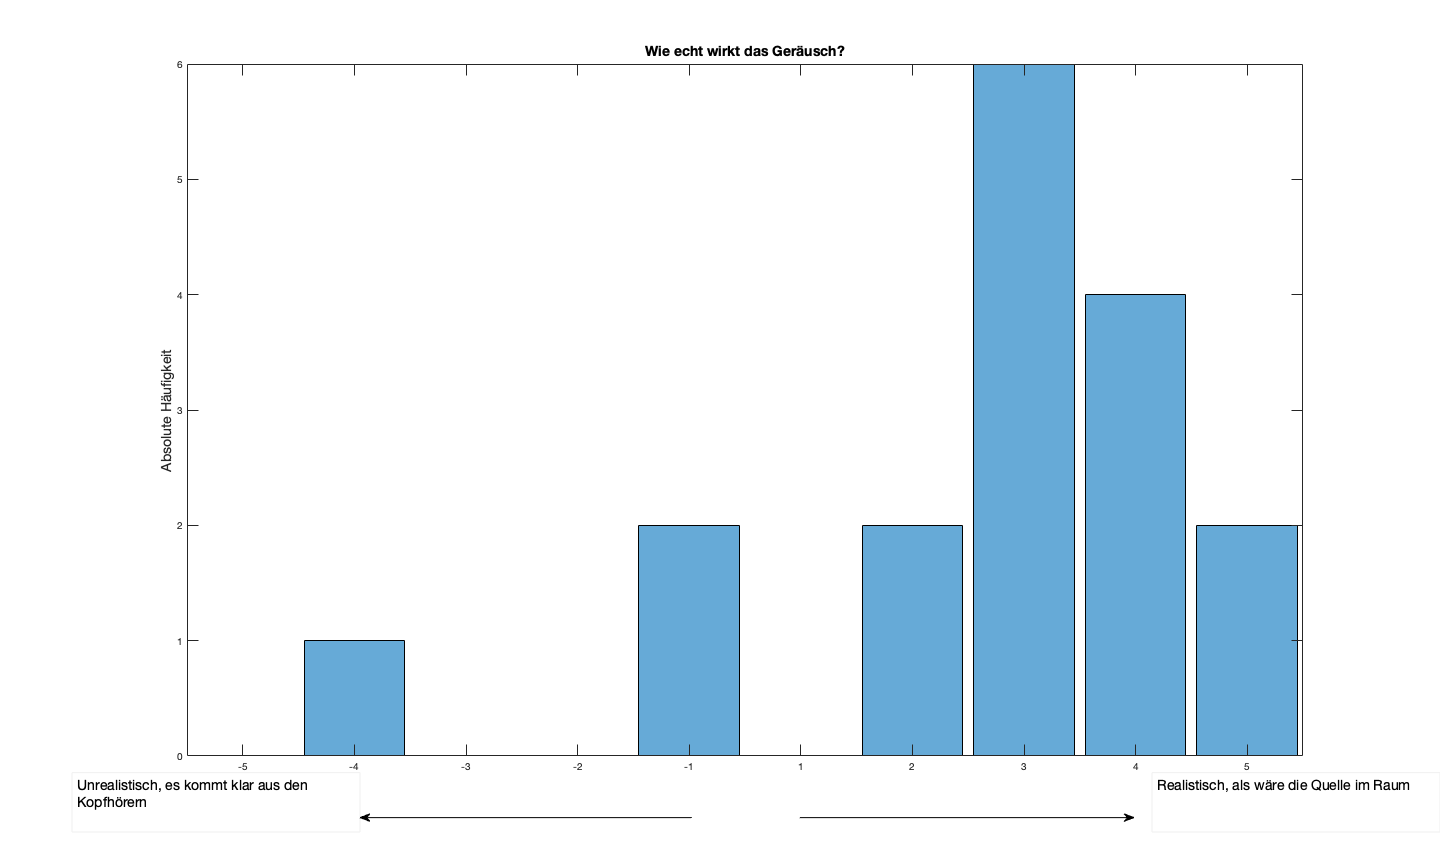
\includegraphics[width = 18cm, height = 10cm]{Szene_2_Frage_2.png}
\caption{Histogramm: Wie echt wirkt das Geräusch im Raum in Szene 2?}
\label{fig:Szene_2_Frage2}
\end{figure} 

In Abbildung \ref{fig:Szene_2_Frage3} lässt sich erkennen, dass die Darbietung von Szene 2 genau wie die erste Szene auf die meisten Probanden sehr unheimlich gewirkt hat, es jedoch auch mehr Ausnahmen gab als bei Szene 1. Ein Proband hat hierbei die Szene sogar mit der angenehmsten Bewertungsstufe versehen. Drei weitere Probanden haben die Szene ebenfalls als angenehm eingestuft. Das allgemeine Unwohlsein bei der Szene könnte wie bei der vorherigen Szene  durch den zu hohe Realismus der Audio-Wiedergabe impliziert werden. \\ 

Ein anderer für das Unwohlsein der Probanden bei der Szene könnte auch der inhaltliche Kontext des Geräusches sein. Dem Heulen eines Wolfes könnte mit Angst gegenübergetreten werden und dem Heulen eines Hundes mit Empathie. In beiden Fällen bedeutet dies, dass die Szene Unbehagen auslöst.  \\

Wie schon bei der ersten Szene lässt sich anhand der Probandenergebnisse nicht wirklich beurteilen, wie gut eine Immersion der Probanden in die erweiterte Realität gelungen ist. Das empfundene Unbehagen der Probanden lässt auch in dieser Szene vermutlich keine Immersion zu. 

   \begin{figure}[H]
\centering
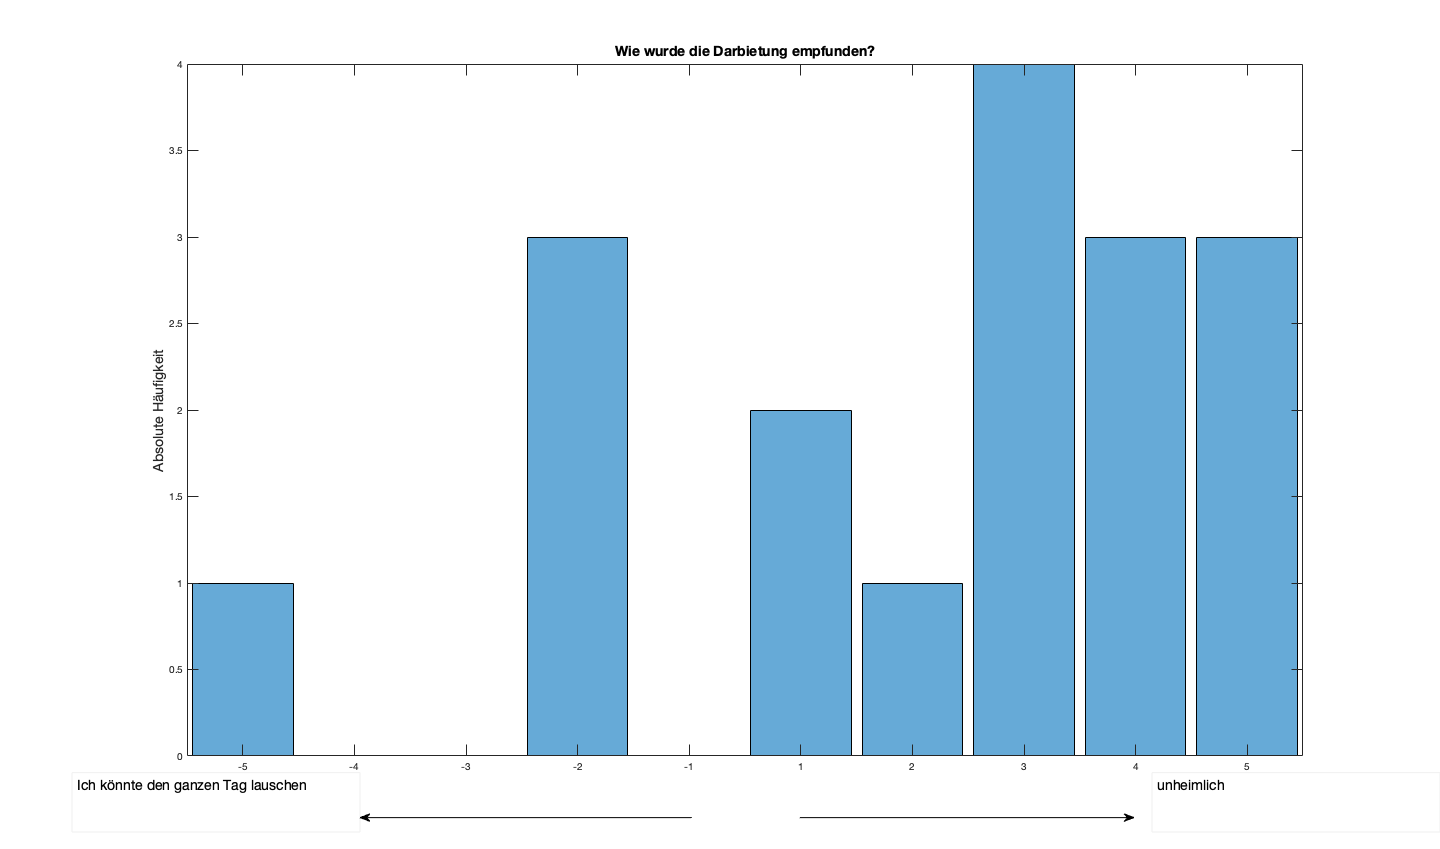
\includegraphics[width = 18cm, height = 10cm]{Szene_2_Frage_3.png}
\caption{Histogramm: Wie angenehm war die Darbietung von Szene 2?}
\label{fig:Szene_2_Frage3}
\end{figure} 

 \subsection{Szene 3: Kirchenglocken}
Im Vergleich zu den ersten beiden Szenen wird in Szene 3 keine Form von räumlichen Audio verwendet. Stattdessen werden das Erklingen von Kirchenglocken mono über die Kopfhörer wiedergegeben.\\

Wie anhand von Abbildung \ref{fig:Szene_3_data} zu sehen ist, lokalisieren die meisten Probanden das Hörereignis im vorderen Kirchturm. Daraus lässt sich schließen, dass auch ohne räumliches Audio die Schallquellen fast ausschließlich dort lokalisiert werden, wo es vom inhaltlichen Kontext her hin passt.\\

Auffällig sind hierbei die wenigen Ausreißer, die fast alle auf einer Vertikalen in der Mitte der virtuellen Welt liegen und dabei alle eine unterschiedliche Höhe haben. Dies liegt vermutlich daran, dass durch die Mono-Wiedergabe keine interauralen Laufzeitunterschiede zustande kommen und dies sonst nur der Fall ist wenn das zu lokalisierende Hörereignis in der Medianebene des Hörerenden liegt. Startet die Szene schaut der Proband zu aller erst gerade auf die Welt, so dass er denken könnte in dieser Ebene müsse die Schallquelle liegen.

 
   \begin{figure}[H]
\centering
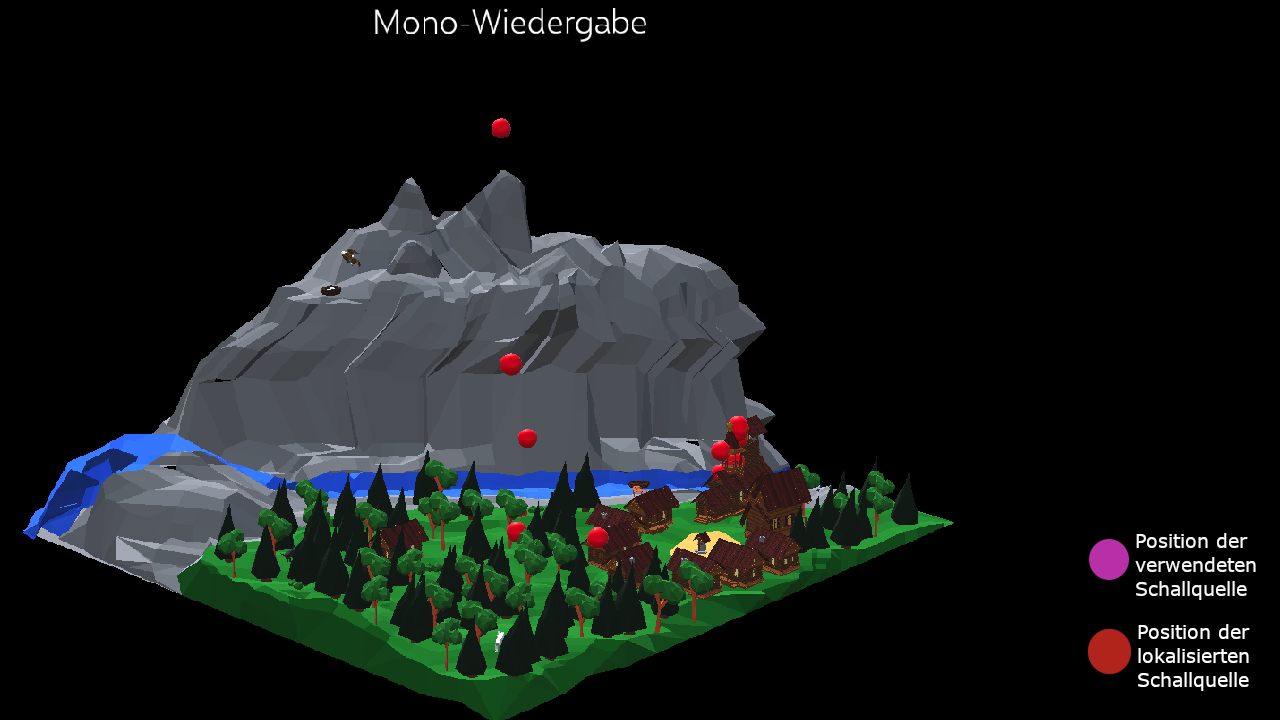
\includegraphics[width = 16cm, height = 9cm]{Szene_3_data.png}
\caption{Visualisierung der lokalisierten Schallquellen für Szene 3}
\label{fig:Szene_3_data}
\end{figure} 

Auch bei der Mono-Wiedergabe werden das Visuelle und  das Auditive als nicht zusammenpassend bewertet. Die Probanden sind sich bis auf einen einzigen einig, dass die Mono-Wiedergabe der Kirchenglocken gar nicht bis kaum zu den virtuellen Kirchenglocken passt.

   \begin{figure}[H]
\centering
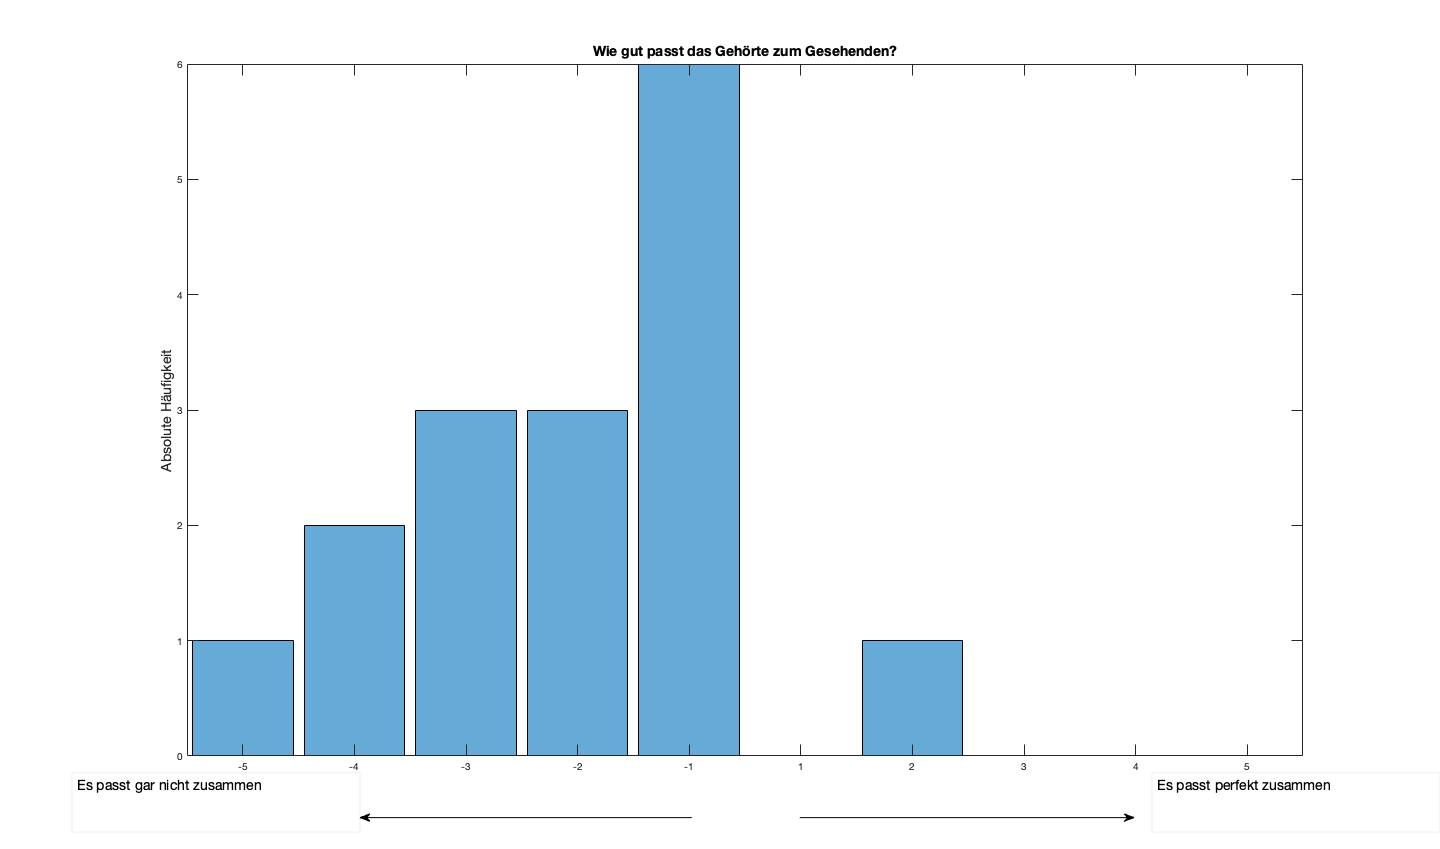
\includegraphics[width = 18cm, height = 10cm]{Szene_3_Frage_1.png}
\caption{Wie gut passen Visuelles und Auditives in Szene 3 zusammen?}
\label{fig:Szene_3_Frage1}
\end{figure} 

Überraschend ist, dass trotz der Mono-Wiedergabe ein Großteil der Probanden das Hörereignis als realistisches Geräusch im Raum wahrgenommen hat, siehe Abbildung \ref{fig:Szene_3_Frage2}. Viele weitere Probanden haben das Geräusch als Teilweise unrealistisch wahrgenommen und nur wenige haben für sich entschieden, dass das Geräusch ganz offensichtlich aus den Kopfhörern kommt. Fraglich ist ob die Probanden, die die Szene als realistisch empfunden haben, den Unterschied zu den ersten Szenen nicht gehört haben oder ob sie den wahrgenommenen Unterschied als irrelevant für die Bewertung der Echtheit ansehen. 

   \begin{figure}[H]
\centering
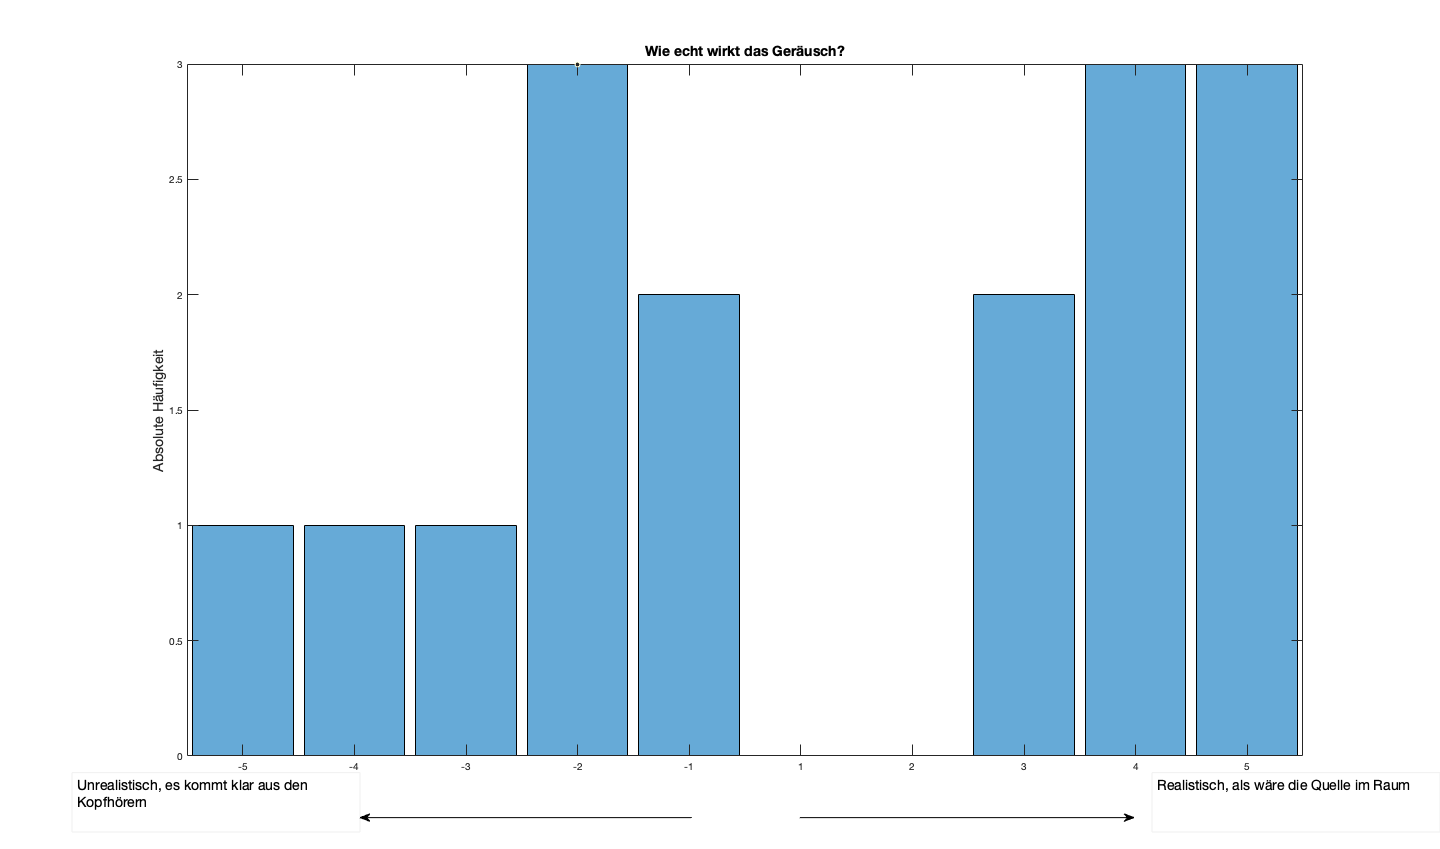
\includegraphics[width = 18cm, height = 10cm]{Szene_3_Frage_2.png}
\caption{Histogramm: Wie echt wirkt das Geräusch im Raum in Szene 3?}
\label{fig:Szene_3_Frage2}
\end{figure} 

In Abbildung \ref{fig:Szene_3_Frage3} lässt sich erkennen, dass wie bei den ersten beiden Szenen viele Probanden die Darbietung als unheimlich empfinden. Der Anteil an Probanden, die die Szene jedoch als angenehm empfinden ist beachtlich höher als bei den ersten beiden Szenen. So empfinden sechs Probanden die Szene eher angenehm als unheimlich. \\

Ein Grund für das angenehmere Darbietungsempfinden könnte sein, dass das das Erklingen von Glocken generell angenehmer ist als das Heulen eines Wolfes oder der Schrei eines Adlers. Dies lässt sich unter anderem auch am bereits erwähnten harmonischen Klang des Geräusches  begründen.  \\

Natürlich könnte das im Vergleich zu den Szenen mit räumlichem Audio angenehmere Darbietungsempfinden auch das Resultat der fehlenden, räumlichen Anpassung der Audio-Signale sein, dessen extremer Realismus beim Hörenden Unbehagen bewirken könnte.

Mit fünf Probanden, die die Szene als komplett unheimlich bewerten und den Ergebnissen aus den vorherigen Szenen liegt es nah, dass die generelle Darbietung unabhängig vom Geräusch als unheimlich wahrgenommen werden könnte. Das Unwohlsein könnte dementsprechend auch einfach durch die ungewohnte Situation mit der HoloLens in einer Mixed-Reality-Umgebung evoziert werden. \\


   \begin{figure}[H]
\centering
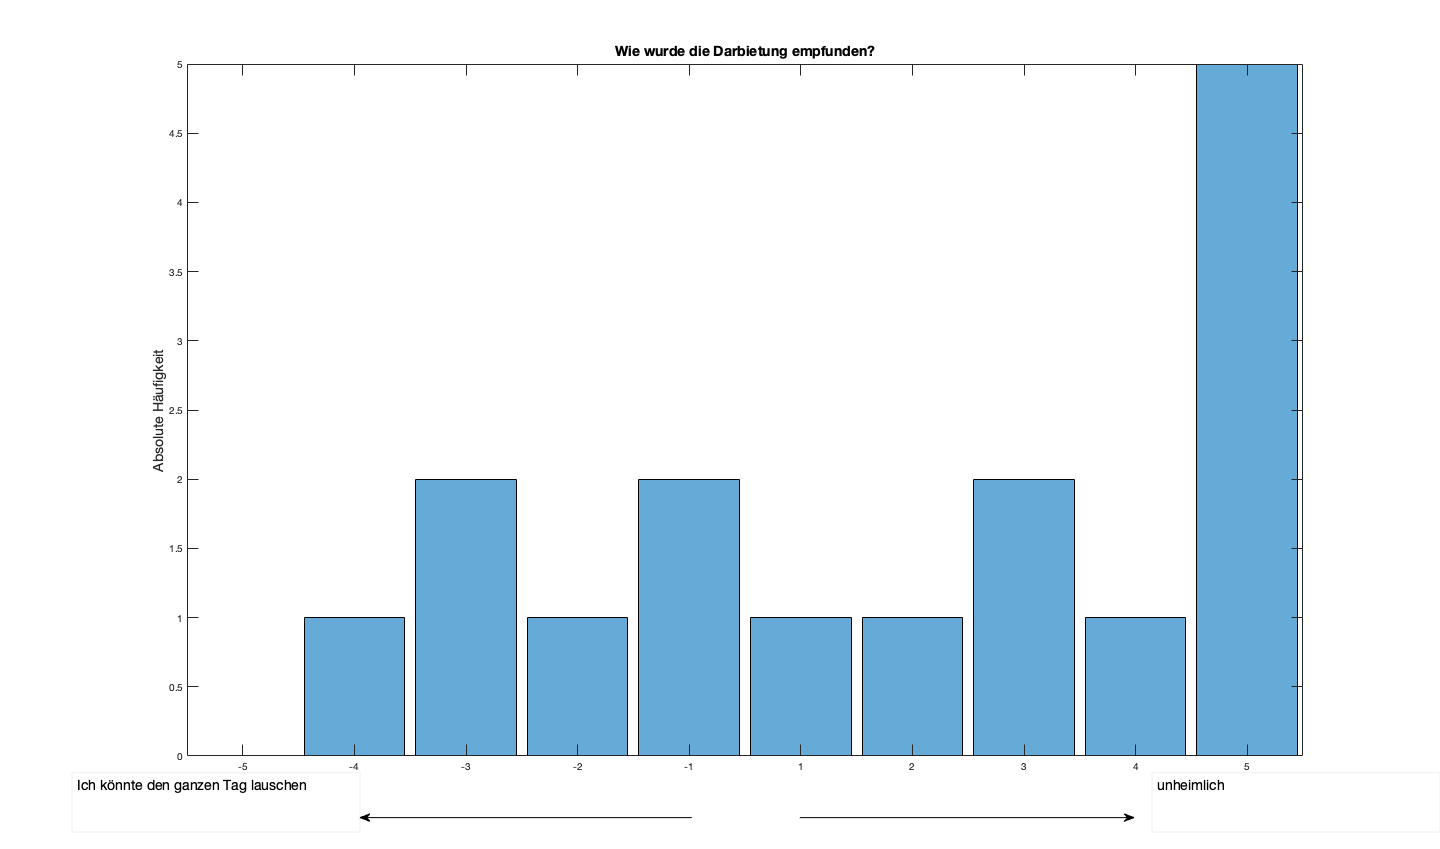
\includegraphics[width = 18cm, height = 10cm]{Szene_3_Frage_3.png}
\caption{Histogramm: Wie angenehm war die Darbietung von Szene 3?}
\label{fig:Szene_3_Frage3}
\end{figure} 

Auch in der dritten Szene ist zu vermuten, dass die meisten Probanden, wie in dieser Szene zu erwarten war,  keine wirkliche Immersion empfinden konnten. Grund dafür ist, dass die visuellen und auditiven Reize erneut als nicht zusammenpassend empfunden worden sind, die Hörereignisse zudem eher als aus dem Kopfhörer kommend wahrgenommen worden sind und auch hier die Darbietung bei den meisten eher Unbehagen ausgelöst hat. 

 \subsection{Szene 4: Adler in der Luft}
In der vierten Szene werden wieder die Standart-Einstellungen für das räumliche Audio des Hörversuchs übernommen. Die virtuelle Schallquelle wurde hierbei über den Probanden platziert, so dass diese um den visualisierten Adler sehen zu können, nach oben schauen mussten. Bei dem Geräusch handelt es sich erneut um den Adlerschrei aus der ersten Szene. Im Vergleich zur ersten Szene sollte die Position des Geräusches nun besser an den inhaltlichen Kontext angepasst sein. \\

Abbildung \ref{fig:Szene_4_data} zeigt, erneut die Verteilung der lokalisierten Schallquellen. Es ist zu erkennen, dass wie bisher in keiner anderen Szene vorher die virtuelle Schallquelle im Raum gestreut lokalisiert worden ist. Während zwei Probanden den Adler über sich ausmachen und als Schallquelle identifizieren konnten, haben vier andere Probanden erneut das Hörereignis beim Adler unmittelbar über dem Berg lokalisiert. \\

Bemerkenswert ist, dass die meisten Probanden erkennen konnten, dass das Hörereignis aus nicht mehr aus der Richtung der tiefer fliegenden Adler kommt und stattdessen die Schallquelle irgendwo im Raum lokalisiert haben. Dabei variieren zum ersten mal für die Szenen mit räumlichem Audio die Höhen der platzierten roten Kugeln. Die Probanden konnten also feststellen, dass die virtuelle Schallquelle über der Welt liegen muss, hatten aber Probleme ohne offensichtliche Visualisierung die richtige Position und die richtige Höhe zu ermitteln. Es ist anzunehmen, dass die meisten Probanden den Adler nicht mal sehen konnten, weil sie soweit oben keine Visualisierung mehr erwartet hätten. Der Einsatz von räumlichem Audio alleine reicht also nicht aus um den Fokus auf Objekte außerhalb des natürlichen Sichtfeldes zu legen. 

   \begin{figure}[H]
\centering
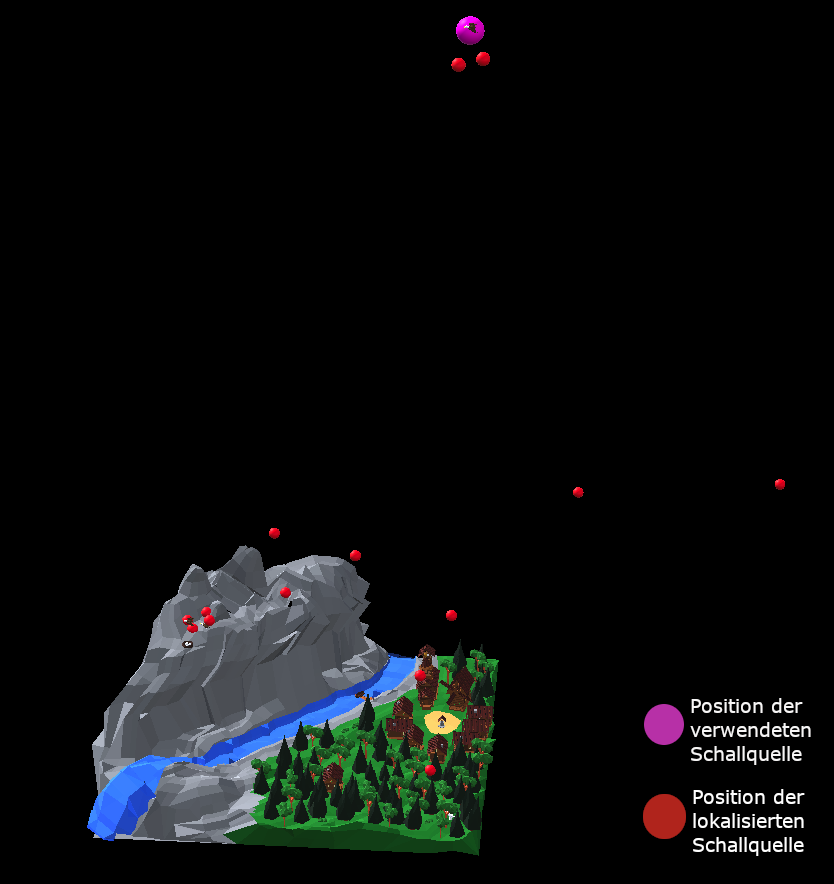
\includegraphics[width = 13cm, height = 14 cm]{Szene_4_data_2.png}
\caption{Visualisierung der lokalisierten Schallquellen für Szene 4}
\label{fig:Szene_4_data}
\end{figure} 

In Abbildung \ref{fig:Szene_4_Frage1} lässt sich erkennen, dass im Vergleich zur ersten Szene mit dem selben Geräusch das Empfinden, ob Visuelles und Auditives zusammenpassen, tatsächlich etwas positiver ausfällt. Während in der ersten Szene noch für sechs Probanden das Gehörte und das Gesehene sehr wenig bis gar nicht zusammengepasst haben, so gibt es bei der vierten Szene  nur noch 3 Probanden die das Zusammenspiel so negativ bewertet haben. Der Zahl der Probanden, die bei der Frage keiner der Antworten wirklich zustimmen konnten ist hierbei dementsprechend etwas gestiegen, während der Anteil der Probanden für die die Reize zusammen passten gleich geblieben ist.\\ 

Es gilt bei der Beobachtung der Ergebnisse dieser Umfrage zu beachten, dass vermutlich die wenigsten den Adler über sich wirklich gesehen haben. Das leicht verbesserte Empfinden für das Zusammenspiel des Auditiven mit dem Visuellen könnte daher unterschiedliche Gründe haben. Einer der Gründe könnte sein, dass dadurch das der Adlerschrei nun aus der Luft kommt die allgemeine Plausibilität der Szene gestiegen ist, da der inhaltliche Kontext besser zum Gesehenen passt. Ein weiterer Grund könnte sein, dass der Proband sich generell an das Tragen der HoloLens und den Anblick der Welt gewöhnt hat und daher das Visuelle anders wahrnimmt. 


   \begin{figure}[H]
\centering
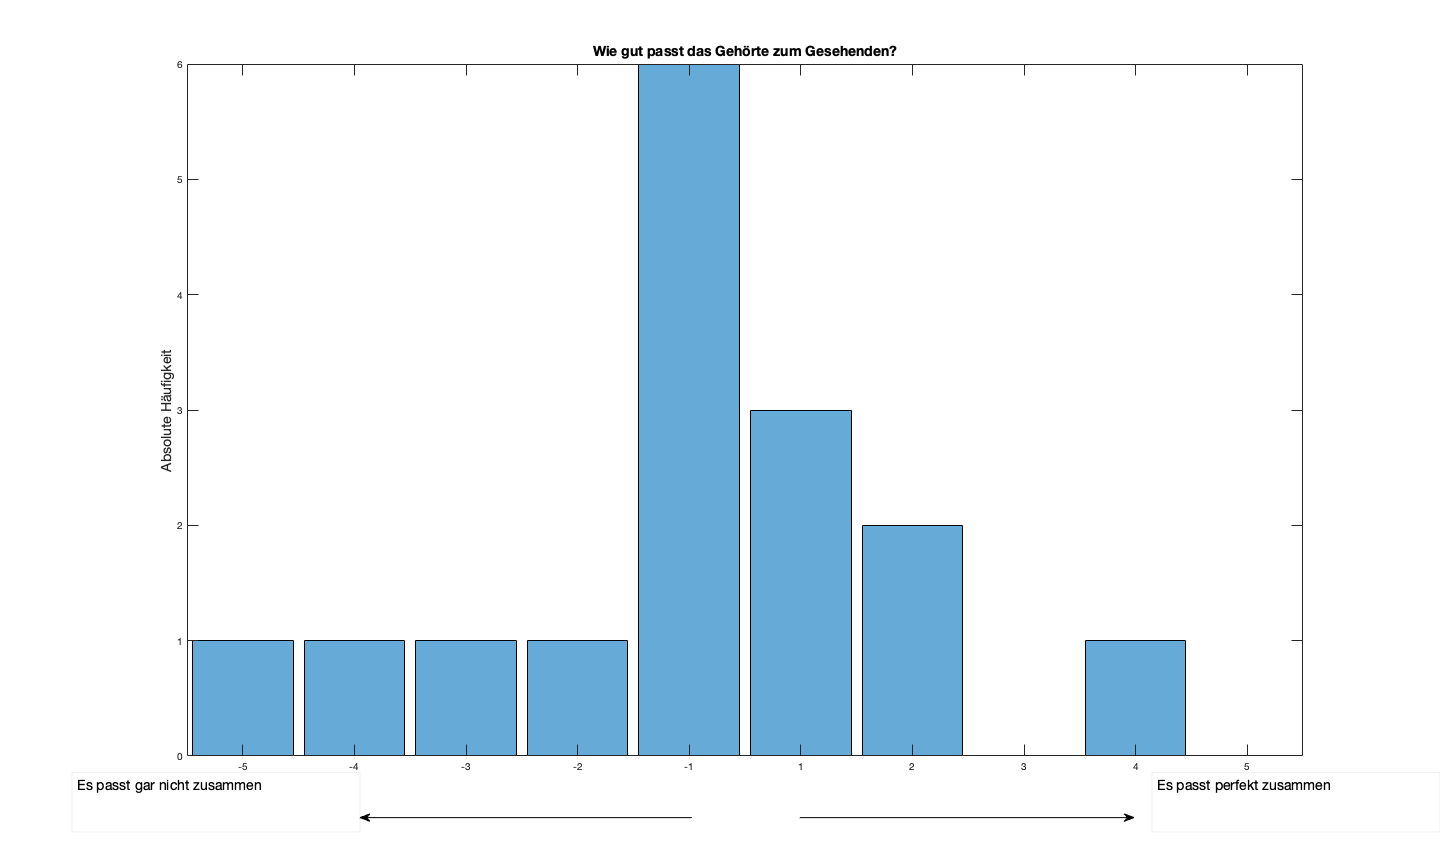
\includegraphics[width = 18cm, height = 10cm]{Szene_4_Frage_1.png}
\caption{Histogramm: Wie gut passen Visuelles und Auditives in Szene 4 zusammen ?}
\label{fig:Szene_4_Frage1}
\end{figure} 

Anhand Abbildung \ref{fig:Szene_4_Frage2} ist zu sehen, dass zehn Probanden das Geräusch als realistische Quelle im Raum beurteilen würden. Damit sind es sogar noch mehr als bei der ersten Szene, die das Geräusch als realistisch beurteilen. Angestiegen ist jedoch auch der Anteil, der Probanden, die das Geräusch als unrealistisch bewerten. \\

Die Ergebnisse könnten damit zu begründen sein, dass die meisten Probanden erkannt haben, dass das Hörereignis nicht mehr unmittelbar in der virtuellen Welt stattfand und es deshalb als plausibler eingestuft worden ist. Gleichzeitig konnten einige, wie es in Abbildung \ref{fig:Szene_4_data} gezeigt wird, nicht erkennen, dass das Geräusch nicht mehr dort ist wo es sich noch in der ersten Szene befand. Geht man davon aus, dass das Geräusch wirklich noch auf den Adlern über dem Berg liegt, dann klingt das Audio-Signal, dass an den Adler über dem Probanden angepasst worden ist natürlich unplausibel und daher unrealistisch. 


   \begin{figure}[H]
\centering
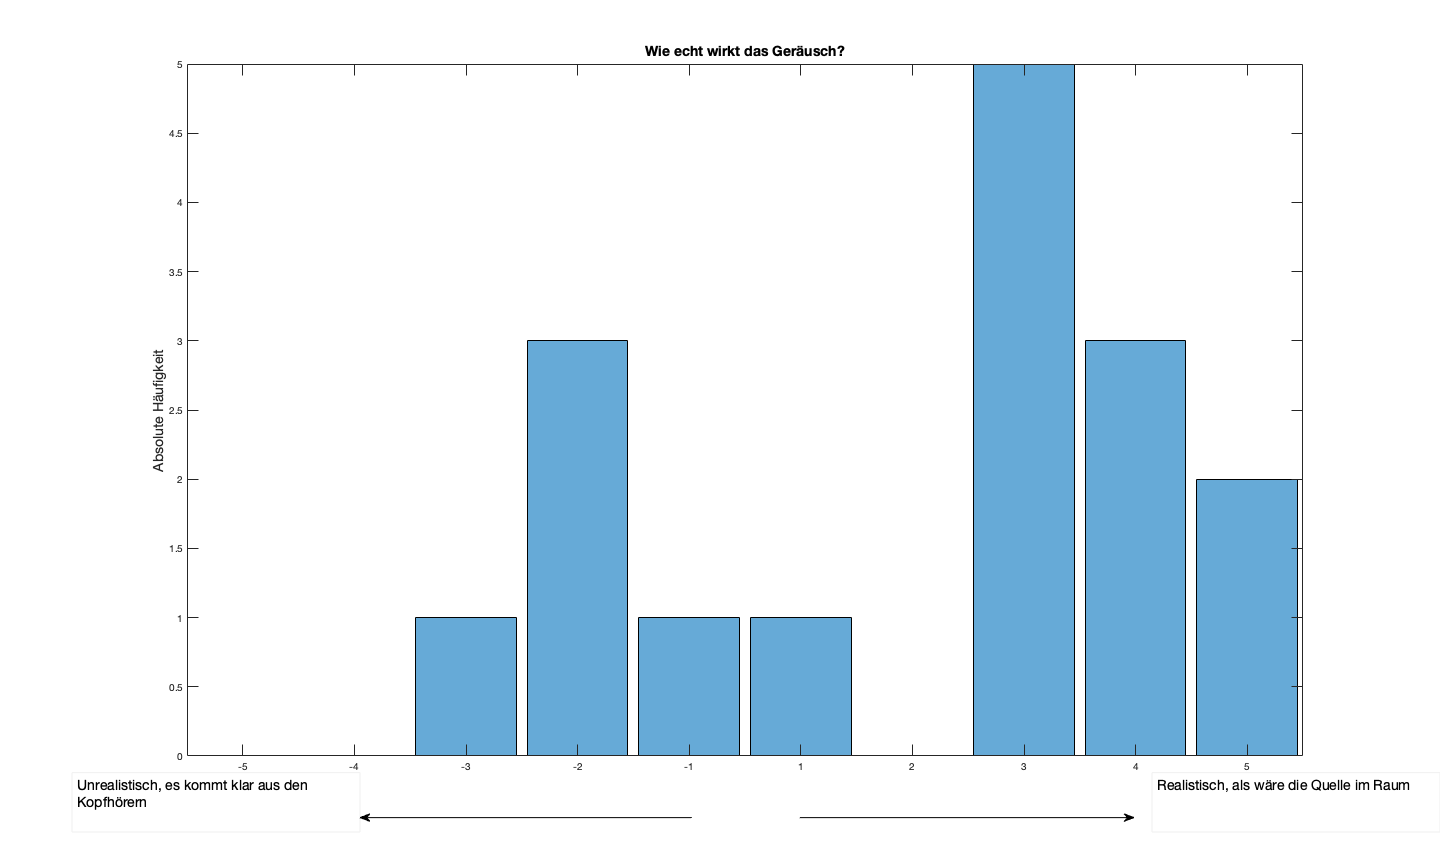
\includegraphics[width = 18cm, height = 10cm]{Szene_4_Frage_2.png}
\caption{Histogramm: Wie echt wirkt das Geräusch im Raum in Szene 4?}
\label{fig:Szene_4_Frage2}
\end{figure} 

Die Darbietung von Szene 4 wurde, wie es in Abbildung \ref{fig:Szene_4_Frage3} gezeigt wird,  von vielen Probanden als deutlich angenehmer empfunden als die Darbietung der ersten beiden Szenen. Während bei der ersten Szene noch ca. 90 \% der Probanden die Darbietung eher als unheimlich empfunden haben, so haben in der vierten Szenen schon mehr als 40 \% die Darbietung als eher angenehm bewertet. Trotz dessen evoziert die Darbietung bei den meisten immer noch ein eher unangenehmes Gefühl.\\ 

Das zunehmend positivere Darbietungsempfinden der Szene könnte damit zusammenhängen, dass wie bereits erwähnt das Geräusch einfach inhaltlich plausibler ist, dadurch dass es von oben kommt. Andererseits könnte die Darbietung auch durch die Gewöhnung an die HoloLens immer angenehmer werden. \\ 

Theoretisch könnte aber auch die Tatsache, dass das Hörereignis nicht mehr in der unmittelbaren Umgebung des Hörenden liegt dafür verantwortlich sein, dass die Darbietung nicht mehr so unheimlich bewertet wird wie bei den anderen Szenen. Möglicherweise tritt der vermute \glqq Uncanny-Valley\grqq{}-Effekt nur dann für realistisches, räumliches Audio auf, wenn sich das Geräusch direkt vor dem Betrachter, bzw. im Sichtfeld, befindet. Da die meisten erkannt haben, dass das Hörereignis nicht direkt in der virtuellen Welt stattgefunden hat, könnte es sein, dass sie sich von diesem Geräusch auch nicht eingeschüchtert oder bedroht gefühlt haben.
 

   \begin{figure}[H]
\centering
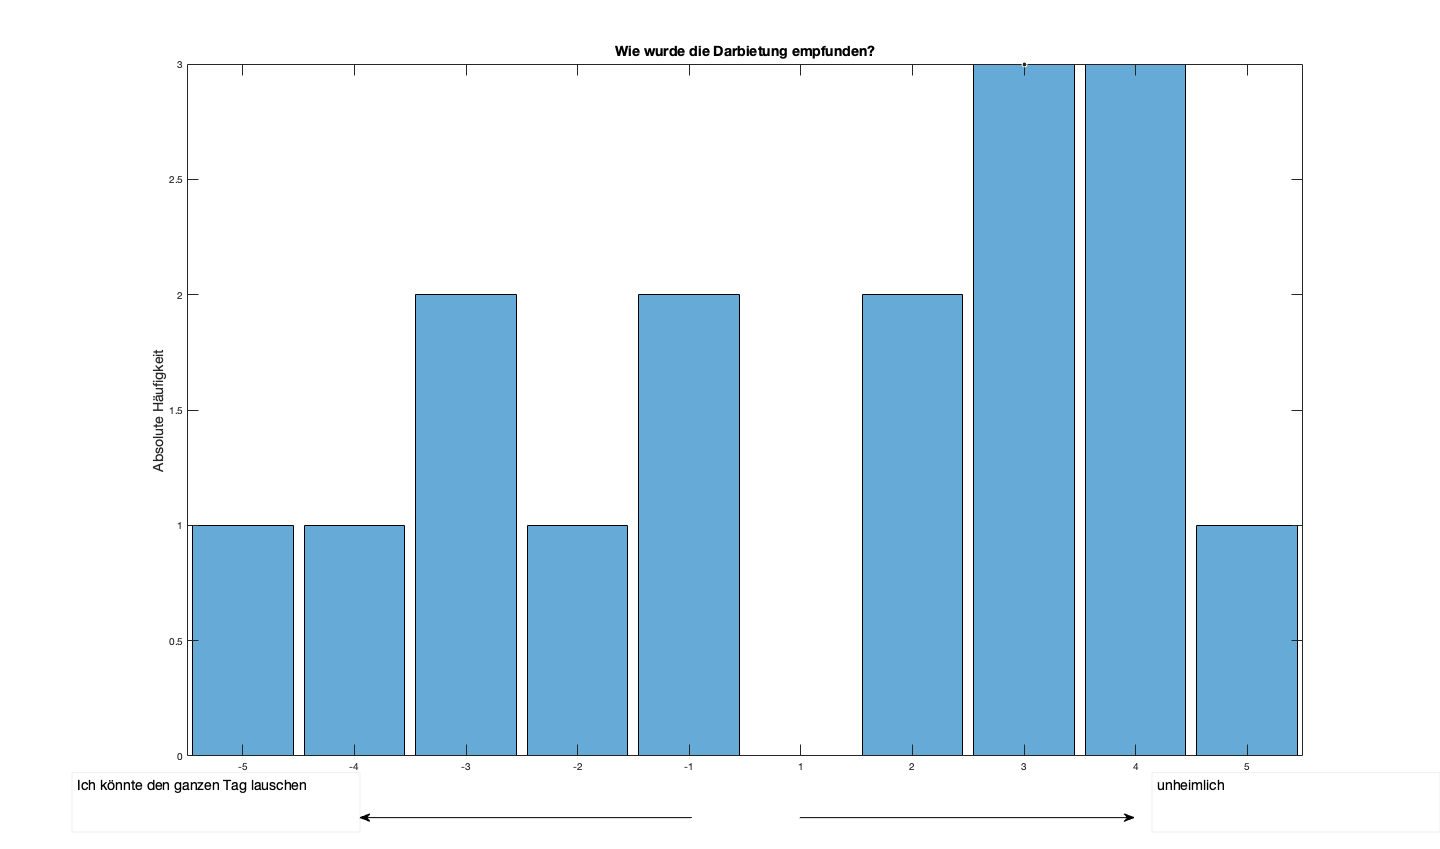
\includegraphics[width = 18cm, height = 10cm]{Szene_4_Frage_3.png}
\caption{Histogramm: Wie angenehm war die Darbietung von Szene 4?}
\label{fig:Szene_4_Frage3}
\end{figure} 



 \subsection{Szene 5: Flussrauschen}
Die letzte Szene des Versuchs enthält im Vergleich zu den anderen Szenen zwei virtuelle Schallquellen. Als Geräusch wird das Rauschen eines Flusses über beide Schallquellen gleichermaßen wiedergegeben. Der Proabnd hat auch hier nur eine Kugel zu platzieren, da erwartet wird, dass sich eine Phantomschallquelle bilden müsste. Auch hier werden die für den Versuch gewählten Standart-Einstellungen verwendet. Die eine Schallquelle befindet sich hierbei an der Quelle des Flusses und die andere den Fluss abwärts im Boot. \\ 

Abbildung \ref{fig:Szene_5_data} zeigt, dass das Hörereignis erneut sehr weit gestreut lokalisiert worden ist. Die meisten Probanden haben dabei das Hörereignis an der Quelle des Flusses wahrgenommen. Dabei ist zu erwähnen, dass die Probanden fast ausschließlich beim Lokalisieren stehengeblieben sind und daher diese virtuelle Schallquelle näher an den Probanden lag als die zweite im Boot. Nach dem Prinzip der ersten Wellenfront ergibt es also Sinn, dass die Probanden das Hörereignis fast ausschließlich bei der näheren virtuellen Schallquelle wahrgenommen haben, da der Schall dieser Quelle zu erst beim Probanden angekommen ist. Des Weiteren ist davon auszugehen, dass der inhaltliche Kontext eine Rolle bei der Platzierung der roten Kugel gespielt haben könnte, da das Flussrauschen in der Natur vor allem in der wilderen Gebirgslandschaft erwartet werden würde.\\

Zwei Probanden haben die rote Kugel genau in der Mitte zwischen den beiden virtuellen Schallquellen platziert. Dies ergibt vor allem dann Sinn, wenn die Probanden sich so bewegt haben, dass die virtuellen Schallquellen beide gleich weit vom Probanden entfernt waren. Denn dann sollte sich das Hörereignis aufgrund der fehlenden interauralen Laufzeitunterschiede genau in der Mitte der beiden virtuellen Schallquellen bilden. Drei weitere Probanden haben das Hörereignis auf einer Vertikalen zur Welt mittig zwischen den virtuelle Schallquellen lokalisiert. Bei diesen hat sich also das Hörereignis also ebenfalls mittig zwischen den virtuellen Schallquellen gebildet, jedoch haben diese Probanden die Höhe des Hörereignisses anders wahrgenommen.\\ 

An diesem Punkt sollte erwähnt werden, dass bei einer ausgereifteren Version des Hörversuchs neben der Position der roten Kugel auch die Position des Probanden, während der Platzierung gespeichert werden sollte. Auf diese Weise könnten bessere Aussagen darüber getroffen werden, wieso der Proband das Hörereignis so lokalisiert hat, wie er es während des Versuchs getan hat. 



   \begin{figure}[H]
\centering
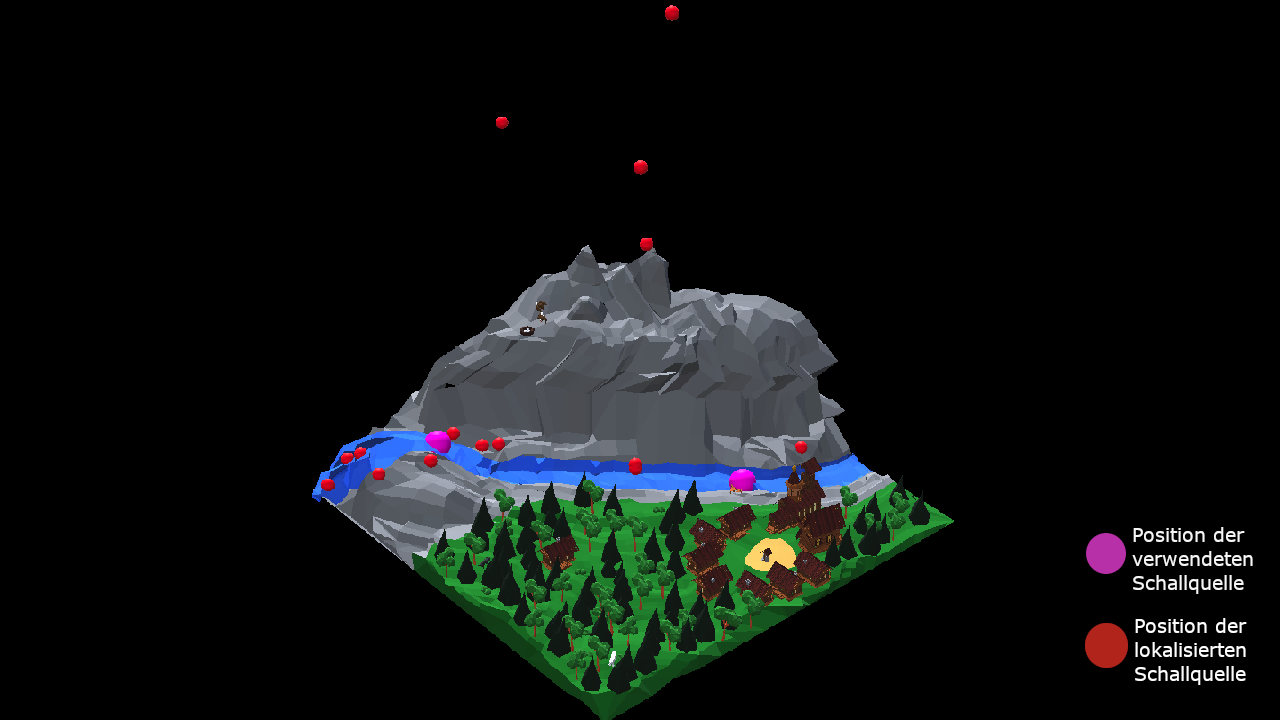
\includegraphics[width = 16cm, height = 9cm]{Szene_5_data.png}
\caption{Visualisierung der lokalisierten Schallquellen für Szene 5}
\label{fig:Szene_5_data}
\end{figure} 

Anhand Abbildung \ref{fig:Szene_5_Frage1} lässt sich feststellen, dass die Probanden sich bei der letzten Szene ziemlich einig sind, dass das Gesehene und das Gehörte nicht sehr gut zusammen passen. Während sieben Probanden keiner der Aussagen komplett zustimmten, so bewertete der Rest der Probanden, dass das Visuelle und das Auditive wenig bis gar nicht zusammen passen. \\

Das Fließen eines Flusses ist ein sehr dynamischer Vorgang, der wie das Flussrauschen vermutlich mit sehr viel Bewegung assoziiert wird. Es ist daher davon auszugehen, dass das statische blaue Wasser in der virtuellen Welt ohne Animation nicht als plausibler visueller Reiz wahrgenommen werden kann. Unter anderem gilt dies auch, deshalb weil sich das Wasser in der virtuellen Welt nicht nach den Gesetzen der Physik verhält und einfach in der Luft schwebt ohne abzufließen. \\

   \begin{figure}[H]
\centering
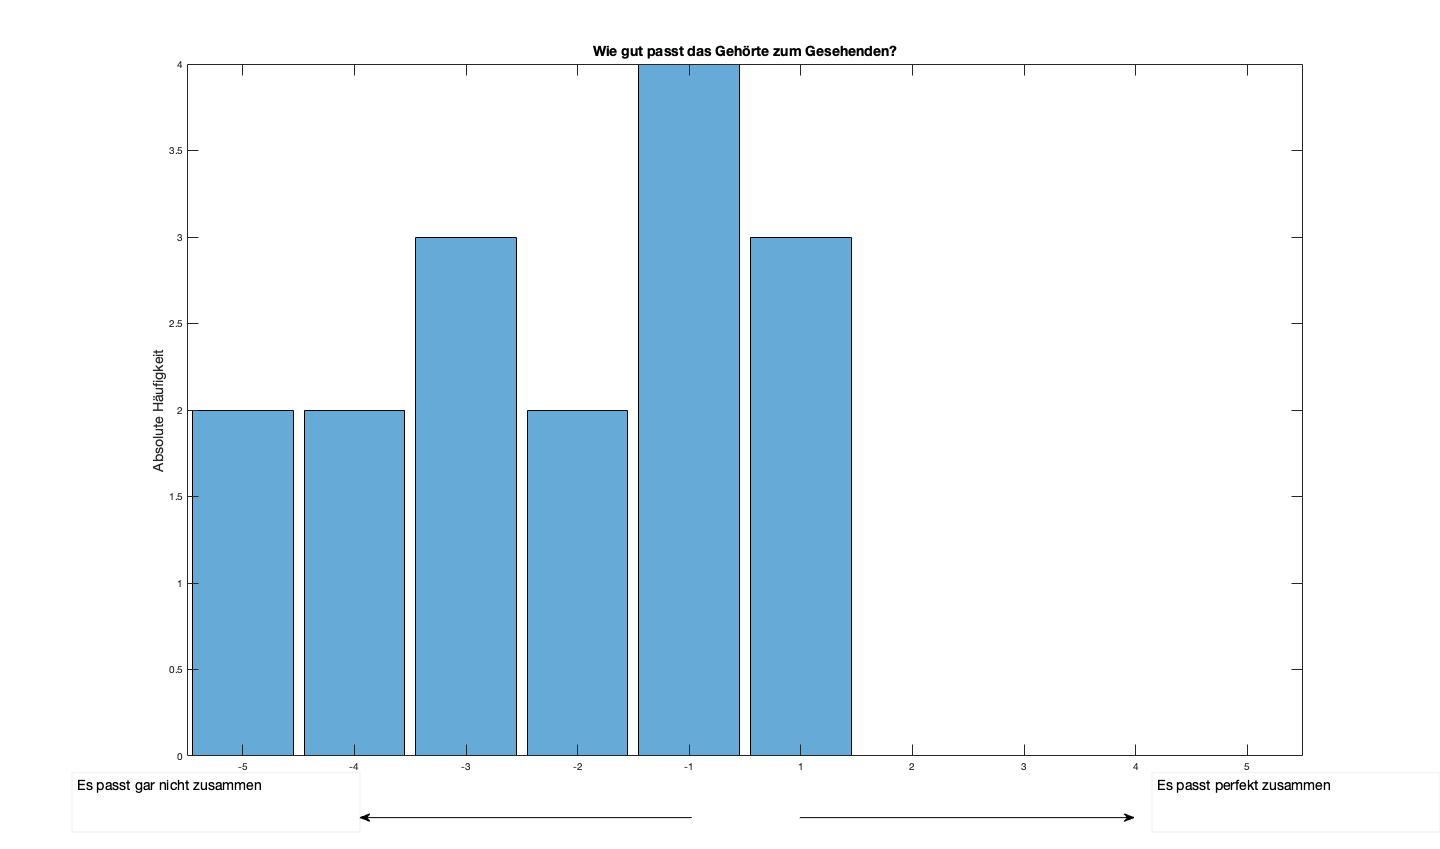
\includegraphics[width = 18cm, height = 10cm]{Szene_5_Frage_1.png}
\caption{Histogramm: Wie gut passen Visuelles und Auditives in Szene 5 zusammen ?}
\label{fig:Szene_5_Frage1}
\end{figure} 

Wie sich in Abbildung \ref{fig:Szene_5_Frage2} erkennen lässt, sind auch bei der Frage, wie echt denn das Geräusch in der letzen Szene wirke, die Probanden fast ausschließlich der Meinung, dass sich das Geräusch sehr realistisch anhört.  Bis auf drei Probanden, die das Geräusch eher als offensichtlich  durch die Kopfhörer wiedergegeben bewertet haben, sind die restlichen Probanden der Meinung, dass sich das Geräusch wirklich so angehört hat als ob die Quelle im Raum wäre.\\ 

Von allen Szenen des Versuches wurde das Geräusch dieser Szene als das realistischste im Raum Hörereignis bewertet. Der Einsatz mehrerer Schallquellen liefert damit also auch mit räumlichem Audio recht plausible Hörereignisse und kann unter anderem dafür genutzt werden größere, virtuelle Objekte auditiv zu unterstützen. \\ 



   \begin{figure}[H]
\centering
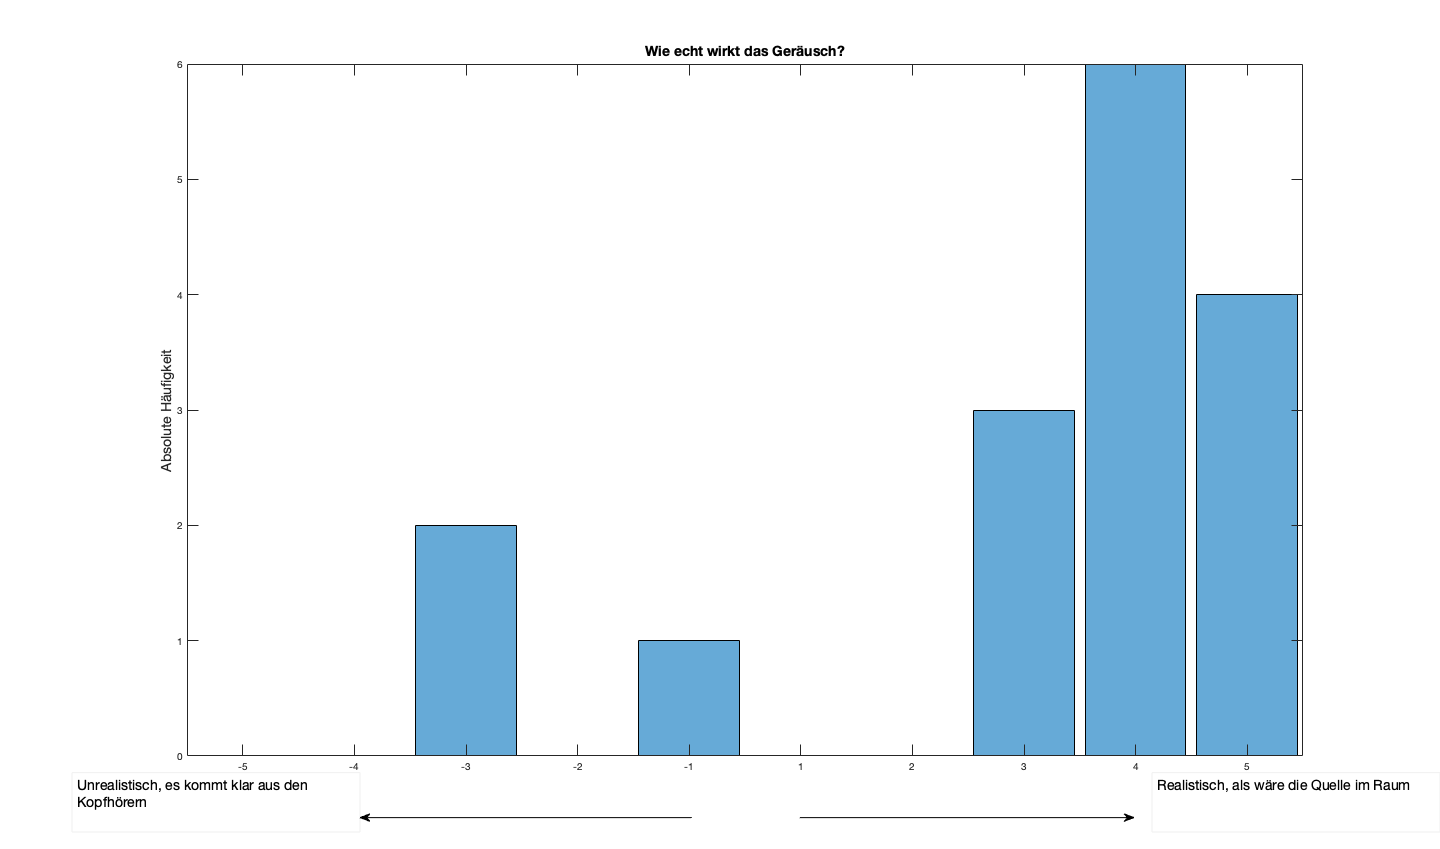
\includegraphics[width = 18cm, height = 10cm]{Szene_5_Frage_2.png}
\caption{Histogramm: Wie echt wirkt das Geräusch im Raum in Szene 5?}
\label{fig:Szene_5_Frage2}
\end{figure} 

Abbildung \ref{fig:Szene_5_Frage3} zeigt, dass auch beim letzten Versuch die Darbietung wieder  als überwiegenden unheimlich bewertet worden ist. Bis auf drei Ausnahmen haben wieder alle Probanden die Darbietung als unheimlich empfunden. Bei keiner Szene vorher wurde hierbei häufiger die maximale Ausprägung des unheimlichen Darbietungsempfindens ausgewählt, wie bei der letzten Szene.\\ 

Auch bei der letzten Szene korrelieren damit die Ergebnisse zum empfunden Realismus des Geräusches mit dem evozierten unheimlichen Darbietungsempfinden. Die These, dass eine realistische Umsetzung von räumlichem Audio Unbehagen auslösen könnte wurde somit durch keine der Darbietungen entschärft und hat weiterhin Bestand. 

   \begin{figure}[H]
\centering
\includegraphics[width = 18cm, height = 10cm]{Szene_5_Frage_3.png}
\caption{Histogramm: Wie angenehm war die Darbietung von Szene 5?}
\label{fig:Szene_5_Frage3}
\end{figure} 

 \section{Ergebnisse kritisch hinterfragen}
 
%Es scheinen für die Lokalisation von virtuelle Schallquellen die ähnliche, psychoakustische Gesetze wie für die Lokalisation von wirklichen Schallquellen zu gelten. Diese These sollte jedoch im Rahmen eines ausführlicheren Hörversuchs unterscuht werden.\\






